\documentclass[11pt,dvipsnames]{report}
\usepackage[utf8]{inputenc}
% \usepackage[T2A]{fontenc}
\usepackage[english, russian]{babel}
% \usepackage{eufrak}
\usepackage{xltxtra}
\usepackage{polyglossia}
\usepackage{mathpazo}
\usepackage{fontspec}

\defaultfontfeatures{Ligatures=TeX,Mapping=tex-text}

\setmainfont[
ExternalLocation={/home/vyacheslav/builds/STIXv2.0.2/OTF/},
BoldFont=STIX2Text-Bold.otf,
ItalicFont=STIX2Text-Italic.otf,
BoldItalicFont=STIX2Text-BoldItalic.otf
]
{STIX2Text-Regular.otf}
\setmathrm{STIX2Math.otf}[
ExternalLocation={/home/vyacheslav/builds/STIXv2.0.2/OTF/}
]

\usepackage{amssymb, amsthm}
\usepackage{amsmath}
\usepackage{mathtools}
\usepackage{needspace}
\usepackage{enumitem}
\usepackage{cancel}
\usepackage{fdsymbol}

% разметка страницы и колонтитул
\usepackage[left=2cm,right=2cm,top=1.5cm,bottom=1cm,bindingoffset=0cm]{geometry}
\usepackage{fancybox,fancyhdr}
\fancyhf{}
\fancyhead[R]{\thepage}
\fancyhead[L]{\rightmark}
% \fancyfoot[RO,LE]{\thesection}
\fancyfoot[C]{\leftmark}
\addtolength{\headheight}{13pt}

\pagestyle{fancy}

% Отступы
\setlength{\parindent}{3ex}
\setlength{\parskip}{3pt}

\usepackage{graphicx}
\usepackage{hyperref}
\usepackage{epstopdf}

\usepackage{import}
\usepackage{xifthen}
\usepackage{pdfpages}
\usepackage{transparent}

\newcommand{\incfig}[1]{%
    \def\svgwidth{\columnwidth}
    \import{./figures/}{#1.pdf_tex}
}

\usepackage{xifthen}
\makeatother
\def\@lecture{}%
\newcommand{\lecture}[3]{
    \ifthenelse{\isempty{#3}}{%
        \def\@lecture{Лекция #1}%
    }{%
        \def\@lecture{Лекция #1: #3}%
    }%
    \subsection*{\@lecture}
    \marginpar{\small\textsf{\mbox{#2}}}
}
\makeatletter

\usepackage{xcolor}
\definecolor{Aquamarine}{cmyk}{50, 0, 17, 100}
\definecolor{ForestGreen}{cmyk}{76, 0, 76, 45}
\definecolor{Pink}{cmyk}{0, 100, 0, 0}
\definecolor{Cyan}{cmyk}{56, 0, 0, 100}
\definecolor{Gray}{gray}{0.3}

\newcommand{\Cclass}{\mathcal{C}}
\newcommand{\Dclass}{\mathcal{D}}
\newcommand{\K}{\mathcal{K}}
\newcommand{\Z}{\mathbb{Z}}
\newcommand{\N}{\mathbb{N}}
\newcommand{\Real}{\mathbb{R}}
\newcommand{\Q}{\mathbb{Q}}
\newcommand{\Cm}{\mathbb{C}}
\newcommand{\Pm}{\mathbb{P}}
\newcommand{\ord}{\operatorname{ord}}
\newcommand{\lcm}{\operatorname{lcm}}
\newcommand{\sign}{\operatorname{sign}}

\renewcommand{\o}{o}
\renewcommand{\O}{\mathcal{O}}
\renewcommand{\le}{\leqslant}
\renewcommand{\ge}{\geqslant}

\def\mybf#1{\textbf{#1}}
\def\selectedFont#1{\textbf{#1}}
% \def\mybf#1{{\usefont{T2A}{cmr}{m}{n}\textbf{#1}}}

% \usefont{T2A}{lmr}{m}{n}
% \usepackage{gentium}
% \usepackage{CormorantGaramond}

\usepackage{mdframed}
\mdfsetup{skipabove=3pt,skipbelow=3pt}
\mdfdefinestyle{defstyle}{%
    linecolor=red,
	linewidth=3pt,rightline=false,topline=false,bottomline=false,%
    frametitlerule=false,%
    frametitlebackgroundcolor=red!0,%
    innertopmargin=4pt,innerbottommargin=4pt,innerleftmargin=7pt
    frametitlebelowskip=1pt,
    frametitleaboveskip=3pt,
}
\mdfdefinestyle{thmstyle}{%
    linecolor=cyan!100,
	linewidth=2pt,topline=false,bottomline=false,%
    frametitlerule=false,%
    frametitlebackgroundcolor=cyan!20,%
    innertopmargin=4pt,innerbottommargin=4pt,
    frametitlebelowskip=1pt,
    frametitleaboveskip=3pt,
}
\theoremstyle{definition}
\mdtheorem[style=defstyle]{defn}{Определение}

\newmdtheoremenv[nobreak=true,backgroundcolor=Aquamarine!10,linewidth=0pt,innertopmargin=0pt,innerbottommargin=7pt]{cor}{Следствие}
\newmdtheoremenv[nobreak=true,backgroundcolor=CarnationPink!20,linewidth=0pt,innertopmargin=0pt,innerbottommargin=7pt]{desc}{Описание}
\newmdtheoremenv[nobreak=true,backgroundcolor=Gray!10,linewidth=0pt,innertopmargin=0pt,innerbottommargin=7pt,font={\small}]{ex}{Пример}
% \mdtheorem[style=thmstyle]{thm}{Теорема}
\newmdtheoremenv[nobreak=false,backgroundcolor=Cyan!10,linewidth=0pt,innertopmargin=0pt,innerbottommargin=7pt]{thm}{Теорема}
\newmdtheoremenv[nobreak=true,backgroundcolor=Pink!10,linewidth=0pt,innertopmargin=0pt,innerbottommargin=7pt]{lm}{Лемма}

\theoremstyle{plain}
\newtheorem*{st}{Утверждение}
\newtheorem*{prop}{Свойства}

\theoremstyle{definition}
\newtheorem*{name}{Обозначение}

\theoremstyle{remark}
\newtheorem*{rem}{Ремарка}
\newtheorem*{com}{Комментарий}
\newtheorem*{note}{Замечание}
\newtheorem*{prac}{Упражнение}
\newtheorem*{probl}{Задача}

\usepackage{fontawesome}
\renewcommand{\proofname}{Доказательство}
\renewenvironment{proof}
{ \small \hspace{\stretch{1}}\\ \faSquareO\quad  }
{ \hspace{\stretch{1}}  \faSquare \normalsize }

%{\fontsize{50}{60}\selectfont \faLinux}

\numberwithin{ex}{section}
\numberwithin{thm}{section}
\numberwithin{equation}{section}

\def\ComplexityFont#1{\textmd{\textbf{\textsf{#1}}}}
\renewcommand{\P}{\ComplexityFont{P}}
\newcommand{\DTIME}{\ComplexityFont{Dtime}}
\newcommand{\DSpace}{\ComplexityFont{DSpace}}
\newcommand{\PSPACE}{\ComplexityFont{PSPACE}}
\newcommand{\NTIME}{\ComplexityFont{Ntime}}
\newcommand{\SAT}{\ComplexityFont{SAT}}
\newcommand{\poly}{\ComplexityFont{poly}}
\newcommand{\FACTOR}{\ComplexityFont{FACTOR}}
\newcommand{\NP}{\ComplexityFont{NP}}
\newcommand{\NPcomp}{\ComplexityFont{NP-complete}}
\newcommand{\BH}{\ComplexityFont{BH}}
\newcommand{\tP}{\widetilde{\P}}
\newcommand{\tNP}{\widetilde{\NP}}
\newcommand{\tBH}{\widetilde{\BH}}
\newcommand{\UNSAT}{{\ComplexityFont{UNSAT}}}
\newcommand{\Class}{{\ComplexityFont{C}}}
\newcommand{\CircuitSat}{{\ComplexityFont{CIRCUIT\_SAT}}}
\newcommand{\tCircuitSat}{\widetilde{{\ComplexityFont{CIRCUIT\_SAT}}}}
\newcommand{\tSAT}{\widetilde{{\ComplexityFont{SAT}}}}
\newcommand{\tThreeSAT}{\widetilde{{\ComplexityFont{3\text{-}SAT}}}}
\newcommand{\ThreeSAT}{{\ComplexityFont{3\text{-}SAT}}}
\newcommand{\kQBF}{{\ComplexityFont{QBF{\tiny k}}}}
\newcommand{\QBFk}{{\ComplexityFont{QBF{\tiny k}}}}
\newcommand{\QBF}{{\ComplexityFont{QBF}}}
\newcommand{\coC}{\ComplexityFont{co-}\mathcal{C}}
\newcommand{\coNP}{\ComplexityFont{co-NP}}
\newcommand{\PH}{\ComplexityFont{PH}}
\newcommand{\EXP}{\ComplexityFont{EXP}}
\newcommand{\Size}{\ComplexityFont{Size}}
\newcommand{\Ppoly}{\ComplexityFont{P}/\ComplexityFont{poly}}

\newcommand{\const}{\textmd{const}}

\usepackage{ upgreek }
\newcommand{\PI}{\Uppi}
\newcommand{\SIGMA}{\Upsigma}
\newcommand{\DELTA}{\Updelta}


\usepackage{minted}

\title{Билеты к экзамену С++ \\ 
    МКН, Современное программирование \\
     семестр I
 }
\author{Тамарин Вячеслав}

\begin{document}
\maketitle
\tableofcontents

% \documentclass[11pt]{book}
\usepackage [utf8] {inputenc}
\usepackage [T2A] {fontenc}
\usepackage[english, russian]{babel}
\usepackage {amsfonts}
\usepackage{eufrak}
\usepackage{amssymb, amsthm}
\usepackage{amsmath}
\usepackage{mathtools}
\usepackage{needspace}
\usepackage{etoolbox}
\usepackage{lipsum}
\usepackage{comment}
\usepackage{cmap}
\usepackage[pdftex]{graphicx}
\usepackage{hyperref}
\usepackage{epstopdf}
\usepackage{enumitem}
\usepackage{mathrsfs}
\usepackage{pb-diagram}

% разметка страницы и колонтитул
\usepackage[left=1.5cm,right=1.5cm,top=2cm,bottom=1.2cm,bindingoffset=0cm]{geometry}
\usepackage{fancybox,fancyhdr}
\fancyhf{}
\fancyhead[R]{\thepage}
\fancyhead[L]{\rightmark}
\addtolength{\headheight}{13pt}
% \fancyfoot[RO,LE]{\thesection}
% \fancyfoot[C]{\leftmark}

\pagestyle{fancy}

\usepackage{import}
\usepackage{xifthen}
\usepackage{pdfpages}
\usepackage{transparent}

\newcommand{\incfig}[1]{%
    \def\svgwidth{\columnwidth}
    \import{./figures/}{#1.pdf_tex}
}

\newcommand{\Z}{\mathbb{Z}}
\newcommand{\N}{\mathbb{N}}
\newcommand{\R}{\mathbb{R}}
\newcommand{\Q}{\mathbb{Q}}
\newcommand{\K}{\mathbb{K}}
\newcommand{\Cm}{\mathbb{C}}
\newcommand{\Pm}{\mathbb{P}}
\newcommand{\ilim}{\int\limits}
\newcommand{\slim}{\sum\limits}
\newcommand{\po}{\diagup}
\newcommand{\op}{\diagdown}
\newcommand{\re}{{\mathop{\text{\rm Re}}\:}}
\newcommand{\GL}{{\mathop{\text{\rm GL}}}}
\newcommand{\ord}{{\mathop{\text{\rm ord}}\:}}
\newcommand{\lcm}{{\mathop{\text{\rm lcm}}\,}}
\newcommand{\sign}{{\mathop{\text{\rm sign}}}}
\newcommand{\del}{{\:\small \raisebox{-2pt}{\vdots}\:}}

\renewcommand{\le}{\leqslant}
\renewcommand{\ge}{\geqslant}
\newcommand{\im}{{\mathop{\text{\rm Im}}}\:}
\renewcommand{\ker}{{\mathop{\text{\rm Ker}}}\:}

\def\mydef{\mathrel{\stackrel{\rm def}=}}
\def\mycheck{\mathrel{\stackrel{\rm ?}=}}

\renewcommand{\thesection}{Вопрос \arabic{section}}
\renewcommand{\thesubsection}{\roman{subsection}}

\renewcommand{\proofname}{Proof}

\usepackage{mdframed}
\mdfsetup{skipabove=0.3em,skipbelow=0.3em}
\theoremstyle{definition}
\newmdtheoremenv[nobreak=true]{defn}{Def}
\theoremstyle{plain}
\newmdtheoremenv[nobreak=true]{thm}{Theorem}

\theoremstyle{plain}
\newtheorem{lm}{Lemma}
\newtheorem{st}{Statement}
\newtheorem*{prop}{Property}
\newtheorem{cor}{Corollary}

\theoremstyle{definition}
\newtheorem*{ex}{Ex}
\newtheorem*{exs}{Exs}
\newtheorem*{name}{Designation}

\theoremstyle{remark}
\newtheorem*{com}{\underline{Comment}}
\newtheorem*{note}{\underline{Note}}


\title{Билеты по алгебре \\ I семестр}
\author{Тамарин Вячеслав}

\begin{document}

\maketitle
% \tableofcontents

\section{Векторное пространство}
\begin{defn}
    Пусть $ (V, +)$ --- абелева группа,  $ F$ --- поле, и задана операция (умножение)  $ V \times F \to  V$. Предположим, что $ \forall  u, v \in V $ и $ \alpha, \beta \in F$ выполнены следующие свойства:
    \begin{enumerate}
	\item  $ v(\alpha \beta) - (v\alpha)\beta$
	\item  $ v(\alpha+\beta) = v\alpha + v\beta$
	\item  $ (v+u)\alpha = v\alpha+v\beta$
	\item  $ v \cdot 1 = v$
    \end{enumerate}
    Тогда $ V$ называется {\sf векторным пространством} над полем  $ F$.
\end{defn}
\begin{prop}
    $ $
    \begin{enumerate}
	\item $ v \cdot 0 = 0 \cdot \alpha  = 0$
	\item $ v \cdot (-1) = -v$
	\item $ v \cdot (-\alpha) = (-v)\alpha = - (v \alpha)$
	\item $v \cdot \sum \alpha_i = \sum v\alpha_i$
	\item $ \sum v_i \cdot \alpha = \sum v_i\alpha$
    \end{enumerate}
\end{prop}
\begin{exs}
    $ $
    \begin{enumerate}
	\item Множество векторов в $\R ^3$
	\item \[
		F^{n} = \left\{
		    \begin{pmatrix}
			a_1 \\ a_2 \\ \vdots \\ a_{n}
		    \end{pmatrix}
		    \middle| a_i \in  F
		\right\}
	    .\]
	    \[
		\begin{pmatrix}
		    a_1 \\ \vdots \\ a_n
		\end{pmatrix}
		\cdot \alpha  =
		\begin{pmatrix}
		    a_1\alpha \\ \vdots \\ a_n \alpha
		\end{pmatrix}
		, \quad
		\begin{pmatrix}
		    a_1 \\ \vdots \\ a_n
		\end{pmatrix}
		+
		\begin{pmatrix}
		    b_1 \\ \vdots \\ b_n
		\end{pmatrix}
		=
		\begin{pmatrix}
		    a_1 + b_1 \\ \vdots \\ a_n + b_n
		\end{pmatrix}
	    .\]
	\item $X$ --- множество, $F^X = \{f \mid f:X \to F\}$ \\
	    $f, g: X \to F$\\
	    $(f+g)(x) = f(x) + g(x)\\ (f \alpha) (x) = f(x)\alpha$
	\item $F[t]$ --- многочлены от одной переменной $t$
    \end{enumerate}
\end{exs}
\section{Подпространство, линейная оболочка}
\begin{defn}
    Подмножество  $ U \subseteq V$ называется {\sf подпространством}, если оно само является векторным пространством относительно тех же операций, которые заданы в $ V$.
\end{defn}
\begin{st}[критерий подпространства]
    Подмножество $ U \subseteq V$ является подпространством тогда и только тогда, когда $ \forall u, v \in U, ~ \alpha \in F: u + v, u \alpha \in U$.
\end{st}
\begin{defn}
    Пусть  $ u_1, \ldots , u_n \in V$, $ \alpha_1, \ldots , \alpha_n \in F$. Сумма
    \[
	\sum _{k = 1}^{n} u_k \alpha_k
    \]
    называется {\sf линейной комбинацией} векторов $ u_1, \ldots , u_n$ с коэффициентами $ \alpha_1, \ldots , \alpha _n$.

    Линейная комбинация называется {\sf тривиальной}, если все ее коэффициенты равны нулю.
\end{defn}
\begin{note}
    Пусть $ S \subseteq V$, и задан набор чисел $ \alpha_s \in F, ~s \in S$. Операция бесконечной суммы будет определена только в случае, когда почти все $ \alpha _s$ равны нулю.
\end{note}
\begin{defn}
    {\sf Линейной оболочкой}  набора $ S$ называется подпространство, порожденное   $ S$, то есть наименьшее подпространство, содержащее  $ S$.
    \begin{name}
	Линейная оболочка  набора $ S$ обозначается   $ \langle S \rangle$.
    \end{name}
\end{defn}
\begin{st}
    $ \langle S \rangle = \left\{ \slim_{k=1}^{n} u_k \alpha_k \middle| u_k\in S, ~ \alpha_k \in F \right\} $
\end{st}
\begin{defn}
    Если $ \langle S \rangle = V$, то $ S$ называется {\sf системой образующих} пространства  $ V$.
\end{defn}
\begin{defn}
    Кортеж векторов $ (u_1, \ldots u_n)$ называется {\sf линейно независимым}, если любая нетривиальная линейная комбинация этих векторов не равна нулю.

    Множество $ S \subseteq V$  называется {\sf линейно независимым}, если любой кортеж  , составленный из конечного числа различных векторов из $ S$, является линейно независимым.
\end{defn}
\begin{defn}
    {\sf Базис} --- линейно независимая система образующих.
\end{defn}
\section{Матрицы}
\subsection{Конечные матрицы}
\begin{defn}
    Двумерный массив  $ m \times n$ элементов поля $ F$ называется {\sf матрицей} размера  $ m \times  n$ над $ F$.
    \begin{name}
	Множество таких матриц  обозначается $ M_{m \times n}(F)$. Если $ m = n$, пишут  $ M_n(f)$.
	Элемент матрицы $ A$ в позиции  $ (i, j)$ записывается  $ a_{ij}$.
    \end{name}
\end{defn}
\begin{prop}
    $ $
    \begin{itemize}
	\item Для двух матриц одинакового размера определена операция поэлементной суммы: $ (A + B)_{ij} = a_{ij } + b_{ij}$.
	\item Также определено умножение матрицы на число: $ (A\alpha)_{ij } = a_{ij} \alpha$.
	\item Произведением матрицы $ A \in M_{m \times n}(F)$ на матрицу $ B \in M_{n \times k}$  называется матрица $ C = AB \in M_{m \times  k}(F)$ элементы которой вычисляются по формуле
	    \[
		c_{ij} = \sum _{l=1}^{n}a_{il}b_{lj}
	    .\]
    \end{itemize}
\end{prop}
\begin{thm}\label{prop_multi_matr}
    Множество $ M_{m \times n}(F)$ с операциями сложения и умножения на число является векторным пространством над полем $ F$.
\end{thm}
\begin{proof}
    Произведение матриц ассоциативно, дистрибутивно и  перестановочно  с умножением на число:
    \[
	\begin{cases}
	    (AB)C = A(BC)\\
	    A(B+C) = AB + BC\\
	    (B+C)A=BA + CA\\
	    (AB)\alpha = A(B\alpha) = (A\alpha)B
	\end{cases}
    .\]
    Все кроме первого свойства очевидны. Проверим ассоциативность:
    \[
	\begin{aligned}
	    \left( (AB) C \right)_{il} &= \sum _{k \in K} (AB)_{ik} c_{kl} = \sum_{k \in K}\left( \sum_{j \in J} a_{ij}b_{jk} \right)  c_{kl}  = \\
				       &= \sum_{k \in K} \left( \sum _{j \in J} a_{ij} b_{jk} c_{kl}\right) = \\
				       &= \sum _{j \in J} \left( \sum _{k \in K} a_{ij} b_{jk} c_{kl} \right) = \\
				       &= \sum _{j \in J} a_{ij} \left( \sum _{k \in K}b_{jk} c_{kl} \right) = \sum _{j \in J} a_{ij} (BC) _{jl} = \left( A(BC) \right)_{il}
	\end{aligned}
    .\]
    \begin{defn}
	Квадратная матрица  $ E$ с 1 на главной диагонали и остальными нулями называется {\sf единичной}.
    \end{defn}
    \begin{prop}
	Умножение данной матрицы на единичную справа и слева не ее не изменяет.
    \end{prop}
    Матрица $ E_n$ является нейтральным элементом в $ M_n(F)$.
\end{proof}
\subsubsection{Обобщение конечных матриц}
Пусть даны множества $ X_{ij}, Y_{jh}$, коммутативные моноиды $ (Z_{ih}, +)$, где $ i = 1, \ldots m, ~ j = 1, \ldots n, ~ h= 1, \ldots k$, и функции <<умножения>> $ X_{ij} \times Y_{jh} \to  Z_{ih}, ~ (x, y) \mapsto xy$.  Обозначим через $ X, Y, Z$ наборы множеств  $ X_{ij}, Y_{jh}, Z_{ih}$, соответственно, через $ M(X)$ --- множество матриц  $ A$ с элементами  $ a_{ij} \in X_{ij}$, и аналогично $ M(Y), M(Z)$. Тогда можно определить произведение матриц $ A \in M(X)$ и $ B \in M(Y)$ как матрицу $ C = AB \in M(Z)$, где $ c_{ih} = \sum\limits_{j = 1}^{n}a_{ij}b_{jh}$.

Если все $ X_{ij}, Y_{jh}$ будут коммутативными моноидами, а функция умножения дистрибутивной, умножение матриц тоже будет дистрибутивным и ассоциативным.
\subsection{Произвольные матрицы}
Пусть  $ I, J$ --- произвольные множества (возможно бесконечные), элементами которых мы будем индексировать строки и столбцы матриц. Пусть  $ \forall i \in I \wedge j \in J$ задано множество $ X_{ij}$, и обозначим набор всех таких множеств через $ X$.
Тогда {\sf матрицей размера $ I \times J$ над $ X$}  называется функция  $ A: I \times J \to \bigcup X_{ij} ~ (i, j) \mapsto a_{ij}$, такая что $ a_{ij} \in X_{ij}$.
\begin{name}
    Множество матриц размера $ I \times J$ над $ X$ обозначается  $ M_{I \times J}(X)$.
    Если $ I = \{1\}$, то матрица размера $ I \times J$ будут назваться столбцами длины $ J$, а если  $ J = \{1\}$, то столбцами высоты $ I$. Множества строк обозначим данной длины $ ^J\!X$, множество столбцов --- $ X^{J}$.
\end{name}
Будем считать, что все $ X_{ij}$ --- абелевы группы в аддитивной записи. Тогда сумма двух матриц одного размера определяется поэлементно: $ (A+B)_{ij} = a_{ij}+b_{ij}$.
Если все $ X_{ij}$ --- векторные пространства над полем $ F$, также можно определить умножение на число:  $ (A\alpha)_{ij} = a_{ij}\alpha$.
\subsubsection{Умножение матриц}
Пусть все операции умножения  $ X_{ij}\times Y_{jh} \to Z_{ih}$ дистрибутивны (для $ a \cdot 0 = 0$), и в каждом столбце матрицы $ Y$ почти все элементы равны 0.
\begin{name}
    Обозначим $ M_{J\times H}^{c.f.}(Y) \subset M_{J\times H}(Y)$, состоящее из всех матриц $ B$, у которых для любого фиксированного  $ h \in H$ почти все элементы $ b_{jh}$ равны 0.
\end{name}
\begin{defn}
    Пусть $ \forall i \in I, j \in J, h \in H$ заданы операции умножения $ X_{ij} \times Y_{jh} \to  Z_{ih}$, причем $ \forall  x, x' \in X_{ij}$ и $ \forall y, y' \in Y_{jh}$ выполнены равенства
    \[
	(x+x')y = xy + x'y \wedge x(y + y') = xy + xy'
    .\]
    Произведение матриц $ A \in M_{i \times J}(X)$  и $ B \in <_{J\times H}^{c.f.}(Y)$ как матрицу $ AB \in M_{I \times H}(Z)$ с элементами
    \[
	(AB)_{ih} = \sum_{j \in J}a_{ij}b_{jh}
    .\]
    При этом суммы определены, так как почти все слагаемые равны нулю.
\end{defn}
\begin{note}
    Аналогично определяется умножение матриц $ A \in M_{I \times J}^{r.f.}(X)$ и $ B \in M_{J \times H}(Y)$.
\end{note}
\begin{lm}
    Обычные свойства умножения матриц \ref{prop_multi_matr} выполнены, если определены все входящие в формулы операции.

    Если $ \forall i, j, h \in I$ заданы дистрибутивные операции умножения $ X_{ij} \times X_{jh} \to  X_{ih}$, то множество $ M_{I \times I}^{c.f.}(X)$ является кольцом с единицей.
\end{lm}
\begin{name}
    Если $ X_{ij}$ одно и то же поле $ F$ для всех  $ i, j$, будем писать  $ M_{i\times J}(F)$ вместо $ M_{I\times J} (X)$. Если $ I = J$, то будем писать  $ M_{I}(F)$ вместо $ M_{I \times I}(F)$. Если $ I = \{1, \ldots m\}, J= \{1, \ldots n\}$, то можем писать $ M_{m \times n}(F)$.
\end{name}
\subsubsection{Другие характеристики матриц}
\begin{defn}
    Множество обратимых элементов кольца $ M_n(F)$ называется  {\sf полной линейной группой} степени  $ n$ над  $ F$ и обозначается  $ \GL_{n}(F)$.
\end{defn}
\begin{name}
    Для множества $ M_{I \times \{1\}}^{c.f.}(F)$ введем специальное обозначение $ F^{I}_{fin}$ и будем называть его {\sf множеством финитных столбцов} высоты $ I$ над  $ F$. Другим словами, $ F_{fin}^{I}$ --- множество финитных (у которых почти все значения равны 0) функций из $ I$ в  $ F$.
    Аналогично, $ ^J\!F_{fin}= M_{\{1\}\times J}^{r.f.}(F)$.
\end{name}
\begin{defn}
    Пусть $ A \in M_{I \times J}(F)$. Матрица $ A^{T} \in M_{J \times I}(F)$ с элементами $ (A^{T})_{ij} = a_{ji}$ называется {\sf транспонированной} к $ A$.
\end{defn}
\begin{st}
    $ (AB)^{T} = B^{T}A^{T}$
\end{st}
\begin{note}
    Для обозначения столбца часто используется строка $ (a_1, \ldots a_n)^{T}$.
\end{note}
\section{Эквивалентные определения базиса}
\begin{thm}[Эквивалентные определения базиса]
    Следующие условия на подмножество $ v$ векторного пространства  $ V$ эквивалентны:
    \begin{enumerate}[label={\rm (\arabic*)},noitemsep]
	\item $ v$ --- линейно независимая система образующих
	\item $ v$ --- максимальная линейно независимая система
	\item $ v$ --- минимальная система образующих
	\item  любой элемент  $ x \in V$ представляется в виде линейной комбинации набора $ v$, причем единственным образом
    \end{enumerate}
\end{thm}
\begin{proof}
    $ $
    \begin{description}
	\item $ \boxed{1 \Longrightarrow 2}$ Пусть $ v$ ---  не максимальная линейно независимая система. Мы знаем, что $ v$ --- система образующих. Тогда любой элемент  $ a \in V$ представляется в виде линейной комбинации $ v$, а значит любой набор, содержащий  $ v$, принадлежит линейной оболочке  $ \langle v \rangle$, следовательно, набор линейно зависимый.
	\item $ \boxed{2 \Longrightarrow 1}$
	    Так как $ v$ максимальная линейно независимая система, любой элемент  $ a \in V$ выражается через элементы $ v$. Следовательно,  $ v$ --- система образующих.
	\item $ \boxed{1 \Longrightarrow 3}$ Пусть из $ v$ можно убрать некоторые элементы так, что полученный набор $ u$ будет минимальной системой образующих. Тогда любой элемент набора  $ v \smallsetminus u$ представим в виде линейной комбинации $ u$. Следовательно,  $ v$ линейно зависим.
	\item $ \boxed{3 \Longrightarrow 1}$ Если $ v$ линейно зависим, то во всех линейных комбинациях набора  $ v$ можно заменить один элемент на линейную комбинацию других. А тогда  $ v$ не минимален.
	\item  $ \boxed{1 \Longrightarrow 4}$ Так как $ v$ --- система образующих  $ \langle v \rangle = V$. Теперь докажем, что представление единственно. Пусть $ x = va = \sum_{y \in v} y a_y, \quad a \in F^{v}_{fin}$.
	    Предположим, что $ \exists b \in F_{fin}^{v}: x = vb$. Тогда  $ 0 = va - vb \Longrightarrow 0 = v(a-b)$. Так как $ v$ линейно независим, можем сократить:  $ 0 = a-b$, значит представление единственно.
	\item $ \boxed{4 \Longrightarrow 1}$ Так как любой элемент представим в виде линейной комбинации набора $ v$,  $ \langle v \rangle = V$. Так как представление единственно, $ v$ линейно независим.
    \end{description}
\end{proof}
\section{Существование базиса}
\begin{thm}[О существовании базиса]
    Пусть $ X, Y \subseteq V$, причем набор $ X$ линейно независим, а  $ Y$ --- система образующих. Тогда существует базис  $ Z$, содержащий  $ X$ и содержащийся в  $ Y$.
\end{thm}
\begin{proof}
    Пусть $ \mathscr{A}$ --- набор всех линейно независимых подмножеств $ Y$, содержащих $ X$.  Этот набор не пуст, так как содержит  $ X$.
    Пусть  $ \mathscr L$ --- линейно упорядоченный поднабор в  $ \mathscr A$. Обозначим через $ S$ объединение всех множеств из  $ \mathscr L$.
    Так как $    \forall C \in \mathscr L
    $ лежит между  $ X$ и  $ Y$, $ S$ обладает этим свойством.
    Рассмотрим конечное подмножество $ \{v_1, \ldots v_n\} \subseteq S$. По определению объединения множеств $ \forall i = 1, \ldots n ~ \exists B_i \in \mathscr L$, содержащее $ v_i$. Так как  $ \mathscr L$ --- лум, среди множеств $ B_1, \ldots B_n$ найдется наибольшее $ B_k$. Тогда $ v_1, \ldots v_n \in B_k$. Так как $ B_k$ линейно независимо, то и  $ \{v_1, \ldots v_n\}$ линейно независимо. Следовательно, $ S$ линейно независимо, значит  $ S \in \mathscr A$.
    По лемме Цорна получаем, что $ \mathscr A$ содержит максимальных элемент. Пусть это  $ Z$ --- максимальное из линейно независимых подмножеств $ Y$, содержащих  $ X$.

    Пусть $ y \in Y \setminus Z$. Так как $ Z$ линейно независимо,  $ Z \cup \{y\}$ линейно зависимо, то есть $ \exists a \in F^{Z}_{fin}, ~a_y \in F: ya_y + Za = 0$, где $ a_y \ne 0$. Следовательно, $ y \in \langle Z \rangle$. Тогда $ Y \subseteq \langle Z \rangle$. С другой стороны, $ V = \langle Y \rangle$ --- наименьшее подпространство,  содержащее $ Y$. Значит  $ V \subseteq \langle V \rangle $, то есть $ Z$ --- система образующих, следовательно, и базис.
\end{proof}
\section{Лемма о замене}
\begin{thm}[лемма о замене]\label{lm_zam}
    Пусть $ u = \{u_1, \ldots u_n\}$ --- линейно  независимый набор из  $ n$ векторов, $ v$ --- система образующих пространства  $ V$.
    Тогда:
    \begin{enumerate}[noitemsep]
	\item $ \exists v_1, \ldots v_n \in v: v \smallsetminus \{v_1, \ldots v_n\} \cup u = w$ --- система образующих.
	\item Причем, если  $ u$ --- базис, то $ w$ --- базис.
    \end{enumerate}
\end{thm}
\begin{proof}
    Индукция по $ n$.
    \begin{description}
	\item База: $ n = 0$.  Утверждение для нуля верно.
	\item Переход:  $ n-1 \to  n$. По предположению индукции $ \exists v_1, \ldots v_{n_i} \in v$ такие, что $ w' = v \smallsetminus \{v_1, \ldots v_{n-1}\} \cup \{u_1, \ldots u_{n-1}\}$ является системой образующих. Причем, если $ v$ был линейно независимым, то  $ w'$ --- базис.

	    $ u_n$ выражается через линейную комбинацию набора  $ w'$:  \[
		u_n =	      \sum_{i=1}^{n-1} u_i \alpha_i + \sum _{j=1}^{m} w_{j}\beta_j, \qquad \alpha_i, \beta_j \in F, w_j \in v \smallsetminus \{v_1, \ldots v_{n-1}\}
	    .\]
	    Заметим, что кто-то из $ \beta_j \ne 0$ (иначе $ u$ линейно зависим).
	    Не умоляя общности, считаем, что $ \beta_m \ne 0$.  Пусть $ v_n = w_m$. Тогда  $ v_n$ выражается через линейную комбинацию набора  $ w = w' \smallsetminus \{v_n\} \cup \{u_n\}$. Следовательно, $ w' \subseteq \langle w \rangle$, значит $ w$ --- система образующих.

	    Пусть набор  $ v$ (а тогда и  $ w'$) линейно независим. Рассмотрим  $ w'' = w' \smallsetminus \{v_n\}$ и линейную комбинацию $ w'' a + u_n \alpha $ набора  $ w$, где  $ a \in F_{fin}^{w''}$.
	    \[
		0 = w'' a + u_n \alpha = w''a + \sum _{i=1}^{n-1} u_i \alpha_i \alpha + \sum _{j= 1}^{m} w_i \beta_j \alpha = w'' b + v_n \beta_m \alpha, \qquad b \in F_{fin}^{w''}
	    .\]
	    Если $ \alpha \ne 0$, то $ w''b + v_n \beta_m \alpha$ является нетривиальной линейной комбинацией набора  $ w'' \cup \{v_n\} = w''$, равной нулю. Значит,  $ \alpha =0$, тогда $ w''a = 0$. Так как  $ w'' \subseteq w'$, $ w''$ линейно независим, следовательно,  $ a = 0$.

	    Получаем, что  $ w$  линейно независим.
    \end{description}
\end{proof}
\section{Количество элементов в базисе}
\begin{thm}[количество элементов в базисе]
    Любые два базиса пространства $ V$ равномощны.
\end{thm}
\begin{proof}
    Пусть $ v, u = \{u_1, \ldots u_n\}$ ---  базисы пространства $ V$. Не умоляя общности, считаем, что мощность множества  $ v > n$. Перенумеруем элементы базиса  $ u$ так, что $ u_1, \ldots u_k \not\in v$ и $ u_{k+1}, \ldots  v_n \in v$.

    Тогда по лемме о замене \ref{lm_zam} существует подмножество $ \{v_1, \ldots v_k\} \subseteq v: w = v \smallsetminus \{v_1, \ldots v_k\} \cup \{u_1, \ldots u_k\}$ --- базис. $ u \subseteq w$ и $ |v|  = |w|$. Так как базис --- максимальная линейно независимая система, то один базис не может строго содержаться в другом. Следовательно, $ w = u$, откуда  $ |v|  = n$.
\end{proof}
\begin{defn}
    {\sf Размерность пространства} --- мощность любого базиса этого пространства.

    Пространство называется {\sf конечномерным}, если в нем существует конечный базис.
\end{defn}
\section{Линейные отображения и их матрицы. Матрица композиции линейных отображений}
\subsection{Линейные отображения}
\begin{defn}
    Пусть $ V$ и  $ U$ --- векторные пространства,  $ L$ --- функция  $ V \to  U$. $ L$ называется {\sf линейным отображением}, если
    $
    \forall x, y \in V, ~ \alpha \in F:
    $
    \[
	\begin{aligned}
	    & L(x+y) = L(x) + L(y) \\
	    & L(x\alpha) = L(x) \alpha
	\end{aligned}
    \]
    Биективное линейное отображение называется {\sf изоморфизмом}.
    Линейное отображение из пространства в само себя называется {\sf линейным оператором}.
    Отображение из пространства в основное поле часто называется {\sf функционалом}.
\end{defn}
\begin{prop}
    Пусть вектор $ v = (v_1, \ldots v_n)$ и  отображение $ L: V \to U$. \[
	L(v) = (L(v_1), \ldots L(v_n)) \in ^n\!\!U
    .\]
    Тогда
    \[
	L(va) = L(v)a, \text{ где } a \in F^{n}
    .\]
    \begin{note}
	В случае бесконечного $ v$ можем переписать аналогично, обозначив  $ L(v) \in ^n\!\!U: L(v)_x = L(x) \quad \forall x \in v$:
	\[
	    L(va) = L(v)a, \text{ где } a \in F^{v}
	.\]
    \end{note}
\end{prop}
\begin{name}
    Пусть $ v$ --- базис  $ V$. Тогда  $ \forall x \in V ~ \exists ! a \in F_{fin}^{v}: x = va$.
    Тогда $ a = x_v$ --- столбец координат  $ x$ в базисе  $ v$.
\end{name}
\begin{lm}
    Пусть $ V$ --- векторное пространство над полем  $ F$, а  $ v$ --- базис  $ V$. Отображение  $ \varphi _v: V \to  F^{v}$, заданное равенством $ \varphi _v(x) = x_{v}$, является изоморфизмом векторных пространств.
\end{lm}
\begin{proof}
    Рассмотрим $ x, y \in V$.
    \[
	\begin{cases}
	    v x_v = x \\
	    v y_v = y
	\end{cases}
	\Longrightarrow v(x_v + y_v) = x+y = v(x+y)_v \Longrightarrow \varphi_v (x+y) = \varphi_v (x) + \varphi_v (y)
    .\]
    \[
	v(x\alpha)_v = x\alpha = v(x_v \alpha) \Longrightarrow  \varphi_v (x\alpha) = \varphi_v(x)\alpha
    .\]
    Построим обратное отображение:
    $ \theta_v: F^{v} \to  V, ~ \theta_v(a) = va$.
    Следовательно, $ \varphi _v$ --- биективное линейное отображение.
\end{proof}
\begin{cor}[классификация векторных пространств]
    Любое векторное пространство изоморфно пространству $ F^{I}$ для некоторого множества $ I$, мощность которого равна размерности пространства.

    Два пространства изоморфны между собой  тогда и только тогда, когда их размерности равны.
\end{cor}
\subsection{Матрицы линейных отображений}
\begin{st}\label{st_m_o}
    Пусть $ L : U \to  V$ --- линейное отображение, $ u = (u_1, \ldots u_n) $ --- базис $ U$,  $ v=(v_1, \ldots v_m)$ --- базис $ V$.
    \[
	\exists ! A \in M_{m \times n}(F): \forall x \in U ~ L(x)_v = Ax_u
    .\]
    Столбцы матрицы $ A$ вычисляются по формуле $ a_{*k}=L(u_k)_v$.
\end{st}
\begin{proof}
    По определению столбца координат $ x = ux_u$.   \[
	\varphi _v \circ L(x) = \varphi _v \circ L(ux_v)
    .\]
    Тогда $ L_(x)_v = \varphi _v\bigl(L(x)\bigr) = \varphi _v\bigl(L(u)\bigr)x_u$.
    Пусть $ A = \varphi _v\bigl(L(u)\bigr) = \bigl( L(u_1)_v, \ldots L(u_n)_v \bigr)$.

    Докажем единственность. Предположим, что $ Ax = Bx$ для любого столбца  $ x$. Тогда  $ A = B$.
\end{proof}
\begin{defn}
    Матрица $ A$ из прошлого утверждения \ref{st_m_o} называется {\sf матрицей отображения} $ L$ в базисах  $ u, v$ и обозначается через  $ L_u^{v}$.

    Если $ U = V$,  $ u = v$, говорят о матрице оператора  $ L$ в базисе  $ u$ и обозначают ее через  $ L_u$.
    \[
	L(x)_v = L_u^{v}x_v \text{ или } L(x)_u = L_ux_u \text{ в случае } U=V \wedge u=v
    .\]
\end{defn}
\begin{thm}
    Матрица композиции линейных операторов является произведением матриц этих операторов.

    Если $ U, V, W$ --- конечномерные линейный пространства с базисами  $ u, v, w$, соответственно,  $ L: U \to V, ~ M: V \to W$ --- линейные отображения,  то $ (M \circ L)_u^{w}= M_v^{w}L_u^{v}$.

    Если $ U = V = W$ и  $ u = v = w$, то  $ (M \circ L)_u=M_uL_u$.
\end{thm}
\section{Матрица перехода от одного базиса с другому. Замена координат и изменение матрицы оператора при замене базиса}
\subsection{Матрица перехода}
\begin{thm}
    Пусть $ v$ --- базис  $ n$-мерного пространства  $ V$ над полем  $ F$. Набор  $ u = (u_1, \ldots u_n)$ является базисом тогда и только тогда, когда существует $ A \in \GL _n (F)$ такая, что $ u = vA$.
    \begin{defn}
	Если  $ u, v$ --- базисы, то  $ A$ называется {\sf матрицей перехода}  от $ v$ к  $ u$ и обозначается через  $ C_{v \to  u}$
    \end{defn}
    При этом:
    \begin{enumerate}[noitemsep,label={\rm (\arabic*)}]
	\item Столбец матрицы $ C_{v \to u}$ с номером  $ k$ равен столбцу координат вектора $ u_k$ в базисе  $ v$.  $ (C_{v \to  u})_k = (u_k)_v$
	\item $ C^{-1}_{v \to  u} = C_{u \to  v}$
	\item Если матрица двусторонне обратима, то она квадратная.
    \end{enumerate}
\end{thm}
\begin{proof}
    $ $
    \begin{description}
	\item \boxed{  \Longrightarrow }  Положим $ \forall k \in [1, n]: a_{*k} = (u_k)_v$. Тогда $ va_{*k} = u_k \Longrightarrow u = vA$
	\item \boxed{  \Longrightarrow } Если $ u = vA$,  $ \langle u  \rangle = \langle vA \rangle = V$. При этом $ u$ минимален, так как иначе и  $ v$ не минимален, значит  $ u$ --- базис.
    \end{description}
    \begin{enumerate}[noitemsep]
	\item По построению.
	\item  $
	    \begin{cases}
		u = v C_{v \to  u}\\
		v = u C_{u \to  v}
	    \end{cases} \Longrightarrow uE = uC_{u \to  v} C_{v \to  u} \Longrightarrow E = C_{u \to  v} C_{v \to  u}
	    $
	\item Пусть  $ B \in M_{n \times m}(F)$ двусторонне обратима.  $ B B_1 = E_{n\times n} \wedge B_2 B = E_{m\times m}$. Тогда  $ B_2 = B_2 E_{n} = B_2(B B_1)=(B_2 B) B_1 = E_m B_1 = B_1$. Значит $ B_1 = B_2$. $ B_1B = C_{u \to  v}C_{v \to  u} = B_1B \Longrightarrow B \text{ --- квадратная}$.
    \end{enumerate}
\end{proof}
\begin{note}
    Если пространство $ V$ бесконечномерно,  почти все элементы каждого столбца должны быть равны нулю.
\end{note}
\begin{note}
    Если $ V = F^{n}$, $ e$ --- стандартный базис, то  $ C_{e \to  u}$ --- матрица, составленная из столбцов базиса $ u$.
\end{note}
\subsection{Преобразование координат при замене базиса}
\begin{thm}
    Пусть $ u, v$ --- базисы пространства  $ V$.
    \[
	\forall x \in V: x_v = C_{v \to  u}x_u
    .\]
\end{thm}
\begin{proof}
    Запишем определение столбца координат $ x = ux_u  = vx_v$.
    Про базисы мы знаем, что  $ v = u C_{u \to  v}$. Тогда
    \[
	ux_u = u C_{u \to  v} x_v \Longrightarrow x_u = C_{u \to  v} x_v
    .\]
\end{proof}
\subsection{Преобразование матрицы оператора при замене базиса}
\begin{note}
    Матрица перехода $ C_{u \to  v}$ совпадает с матрицей тождественного отображения $ 1_{V}$ в базисах $ u$ и  $ v$.
\end{note}
\begin{lm}
    Пусть $ u  = (u_1, \ldots u_n)$ --- базис пространства $ U$,  $ v = (v_1, \ldots v_n) \in ^n\!\!V$ --- набор векторов пространства $ V$. Тогда существует единственное линейное отоббражение
    \[
	L: U \to V: L(u) = v
    .\]
    При этом
    \begin{description}[noitemsep]
	\item $ L$ инъективно  тогда и только тогда, когда $ u$ линейно независим
	\item $ L$ сюрьективно  тогда и только тогда, когда $ u$ --- система образующих
	\item $ L$ --- изоморфизм  тогда и только тогда, когда  $ u $ --- базис
    \end{description}
\end{lm}
\begin{proof}
    $ \forall x \in U: x = ux_u$. Тогда $ \forall L: L(x) = L(u)x_u$. Зададим $ L$ так:  $ L(x) = v x_u$. Оно линейно и единственно.
\end{proof}
\begin{note}
    Пусть $ u, v$ --- базисы пространства  $ V$. Тогда  матрица отображения  $ L$ из леммы в базисе $ u$ совпадает с  матрицей перехода  $ C_{u \to  v}$.
\end{note}
\begin{st}
    Пусть $ u, u'$ --- базисы пространства  $ U$,  $ v, v'$ --- базисы пространства  $ U$,  $ v, v'$ --- базисы пространства  $ V$,  $ L: V \to  U$ --- линейное отображение. Тогда
    \[
	L_{u'}^{v'} = C_{v' \to  v}L_{u}^{v}C_{u \to  u'}
    .\]
\end{st}
\begin{proof}
    \begin{align*}
	& L(x)_v = L_u^{v}x_u\\
	& C_{v' \to  v} L(x)_v = L(x)_{v'} = L_{u'}^{v'}x_{u'}=L_{u'}^{v'}C_{u' \to  u} x_u\\
	& L(x)_{v} = C_{v \to  v'}L_{u'}^{v'}C_{u' \to u}x_u\\
	& L_{u}^{v} = C_{v \to v'}L_{u'}^{v'}C_{u' \to u}
    \end{align*}
\end{proof}
\begin{note}
    Если $ U = V$ и  $ u = v, ~ u' = v'$,
    \[
	L_{u'} = C_{u' \to  u} L_u C_{u \to  u'}
    .\]
\end{note}
\section{Внешняя и внутренняя пряма сумма пространств, естественный изоморфизм между ними}
\begin{name}
    $ U, V$ --- подпространства векторного пространства  $ W$ над полем  $ F$.
\end{name}
\begin{defn}
    Сумма $ U + V$ --- совокупность  $ \{x + y \mid x \in U, y \in V\}$.
    \begin{note}
	$ U + V \subseteq W \wedge  U \cap V \subseteq W$.
    \end{note}
\end{defn}
\begin{defn}
    Пространство $ W$ называется {\sf внутренней прямой суммой} подпространств $ U$ и  $ V$, если   $$ \forall z \in W ~ \exists ! x \in U, y \in V: z = x+y.$$ То есть $ W = U + V \wedge V \cap U = \{0\}$.
\end{defn}
\begin{defn}
    $ U, V$ --- векторные пространства.  Их  {\sf внешней прямой суммой} называется их декартово произведение с покомпонентыми операциями.
\end{defn}
\begin{name}
    Обе прямые суммы обозначаются $ U \oplus V$.
\end{name}
\begin{note}
    Пространства $ U, V$ естественно вкладываются в из внешнюю прямую сумму:  $ \forall x \in U: x \mapsto (x, 0) \wedge  \forall y \in V: y \mapsto (0, y)$. Если отождествить $ U$ и  $ V$ с их образами, то внешняя сумма превращается в прямую сумму подпространств.
\end{note}
\begin{st}
    $ U, C \le W$, $ U \oplus V$ --- их внешняя прямая сумма. Зададим  $ \varphi : U \oplus V \to W$ так $ \varphi (x, y) = x + y$. $ \varphi $ --- изоморфизм тогда и только тогда, когда $ W $ является внутренней суммой подпространств  $ U$ и  $ V$.
\end{st}
Если $ W = U \oplus V$, то объединение базисов  $ U$ и  $ V$ --- базис  $ W$. Поэтому  $ \dim(U \oplus V) = \dim(U) + \dim(V)$.
\begin{st}
    $ \forall U \le W ~ \exists V \le W: W = U \oplus V$.
\end{st}
\begin{proof}
    Выберем базис  $ u$ подпространства  $ U$ и дополним его до базиса пространства  $ W$: $ u \cup v$. Тогда подойдет $ V = \langle v \rangle$.
\end{proof}
\begin{thm}
    Для пространств $ U_1, \ldots U_n \le V$ следующие условия эквивалентны:
    \begin{enumerate}[noitemsep,label={\rm (\arabic*)}]
	\item  $ U_1 \oplus \ldots U_n \to V, ~ (x_1, \ldots x_n) \mapsto x_1 + \ldots x_n$ --- изоморфизм
	\item $ \forall x \in V ~ \exists ! \bigl(x_1 \in U_1, \ldots x_n \in U_n\bigr): x =x_1 + \ldots x_n$
	\item $ V = U_1+ \ldots U_n$ и $ U_i \cap \left( \sum_{j\ne i}U_{j} \right)=\{0\} \qquad i \in [1, n]$
	\item Объединение базисов подпространств $ U_1, \ldots U_n$ --- базис $ V$.
    \end{enumerate}
\end{thm}
\section{Ядро и образ линейного отображения. Слои линейного отображения}
\begin{defn}
    Пусть $ L: U \to V$ --- линейное отображение. Тогда
    \begin{description}[noitemsep]
	\item {\sf Ядро отображения $ L$ --- }  $ \ker L = L^{-1}(0) \coloneqq \{x \in U \mid L(x) = 0\}$
	\item {\sf Образ отображения $ L$ --- } $ \im L = \{L(x) \mid x \in U\}$
    \end{description}
\end{defn}
\begin{st}
    Пусть $ L: U \to  V$ --- линейное отображение.
    \[
	\ker L \le U \wedge  \im  L \le U
    .\]
\end{st}
\begin{defn}
    $ L : U \to  V$ --- линейное отображение.
    {\sf Слой} отображения над точкой $ y \in V$ --- множество $ \{x \in X\mid L(x) = y\} = L^{-1} (y)$
\end{defn}
\begin{st}
    Все слои отображения $ L$ являются сдвигами ядра.  $ L(x) = y, ~ x \in U$:
    \[
	L^{-1}(y) = x + \ker L
    .\]
\end{st}
\section{Теорема о размерности ядра и образа. Теорема о размерности прямой суммы}
\begin{thm}[о размерности ядра и образа]
    $L: U \to V$ --- линейное отображение. Тогда
    \[
	\dim U = \dim \ker L + \dim \im L
    .\]
\end{thm}
\begin{proof}
    $u = (u_1, \ldots u_k)  \text{ --- базис } \ker L,	~
    v = (v_1, \ldots v_m)$.
    Дополним базис ядра до базиса $U$:
    $u \cup v $ --- базис $U$.
    Докажем, что $L(v) = \left(L(v_1), L(v_2), \ldots L(v_m)\right)$ --- базис образа.

    $$ \forall  x \in \im L~  \exists y \in U: L(y) = x.$$
    Разложим $y = ua + vb , \qquad a \in F^k, ~b \in F^m $ \\
    Тогда
    \[
	x = L(y) = {{L(u)}}\cdot a + L(v)\cdot  b
    .\]
    Так как $ u \in \ker: L( u)= \left( L(u_1), \ldots L(u_k) \right) = (0, \ldots 0)$.
    Следовательно, $L(v)$ --- система образующих. Проверим, что $ L(v)$ линейно независим.
    Пусть
    \[
	L(v)\cdot  c = 0, \quad c \in F^m
    .\]
    \[
	L(v) c = L(vc) = 0 \Rightarrow vc \in \ker L \Rightarrow vc = ud \mbox{ для некоторого } d \in F^k
    .\]
    Тогда $vc - ud = 0$, но $v$ и $u$ --- два базисных вектора. Следовательно, $c=d=0$ и $L(v)$ --- линейно независимый.
\end{proof}
\begin{thm}[формула Грассмана о размерности суммы и пересечения]
    Пусть $U, V \le W$.
    \[
	\dim U\cap V + \dim U+V = \dim U + \dim V
    .\]
\end{thm}
\begin{proof}
    Зададим линейное отображение $ L: U \oplus V \to  W: L(u, v) = u+v$.
    Тогда $\im L = U+V$.
    $$
    (u, v) \in \ker L \Longleftrightarrow  u + v = 0 \Longleftrightarrow  u = -v \in  U\cap V
    .$$
    $$
    \ker L = \{(u, -u) \mid u \in U \cap V\} \cong U\cap V
    .$$
    По теореме о размерности ядра и образа
    $$
    \dim U + \dim V = \dim (U \oplus V) = \dim \ker L + \dim \im L = \dim U \cap V + \dim U+V
    .$$
\end{proof}
\section{Факторпространство и его универсальное свойство}
\begin{name}
    $ V$ --- векторное пространство,  $ U \le V$.
\end{name}
\begin{defn}
    $ x + U$ --- аффинное подпространство или смежный класс  $ V$ по  $ U$.

    $ y \sim _{U} x \Longleftrightarrow y - x \in U$ --- эквивалентность.
\end{defn}
\begin{defn}
    Множество смежных классов $ V$ по  $ U$ с операциями
    \begin{align*}
	(x + U) + (y + U) &= (x+ y) + U  \\
	(x + u) \alpha &= x\alpha + U
    \end{align*}
    называется {\sf факторпространством} $ V$  по  $ U$ и обозначается  $ V / U$.
\end{defn}
\begin{proof}[Проверка корректности определения]
    Докажем, что определение операций не зависит от выбора представителей классов.
    \begin{itemize}
	\item Сложение \[
		x' + U = x + U \Longrightarrow x' + 0 \in x + U \Longrightarrow x' \in x + U
	    .\]
	    \[
		y' + U = y + U \Longrightarrow y' + 0 \in y + U \Longrightarrow y' \in y + U
	    .\]
	    Тогда $ \exists z \in U: x' = x + z$ и $ \exists t \in U: y' = y + t$.
	    \begin{align*}
		(x' + U) + (y' + U) & \coloneqq (x' + y') + U = \\
				    &= (x+y) + \underbrace{(z+t)}_{ \in U} + U \subseteq \\
				    &\subseteq (x+y) + U
	    \end{align*}
	    Аналогично доказываем включение в обратную сторону.
	\item  Умножение
	    \begin{align*}
		(x' + U) \alpha & \coloneqq x'\alpha + U = \\
				& = (x + z)\alpha + U = x\alpha + \underbrace{z\alpha}_{ \in U} + U \subseteq \\
				& \subseteq x\alpha + U
	    \end{align*}
	    Аналогично доказываем включение в обратную сторону.
    \end{itemize}
\end{proof}
\begin{name}
    $ \pi_U: V \to  V / U$ ---  естественная проекция: $ \pi_U(x) = x + U$.
    \begin{note}
	$ \pi_U$ линейно и сюрьективно  $ \ker \pi_U = U$.

	По теореме о размерности ядра и образа
	$\dim V / U = \dim V - \dim U $.:
    \end{note}
\end{name}
\begin{st}\label{st_l_ker}
    Пусть $ U \subseteq V$. Для любого линейного отображения $ L: V \to W$, $ U \subseteq \ker L$, существует единственное отображение $ \tilde L: V / U \to  W: L = L \circ \pi_U$.
    При этом сюрьективность  $ \tilde L$  равносильна сюрьективности $ L$, а инъективность  $ \tilde L$ --- тому, что  $ \ker L = U$.
    То есть такая диаграмма коммутативна:
    $$
    \begin{diagram}
	\node{V} \arrow[1]{e,t}{L}
	\arrow{s,l}{\pi_U}
	\node[1]{W} \\
	\node{V / U} \arrow[1]{ne,b}{\tilde L}
    \end{diagram}
    $$
\end{st}
\begin{proof}
    Пусть $ \tilde L(x + U) = L(x)$. Эта формула задает линейное отображение и равносильна $ L = \tilde \pi_U$. Следовательно, $ \tilde L$ существует и единственно.

    $ \pi_U$  инъективно, следовательно, $ L$ сюрьективно  $ \Longleftrightarrow $ $ \tilde L$ сюрьективно.

    Отображение  $ \tilde L$ инъективно  $ \Longleftrightarrow \ker \tilde L = \{0_{V / U} + U\}$.
    \[
	x + U \in \ker \tilde L \Longleftrightarrow \tilde L(x + U) = 0 \Longleftrightarrow L(x) = 0 \Longleftrightarrow x \in \ker L
    .\]
\end{proof}
\begin{thm}[о гомоморфизме]
    $L : V \to W$ --- линейное отображение.
    \[
	V / \ker L \cong \im L
    .\]
\end{thm}
\begin{proof}
    Возьмем $U = \ker L$ и заменим $W$ на $\im L$. Далее применим утверждение \ref{st_l_ker}.
\end{proof}
\section{Ранг набора элементов векторного пространства, ранг оператора, строчной и столбцовый ранг матрицы}
\begin{defn}
    $ $
    \begin{description}[noitemsep]
	\item {\sf Рангом набора векторов} называется размерность линейной оболочки этого набора.
	\item {\sf Рангом линейного оператора} называется размерность образа этого оператора.
	\item {\sf Столбцовым (строчным) рангом матрицы} называется ранг набора ее столбцов (строк).
    \end{description}
\end{defn}
\begin{note}
    Из любой системы образующих можно выбрать базис, следовательно, ранг набора векторов --- наибольшее количество линейно независимых векторов из этого набора. Так как образы базисных векторов порождают образ оператора, то ранг оператора равен рангу набора базисных векторов, а он равен столбцовому рангу матрицы оператора (вне зависимости от выбора базиса).
\end{note}
\begin{thm}
    Пусть $ A \in M_{m \times n}(F)$.
    \begin{enumerate}[noitemsep,label={\rm (\arabic*)}]
	\item Набор столбцов матрицы $ A$ линейно независим  тогда и только тогда, когда ее столбцовый ранг равен $ n$.
	\item Набор столбцов матрицы  $ A$ порождает  $ F^{m}$ тогда и только тогда, когда ее столбцовый ранг равен $ m$.
	\item Набор столбцов матрицы $ A$ является базисом в  $ F^{m}$ тогда и только тогда, когда ее столбцовый ранг $ m = n$. В этом случае  $ A$ обратима.
	\item Если все строки матрицы $ A$ линейно независимы, и все столбцы линейно независимы, то $ m = n$, а  $ A$ обратима.
    \end{enumerate}
\end{thm}
\begin{proof}
    Пункты $ (1)$ и  $ (2)$ очевидны. Из них следует, что столбцовый ранг равен $ m = n$  тогда и только тогда, когда набор столбцов --- базис в $ F^{m}$. В этом случае $ A$ --- матрица перехода от стандартного базиса к базису из столбцов матрицы  $ A$, а значит  $ A$ обратима.

    Количество линейно независимых столбцов и строк не может быть больше размерности, следовательно,  $ n \le m \wedge n \ge m \Longrightarrow n = m$.
\end{proof}
\begin{lm}
    Умножение матрицы на обратимую (слева или справа) не меняет ее столбцовый и строчной ранги.
\end{lm}
\begin{proof}
    Умножение матрицы оператора слева на обратимую матрицу соответствует замене базиса в его области значений, а справа --- в области определения. Так как столбцовый ранг оператора не зависит от выбора базиса, то столбцовый ранг не меняется при умножении.

    Строчный ранг равен столбцовому рангу транспонированной к ней, а транспонированная к обратимой --- обратима.
\end{proof}
\section{PDQ-разложение. Равенство строчного и столбцового рангов матрицы}
\begin{thm}[PDQ-разложение]
    Пусть $ U, V$ --- конечномерные пространства. Для любого линейного отображения $ L: U \to  V$ существуют базисы пространств $ U$ и  $ V$, в которых матрица  отображения $ L$ имеет вид  $
    \begin{pmatrix}
	E & 0 \\ 0 & 0
    \end{pmatrix}$.

    Любая матрица $ A \in M_{m\times n}(F)$ представляется в виде $ A = PDQ$, где  $ P \in \GL_M(F), ~ Q \in \GL_n(F)$, а $ D$ записывается в блочном виде  $ D =
    \begin{pmatrix}
	E & 0 \\ 0 & 0
    \end{pmatrix}$. При этом размер единичной матрицы равен строчному и столбцовому рангу $ A$.
\end{thm}
\begin{proof}
    $ $
    \begin{description}
	\item $\boxed{\text{Первое утверждение}}$ Выберем базис $ (f_1, \ldots f_k)$ ядра оператора $ L$ и дополним его до базиса  $ u = (g_1, \ldots g_l, f_1, \ldots f_k)$ пространства $ U$.
	    Тогда векторы $ L(g_1), \ldots L(g_l)$ линейно независимы и их можно дополнить до базиса $ v$ пространства  $ V$. Получаем нужную матрицу отображения  $ L$ в базисах  $ u, v$.
	\item  $ \boxed{\text{Второе утверждение}}$ Пусть $ L: F^{n} \to  F^{m}$ --- оператор умножения на матрицу $ A$. Выберем базис  $ u$ пространства  $ F^{n}$ и $ v$ --- пространства $ F^{m}$ так, чтобы $ L_v^{u} = D$.
	    Тогда
	    \[
		A = A_{e}^{e} = C_{e \to  u}L_{v}^{u}C_{v \to  e} = PQD
	    ,\]
	    где $ e$ --- стандартный базис пространства столбцов.

	    Так как ранги при умножении  обратимую матрицу не меняются, столбцовый и строчной ранги равны рангу единичной матрицы.
    \end{description}
\end{proof}
\begin{lm}
    Квадратная матрица обратима тогда и только тогда, когда е ранг равен ее размеру.
\end{lm}
\begin{thm}[Кронокера-Капелли]
    Система $ Ax = b$ совместима  тогда и только тогда, когда ранг матрицы $ A$ равен рангу расширенной матрицы  $ \left( A b \right) $.
\end{thm}
\section{Разложение Брюа}
\begin{defn}
    Матрица $ A$ называется {\sf верхней (нижней) треугольной}, если $ a_{ij} = 0 \quad \forall i  > j ~(i < j)$.

    Треугольная матрица с 1 на диагонали называется {\sf унитреугольной}.
    \begin{name}
	$ $
	\begin{description}[noitemsep]
	    \item $ B = B_n(F)$ --- множество верхних треугольных матриц.
	    \item $ B^{-} = B_{n}^{-}(F)$ --- множество нижних треугольных матриц.
	    \item $ U = U_{n}(F)$ --- множество верхних унитреугольных матриц.
	    \item $ U^{-} = U^{-}_{n}(F)$ --- множество  нижних унитреугольных матриц.
	    \item $ W = W_n$ --- множество матриц перестановок, то есть матрицы, отличающиеся от единичной перестановкой столбцов.
	\end{description}
    \end{name}
\end{defn}
\begin{lm}
    Множества  $ W, B, B^{-}, U, U^{-}$ являются подгруппами в $ \GL_{n}(F)$.
\end{lm}
\begin{thm}[разложение Брюа]
    $ \GL_n(F) = BWB$
\end{thm}
\begin{proof}
    Докажем, что $ \forall a \in \GL_n(F) ~ \exists b, c \in D, ~ w \in W: a = bwc$.
    \begin{description}
	\item По индукции  по $ n$ докажем, что, домножая $ a$  слева и справа на верхнетреугольные матрицы, можно получить матрицу перестановку.

	    Пусть $ i$ ---  наибольший индекс, для которого  $ a_{i 1} \ne 0$. Запишем $ a$ в виде
	    \[
		a =
		\begin{pmatrix}
		    x & * \\
		    a_{i 1} & z \\
		    0 & *
		\end{pmatrix}
		, \quad \text{где } x =
		\begin{pmatrix}
		    a_{1 1} \\
		    \vdots \\
		    a_{i - 1 1}
		\end{pmatrix}, ~ \text{ a } z - (a _{i 2}, \ldots a_i n)
	    .\]
	    Домножая $ a$ слева на верхнетреугольныую матрицу, получим матрицу, у которой первый столбец совпадает с  $ i$-м столбцом единичной матрицы.
	    После этого, домножая справа на подходящую верхнереугольныю матрицу можем сделать $ i$-ю строку равной первой строке единичной матрицы:
	    \[
		\begin{pmatrix}
		    E& -\frac{x}{a_{i 1}}& 0 \\
		    0 & \frac{1}{a_{ i 1}} & 0 \\
		    0 & 0 & E
		\end{pmatrix}
		\begin{pmatrix}
		    x & * \\
		    a_{i 1} & z \\
		    0 & *
		\end{pmatrix}
		\begin{pmatrix}
		    1 & -\frac{z}{a_{i 1}}\\
		    0 & E
		\end{pmatrix}
		=
		\begin{pmatrix}
		    0 & f\\
		    1 & 0 \\
		    0 & g
		\end{pmatrix}
		\quad \text{ для некоторых матриц } f, g
	    .\]
	    Заметим, что так как строки полученной матрицы линейно независимы, то и строки матрицы $
	    \begin{pmatrix}
		f \\ g
	    \end{pmatrix}$
	    тоже линейно независимы. Поэтому последняя матрица обратима и к ней можно применить индукционное предположение. Следовательно, существуют матрицы $ u, v \in B_{n-1}(F): u
	    \begin{pmatrix}
		f \\ g
	    \end{pmatrix}
	    v \in W_{n-1}$.
	    Пусть
	    \[
		u =
		\begin{pmatrix}
		    u^{(1)} & u^{(2)} \\
		    0 & u^{(3)}
		\end{pmatrix}
	    , ~\text{ где } u^{(1)} \in B_{i-1}(F), ~ u^{(3) }\in B_{n-i}(F).\]
	    Тогда
	    \[
		\begin{pmatrix}
		    u^{(1)} & u^{(2)} \\
		    0 &u^{(3)}
		\end{pmatrix}
		\begin{pmatrix}
		    f \\ g
		\end{pmatrix}
		\cdot  v
	    \]
	    является матрицей-перестановкой, следовательно,
	    \[
		\begin{pmatrix}
		    u^{(1)} & 0 & u^{(2)} \\
		    0 & 1 & 0 \\
		    0 & 0 & u^{(3)}
		\end{pmatrix}
		\begin{pmatrix}
		    0 & f \\
		    1 & 0 \\
		    0 & g
		\end{pmatrix}
		\begin{pmatrix}
		    1 & 0 \\
		    0 & v
		\end{pmatrix}
	    \]
	    --- тоже матрица-перестановка.
	\item Так как обратная к верхнетреугольной --- верхнетругольная, получаем нужное утверждение.
    \end{description}
\end{proof}
\begin{defn}
    Множество $ B w B$ при фиксированном $ w$ называется {\sf клеткой Брюа}.
\end{defn}
\begin{st}
    Две различные клетки Брюа не пересекаются.
\end{st}
\section{Разложение Гаусса}
\begin{defn}
    {\sf Главная подматрица} матрица $ A$ порядка  $ k$ --- подматрица, стоящая на пересечении первых $ k$ строк и первых $ k$ столбцов.
\end{defn}
\begin{lm}
    Умножение матрицы на нижнюю унитреугольную слева и на верхнюю унитреугольную справа не меняет обратимости главных подматриц.
\end{lm}
\begin{proof}
    $a^{(k)}$ --- главная подматрица $k \times k$ в $a$.
    Умножим на нижнюю унитреугольную матрицу слева:
    \[
	\left (
	    \begin{array}{cc}
		b&0\\
		c&1
	    \end{array}
	\right )
	\left (
	    \begin{array}{cc}
		a^{(k)}&* \\
		*& *
	    \end{array}
	\right )=
	\left (
	    \begin{array}{cc}
		ba^{(k)}&*\\
		*&*
	    \end{array}
	\right )
    .\]
    $\mbox{Где } b \in  U^-(F)$.
    Обратимость $a^{(k)} $ равносильна обратимости $ba^{(k)}$, так как $b$ обратима.
\end{proof}
\begin{lm}
    Все главные подматрицы обратимы тогда и только тогда, когда матрица раскладывается в произведение обратимых унитреугольных верхнетреугольной и нижнетреугольной.
\end{lm}
\begin{proof}
    Доказываем следствие влево.
    Индукция по $n$.
    \begin{description}
	\item База: $n=1$ --- очевидно\\
	\item Переход: \\
	    \[
		a^{(n)} =
		\left (
		    \begin{array}{cc}
			a^{(n-1)} & * \\
			* & a_{nn}
		    \end{array}
		\right )
	    .\]
	    \[
		\left (
		    \begin{array}{cc}
			1&0\\-xa^{(n-1)}&1
		    \end{array}
		\right )
		\left (
		    \begin{array}{cc}
			a^{(n-1)} & *\\
			x&a_{nn}
		    \end{array}
		\right )=
		\left (
		    \begin{array}{cc}
			a^{(n-1)}&*\\0&*
		    \end{array}
		\right )
	    .\]
	    Дальше применим предположение индукции к $a^{(n-1)}$. Она раскладывается в произведение верхне- и нижнетреугольной.
    \end{description}
    В обратную сторону следует из прошлой леммы.
    Действительно, у обратимой верхнетреугольной матрицы все главные подматрицы обратимы, а умножение слева на обратимые	нижнетреугольные не меняет их обратимость.
\end{proof}
\begin{lm}
    $\forall a \in  \GL_n(F) ~ \exists w \in  W : $ все подматрицы в $wa$ обратимы.
\end{lm}
\begin{proof}
    Индукция по $k$.
    Докажем, что существует перестановка $a \in  \GL_n(F)$ такая, что главные подматрицы размера не более $k \times k$ обратимы.
    \begin{description}
	\item База: $k=1$ \[
		a_{*1} = 0 \Rightarrow \exists i: a_{ij} \ne 0
	    .\] Меняем $i$-ю строку с первой.
	\item Переход: $ k \to  k+1$
	    Все столбцы обратимой матрицы линейно независимы, следовательно, ранг матрицы, составленной из первых $ k$ столбцов, равен  $ k$
	    Тогда существует $ k$ линейно независимых строк  этой матрицы.
	    Переставим эти строки на первые $ k$ мест.
	    \[
		a =
		\left (
		    \begin{array}{cc}
			a^{(k)}& *\\
			* & *
		    \end{array}
		\right )
	    .\]
	    У полученной матрицы $ a^{(k)}$ главная подматрица порядка $ k$ обратима.
	    По индукционному предположению все меньшие главные подматрицы в $a^{(k)}$ обратимы.
    \end{description}
\end{proof}
\begin{thm}[Разложение Гаусса]
    $ \GL_{n}(F) = WB^{-}B$
\end{thm}
\begin{proof}
    Рассмотрим $ a \in \GL_{n}(F)$. Построим перестановку $ w$, чтобы все главные подматрицы были обратимы. Дальше домножим справа и слева на унитреугольные матрицы так, чтобы получить верхнетругольную матрицу:
    $wa \in  B^- B$. Домножая на $B, B^-$, получим, что хотели.
\end{proof}

\section{Определение группы, подгруппы, прямое произведение групп}
\begin{defn}
    Множество $X$ с операцией $*$ , удовлетворяющее
    \begin{enumerate}
	\item $\forall x,y,z \: \in X: x*(y*z) = (x*y)*z$  (ассоциативность);
	\item $\exists e \in X \; \forall a \in X: e*a = a*e = a$ (нейтральный элемент);
	\item $\forall a \in X \; \exists a' \in X: a*a' = a' * a = e $ (обратный элемент),
    \end{enumerate}
    называется {\sf группой}.
\end{defn}
\begin{defn}
    Непустое подмножество $H \subset G$ называется {\sf подгруппой} $ G$, если $H$ --- группа относительно операции, заданной в $G$.
    \begin{name}
	Обозначается: $H \le G$
    \end{name}
\end{defn}
\begin{lm}
    $H \subset B$.
    $H$ --- подгруппа тогда и только тогда, когда $ \forall h, g \in H: gh, g^{-1} \in  H$.
\end{lm}
\begin{prop}
    Любая группа имеет две тривиальные подгруппы: сама группа и множество, состоящее из одного нейтрального элемента.
\end{prop}
\begin{defn}
    Пусть  $ G_1, G_2$ --- группы с операциями  $ *_1$ и $ *_2$ соответственно. {\sf Прямое произведение}  $ G = G_1 \times G_2$ --- декартово произведение  $ G_1$ и $ G_2$ c операцией $ *$:
    \[
	(g_1, g_2) * (g_1', g_2') = (g_1 *_1 g_1', g_2*_2 g_2'), \quad g_1, g_1' \in G_1, ~ g_2, g_2' \in G_2
    .\]

    Аналогично определяется произведение любого семейства групп.
\end{defn}
\section{Подгруппа, порожденная множеством. Классификация циклических подгрупп}
\begin{defn}
    Пусть $ X$ --- подмножество группы  $ G$.  {\sf Подгруппой, порожденной множеством}  $ X$, называется наименьшая группа по включению, содержащая  $ X$.
    \begin{name}
	Подгруппа, порожденная  $ X$, обозначается $ \langle X \rangle$.
    \end{name}
\end{defn}
\begin{defn}
    Группа, порожденная одним элементом, называется {\sf циклической}.
\end{defn}
\begin{lm}
    $ \langle X \rangle = \{x_1 \ldots x_k \mid k \in \Z_+, ~ x_i \in X \cap X^{-1}\}$.
\end{lm}
\begin{st}
    Любая циклическая группа изоморфна $\Z$ или $\Z_n$.
\end{st}
\begin{proof}
    $G = \{g^m \mid m \in \Z\}$. Разберем два случая:
    \begin{enumerate}
	\item $g^m \ne 1 \quad  \forall m \in  \Z \Longrightarrow \nexists a, b \in \Z: g^{a} = g^{b}$.
	    Тогда отображение
	    \[
		\varphi : \Z \to  G, \quad \varphi (m) = g^m
	    \text{ --- изоморфизм}.\]
	    \[
		\varphi (m+k) = g^{m+k} = g^m g^k = \varphi (m) \varphi (k)
	    .\]
	\item Пусть $n$ --- наименьшее натуральное число, такое, что $g^n = 1$.
	    Заметим, что любое целое $ l$ можно с остатком разделить на  $ n: l = ns + r, ~ 0 \le r < n$.
	    Тогда \[
		g^{l} = g^{ns}g^{r} = g^{r}
	    .\]
	    Следовательно, $ \langle g \rangle = \{1, g, g^2, \ldots g^{n-1}\}$.
	    Тогда отображение
	    \[
		\varphi : G \to \Z_n, \quad k \to  g^{k} \text{ --- изоморфизм}
	    .\]
    \end{enumerate}
\end{proof}
\section{Смежные классы по подгруппе. Теорема Лагранжа}
\begin{defn}
    Пусть $ H \le G$. Множества $ gH$ и  $ Hg$ называются {\sf левым и правым смежными классами по подгруппе} $ H$ соответственно.
    \begin{name}$ $
	\begin{description}[noitemsep]
	    \item
		$G \diagup H = \{gH \mid g \in G\} $ --- множество левых смежных классов.
	    \item
		$H \diagdown G = \{Hg \mid g \in G\} $ --- множество правых смежных классов.
	\end{description}
    \end{name}
\end{defn}
\begin{defn}
    Отношение сравнимости по модулю $ H$:
    \[
	a \equiv b \mod H  \Longleftrightarrow a \in bH
    .\]
\end{defn}
\begin{lm}
    Сравнимость по модулю $ H$ --- отношение эквивалентности. Два смежных класса либо не пересекаются, либо совпадают.
\end{lm}
\begin{proof}
    $ $
    \begin{description}[noitemsep]
	\item Рефлексивность: $ a = ae \in a H$
	\item Симметричность: $ a \in B \Longrightarrow \exists h \in H: a= bh \Longrightarrow  b=a h^{-1} \in  aH$
	\item Транзитивность: $ a \in bH, b \in cH \Longrightarrow a = bh, b = ch' \Longrightarrow a = chh' \in c H$
    \end{description}
    Второе утверждение вытекает из того, что классы сравнимости --- левые смежные классы по подгруппе.
\end{proof}
\begin{cor}
    $$G =\bigsqcup\limits_{g \in X} g H, \text{ где } X \text{ --- множество представителей левых смежных классов по $H$}$$
\end{cor}
\begin{lm}
    \[
	|g_1H| = |g_2H|, \quad \forall g_1, g_2 \in  G,~ H \le G
    .\]
\end{lm}
\begin{proof}
    Такое отображение будет изоморфизмом:
    \[
	\left (
	    \begin{array}{c}
		g_1H \to g_2H \\
		x \mapsto g_2 g_1^{-1} x
	    \end{array}
	\right )
    .\]
    Обратное: $y \mapsto g_1 g_2^{-1} y$
\end{proof}
\begin{thm}[Лагранж]
    $G$ --- конечная группа. Тогда $|G| = |H|\cdot  |G:H|$, где $|G:H|$ --- количество левых смежных классов $G$ по $H$.
    $|G:H|$ --- индекс $H$ в $G$.
\end{thm}
\begin{proof}
    Из прошлой леммы и следствия
\end{proof}
\begin{lm}
    Множества $ G \po H$ и $ H \op G$ равномощны.
\end{lm}
\begin{proof}
    Зададим биекцию $ \varphi : G \po H \to  H \op G, \quad aH \mapsto (aH)^{-1} = Ha^{-1}$.
\end{proof}
\section{Порядок элемента группы.}
\begin{defn}
    {\sf Порядок} $g \in  G$ --- наименьшее натуральное число, такое что $g^n = 1$.

    Второе определение:
    $\ord(g) = | \langle g \rangle|$.
\end{defn}
\begin{thm}
    Пусть $ G$ --- группа,  $ g \in G$. Тогда $|G| \del \ord (g)$
\end{thm}
\begin{proof}
    Применим теорему Лагранжа для подгруппы порожденной $ g: |G| \del |\langle g \rangle|, ~ \ord(g) = |\langle g \rangle|$
\end{proof}
\begin{thm}
    Пусть $ \varphi : G \to H $ --- гомоморфизм. $ g \in G, ~ \ord(g) = n$. Тогда $\ord(g) \del \ord(f(g)) $.
\end{thm}
\begin{proof}
    \[
	1_H =	f(1_G) = f(g^{n}) = f(g)^{n} \Longrightarrow n \del \ord(f(g))
    .\]
\end{proof}
\begin{st}
    Пусть $ G$ --- абелева группа,  $ a, b \in G$. Тогда $\lcm (\ord (a), \ord(b)) \del  \ord(ab) $.
\end{st}
\begin{proof}
    Обозначим $\lcm (\ord (a), \ord(b)) = n, ~ \ord(ab) = m$
    \[
	(ab)^{n} = a^{n}b^{n} = 1 \Longrightarrow  n \del m
    .\]
\end{proof}
\begin{thm}\label{th_ords}
    Пусть $ G$ --- абелева группа,  $ a, b \in G, ~ \gcd(\ord (a), \ord(b)) = 1 $. Тогда $ \ord (ab) = \ord(a) \ord(b)$.
\end{thm}
\begin{proof}
    Рассмотрим $ \langle a \rangle \cap \langle b \rangle  = H$. Это подгруппа $ \langle a \rangle$ и $ \langle b \rangle$. По теореме Лагранжа $ \ord (a) \del |H|$ и $ \ord (b) \del |H|$.
    Так как порядки $ a$ и  $ b$ взаимно просты, $ \langle a \rangle \cap \langle  b \rangle = \{e\}$. Тогда
    \[
	a^{s} = b^{t} \Longleftrightarrow a^{s} = b^{t} = e
    .\]
    Это равносильно тому, что
    \[
	s \del \ord(a), ~ t \del \ord(b)
    .\]
    Если $ (ab)^{n} = e$, то $ a^{n} = b^{-n}$, значит $ n \del\ord(a) \wedge n \del \ord(b)$. Порядки взаимно просты, следовательно $ n \del \ord(a)\ord(b)$. С другой стороны, по прошлому утверждению  $ \ord(a)\ord(b) \del \ord(ab)$. Следовательно,  \[
	\ord(a)\ord(b) = \ord(ab)
    .\]
\end{proof}
\section{Экспонента группы, критерий цикличности группы}
\begin{defn}
    {\sf Экспонентой} или {\sf показателем} группы $ G$ называется натуральное число  $ d: g^{d} = e \quad \forall g \in G$. Если такого $ g$ не существует, то говорят, что экспонента группы равна бесконечности.
\end{defn}
\begin{thm}[свойства экспоненты группы]
    $ $
    \begin{enumerate}[noitemsep,label={\rm (\arabic*)}]
	\item Экспонента группы равна НОКу всех порядков ее элементов.
	\item Если группа конечна, то ее экспонента делит ее порядок.
	\item Экспонента прямого произведения групп $ G_1\times \ldots G_l$ равна НОКу экспонент этих групп.
	\item \label{p_peg}Если $ G$ --- абелева группа конечной экспоненты, то существует элемент, порядок которого равен ее экспоненте.
	\item Конечная абелева группа является циклической  тогда и только тогда, когда ее экспонента равна ее порядку.
    \end{enumerate}
\end{thm}
\begin{proof}
    Докажем пункт \ref{p_peg}. Пусть $ d = p_1^{k_1} \cdot  \ldots p_l^{k_l}$ --- экспонента группы $ G$, где  $ p_1, \ldots p_l \in \Pm$. Тогда $ \exists  g_1, \ldots g_l \in G$, порядки которых делятся на $ p_1^{k_1}, \ldots p_l^{k_l}$ соответственно.

    Если $ \ord(g) = mn$, то  $ \ord (g^{m}) = n$. Возведем $ g_1, \ldots g_l$ в нужные степени и считаем, что $ \ord(g_i) = p_{i}^{k_i} \quad \forall  i \in [1, l]$.

    Воспользуемся теоремой \ref{th_ords}, и по индукции докажем, что $ \ord(g_1\cdot  \ldots g_l) = \ord(g_1) \cdot  \ldots \ord(g_l) = d$.
\end{proof}
\section{Нормальные подгруппы. Гомоморфизмы групп. Свойства ядра и образа.}
\subsection{Нормальные подгруппы}
\begin{defn}
    Пусть $H \le G$.
    $H$ называется {\sf нормальной подгруппой}, если $gH = Hg \quad g \in  G$.
    \begin{name}
	Обозначается: $H \trianglelefteq G$.
    \end{name}
\end{defn}
\begin{note}
    $g^{-1} H g = H \quad \forall g \in  G \Longleftrightarrow  g^{-1} H g \subseteq H \quad \forall g \in  G \Longleftrightarrow H \trianglelefteq G$
\end{note}
\subsection{Гомоморфизмы групп}
\begin{defn}
    Пусть $ (G, *), ~ (H, \#)$ --- группы. Функция $ f: G \to  H$ называется {\sf гомоморфизмом}, если  $ f(a \cdot b) = f(a)\#f(b) \quad \forall a, b \in G$.

    Образ гомоморфизма $ \im f = \{f(g) \mid g \in G\}$.

    Ядро гомоморфизма $ \ker f = \{g \in G\mid f(g)=e_H \}$.
\end{defn}
\begin{defn}
    $ $
    \begin{description}[noitemsep]
	\item {\sf Мономорфизм} --- инъективный гомоморфизм.
	\item {\sf Эпиморфизм} --- сюрьективный гомоморфизм.
	\item {\sf Изоморфизм} --- биективный гомоморфизм.
    \end{description}
\end{defn}
\begin{lm}
    Если $ f: G \to H$ --- гомоморфизм групп, $ f(e_G) = e_H$ и  $ \forall x \in G: f(x^{-1}) - f(x) ^{-1}$
\end{lm}
\begin{lm}
    Пусть $ f: G \to  H$ --- гомоморфизм групп, $ g \in G, ~ h= g(g)$. Тогда $ f^{-1}(h) - g\ker f$.

    Гомоморфизм инъективен тогда и только тогда, когда его ядро состоит из одного элемента.
\end{lm}
\begin{lm}
    Образ гомоморфизма групп является подгруппой, а ядро ---  нормальной подгруппой.
\end{lm}
\section{Существование эпиморфизма групп с данным ядром, факторгруппа.}
\begin{st}
    Для любой нормальной подгруппы $ H$ группы  $ G$ существует группа  $ F$ и эпиморфизм  $\pi : G \to F$, ядро которого равно  $ H$.
\end{st}
\begin{proof}
    Пусть $ F = G \po H$ и зададим отображение  $ \pi: G \to F$ по формуле $ \pi(x) = xH$. Зададим операцию в $ F$ по формуле  $ (xH) \cdot (yH) = xyH$. Так как $ H \trianglelefteq G$, эта операция не зависит от выбора представителей $ x $ и $ y$ смежных классов  $ xH$ и  $ yH$:
    \[
	xhyh' = xy(y^{-1}hy)h' \in xyH
    .\]
    Ассоциативность операции следует из ассоциативности операций в $ G$. Нейтральный элемент --- смежный класс $ eH =H $, обратный для  $ xH$ --- смежный класс  $ x^{-1}H$. Следовательно, $ H$ --- группа. По построению  $ F$ сразу получаем, что  $ \pi$ --- гомоморфизм. При этом $ \pi$ сюрьективно.
    \[
	\pi(x) = e_{G \po H} = H \Longleftrightarrow x \in H
    .\]
    Следовательно, $ \ker \pi = H$.
\end{proof}
\begin{defn}
    Группа, построенная в доказательстве, называется {\sf факторгруппой} $ G$ по  $ H$, а отображение $ \pi$ --- {\sf канонической проекцией} или {\sf гомоморфизмом  редукции по модулю} $ H$.
\end{defn}
\section{Универсальное свойство факторгруппы и теорема о гомоморфизме}
\begin{thm}[универсальное свойство факторгруппы]
    Пусть
    $f : G \to H$ --- гомоморфизм, a $N\trianglelefteq G$. Если $ \ker f \ge N$, то существует единственный гомоморфизм $ g: G\diagup N \to  H$, такой что $ f = g \circ \pi$.

    Если $ f$ --- эпиморфизм, то $ g$ --- эпиморфизм. Если $ \ker F = N$, то $ g$  --- мономорфизм.
\end{thm}
\begin{proof}
    Пусть $ x \in G$. $f = g \circ \pi \Longrightarrow $
    \begin{equation}\label{eq_vin}
	g(xN) = f(x)
    \end{equation}
    Если $ y$ --- другой представитель смежного класса  $ xN$, то  $ y = xn$ для некоторого  $ n \in N$, и $ g(yN) = f(y) = f(x)f(n) = g(x)$, так как $ n \in N \le \ker f$. Следовательно, формула \ref{eq_vin} корректно определяет отображение $ g$. Оно является гомоморфизмом из определения умножения смежный классов. Очевидно, что  $ g$ единственно, так как удовлетворяет  $ f =g \circ \pi$.

    Если композиция сюрьективна, то $ g$ обязан быть сюрьективным,  так как применяется последним.

    Если  $ \ker f = N$,
    \[
	xN \in \ker g \Longleftrightarrow x \in \ker f = N \Longleftrightarrow x N = 1_{G \po N}
    .\]
\end{proof}
\begin{thm}[о гомоморфизме групп]
    Пусть $ f: G \to H$ --- гомоморфизм групп. Тогда \[
	\im f \cong G \po \ker f
    .\]
\end{thm}
\begin{proof}
    Отображение $ \overline{f}: G \to \im f$, заданное формулой $ \overline{f}(x) = f(x)$ является эпиморфизмом, причем его ядро равно $ \ker f$. По универсальному свойству факторгруппы существует изоморфизм $ \im f \to  G \po \ker f$.
\end{proof}
\section{Сопряженные элементы, коммутаторы, коммутант.}
\subsection{Сопряженные элементы}
\begin{defn}
    Пусть $ x, y \in G$. Элемент $ x^{y} \coloneqq y^{-1} x y$ называется {\sf правым сопряженным} к $ x$ при помощи  $ y$. А  $ ^{y}\!x = x ^{y^{-1}} = y x y^{-1}$ --- {\sf левым сопряженным} к $ x$ при помощи  $ y$.
\end{defn}
\begin{lm}
    Пусть $ x, y, z \in G$. Тогда
    \begin{enumerate}
	\item
	    $ (xy)^{z} = x^{z}\cdot y^{x}$ и $ ^{z}\!(xy) = {^{z}\!x}\cdot  {^{z}\!y}$, то есть сопряжение при помощи $ z$ --- гомоморфизм.
	\item
	    $ ^{yz}\!x = {^{z}\!({^{y}\!x})}$, то есть отображение из группы $ G$ в группу автоморфизмов группы  $ G$, переводящее элемент в левое сопряжение при помощи этого элемента, является гомоморфизмом.
    \end{enumerate}
\end{lm}
\begin{note}
    Отношение <<$ x$ сопряжено с  $ y$>> --- отношение эквивалентности. Классы этой эквивалентности называются {\sf классами сопряженных элементов}.
\end{note}
\begin{lm}\label{lm_com}
    Пусть  $ H = \langle X \rangle$ --- подгруппа в группе $ G = \langle Y \rangle$. Тогда $ H \trianglelefteq $ тогда и только тогда, когда $ \forall x \in X ,~ y \in Y: x^{y} \in H$
\end{lm}
\begin{proof}
    $ $
    \begin{description}
	\item $ \boxed{ \Longrightarrow }$ Очевидно.
	\item $ \boxed{ \Longleftarrow }$ Пусть $ h \in  H$, а $ g = y_1 \cdot \ldots y_m \in G, \quad y_i \in Y$.

	    Индукция по $ m$.
	    \begin{description}
		\item База: $ m=0$.  $ g = 1$.
		\item Переход:  $ m-1 \to  m$.
		    По предположению индукции $ h^{y_1 \cdot \ldots y_{m-1}} \in H$, следовательно, $ h^{y_1 \cdot \ldots  Y_{m-1}} = x_1 \cdot  \ldots x_n$ для некоторого  $ n \in N$ и $ x_1, \ldots x_n \in X$.
		    Тогда $ h^{g} = (x_1 \cdot  \ldots x_n)^{y_m} = x_1^{y_m} \cdot  \ldots x_n^{y_{m}}$, а каждый сомножитель лежит в $ H $ по условию.
	    \end{description}
    \end{description}
\end{proof}
\begin{defn}
    Наименьшая нормальная подгруппа группы $ G$, содержащая подгруппу $ H$ называется {\sf порождающим замыканием}  $ H $ и $ G$.
    \begin{name}
	Обозначается: $ H^{G}$.
    \end{name}
    \begin{note}
	$ H^{G}$ порождается всеми элементами вида $ h^{g}, ~ h \in H, ~ g \in G$.
    \end{note}
\end{defn}
\subsection{Коммутатор}
\begin{defn}
    {\sf Коммутатором} называется элемент $ [x, y] = xy x^{-1} y ^{-1}$.
\end{defn}
\begin{prop}\label{pc}
    Выполнены следующие коммутаторные формулы:
    \begin{enumerate}[noitemsep]
	\item $ [x, y]^{-1} = [y,x]$
	\item \label{fc}$ [x, yz] = [x, y] \cdot {^{y}\![x , z]}$
	\item  $[x, y]^z = [x^z, y^z]$
    \end{enumerate}
\end{prop}
\subsection{Коммутант}
\begin{defn}
    Пусть $ X, Y $ --- подгруппы  $ G$. {\sf Взаимным коммутантом} этих подгрупп называется подгруппа, порожденная всеми коммутаторами  $ [x, y], \quad x \in X, ~ y \in Y$.
    \begin{name}
	Обозначается:  $ [X, Y]$.
    \end{name}
\end{defn}
\begin{lm}\label{lm_tri}
    Пусть $ X$ и  $ Y$ --- подгруппы в  $ G$. Тогда  $ [X, Y] \trianglelefteq \langle X \cup Y \rangle$.
\end{lm}
\begin{proof}
    По формуле \ref{fc} из свойств коммутаторов \ref{pc}
    \[
	[x, y]^{z } = {^{z^{-1}}\![x, y] } = [x, z ^{-1}]^{-1} \cdot [x , z^{-1}y] \in [X, Y]
    .\]
    Аналогично, для  $ x, z \in X, ~ y \in Y$:
    \[
	[x, y]^{z} = \left( [y, z]^{-1} \right) ^{z} = \left( {^{z^{-1}}[y, x]} \right)^{-1} = \left( [y, x^{-1}]^{-1} \cdot [y, z^{-1}x] \right)^{-1} = [z^{-1}z, y] \cdot [z^{-1}, y]^{-1} \in [X, Y]
    .\]
    По лемме \ref{lm_com} получаем нормальную подгруппу.
\end{proof}
\begin{lm}\ref{lm_sx}
    Пусть  $ S_{X}$ и $ S_{y}$ --- множества образующих подгрупп $ X$ и  $ Y$ соответственно. Тогда  $ [X, Y] = \langle [s, t] \mid s \in S_X , ~ t \in S_Y \rangle ^{\langle X \cup Y \rangle} = Z$.
\end{lm}
\begin{proof}
    По лемме \ref{lm_tri}  $ Z \subset [X, Y]$. Докажем, что любой образующий элемент $ [X, Y]$ содержится в  $ Z$.

    Пусть  $ s \in S_X, ~ y = t_1 \ldots t_n, \quad t_i \in S_Y$. По индукции докажем, что $ [s, y] \in Z$.
    \begin{description}[noitemsep]
	\item База: $ n = 1$. По определению  $ Z$.
	\item  Переход:  $ n - 1 \to  n$. \[
		[s, y] = [s, t_1]\cdot {\!\!^{t_1} [s, t_2 \ldots t_n]}
	    .\]
	    По индукционному предположению $ [s, t_2 \ldots t_n] \in Z$, следовательно, $ [s, y] \in Z \quad \forall s \in S_X, ~ y \in  Y$. Аналогично для $ s \in S_Y, ~ x = t_1, \ldots t_n, \quad t_i \in S_X$.
    \end{description}
\end{proof}
\begin{st}
    $\varphi : G \to  A$ --- гомоморфизм.
    $A$ --- абелева $\Longrightarrow [G, G] \subseteq \ker \varphi $.
\end{st}
\begin{proof}
    \[
	\varphi ([g, h]) = [\varphi (g), \varphi (h)] = 1
    .\]
    Тогда \[
	[g, h] \in  \ker \varphi , \quad \forall g, h \in  G
    .\]
    Из этого следует, что $[G, G] \subseteq  \ker \varphi $.
\end{proof}
\section{Соотношения между трансвекциями. Взаимные коммутанты верхнетреугольных групп. Порождение верхнетреугольной группы.}
\begin{name}
    Пусть $ F$ --- поле,
    \[
	U_n^{(k)} = U_{n}^{(k)}(F)=\{a \in M_{n}(f) \mid a_{ii} = 1, ~ a_{ij} = 0 ~ \forall i \ne j , ~ j - i < k\}
    .\]
    \[
	U_n = U_{n}F \coloneqq U_{n}^{(1)}(F) \wedge U_n^{(k)} = \{1\} ~ k \ge  n
    .\]
\end{name}
\begin{lm}
    Группа $ U_{n}^{(k)}$ порождена трансвекциями $ t_{ij}(\alpha) $ по всем $ \alpha \in F \wedge  j - i \ge k$.
\end{lm}
\begin{st}
    Пусть $ i, j, k, h$ --- попарно различные индексы. Тогда
    \begin{align*}
	t_{ij}(\alpha)t_{ij}(\beta) &= t_{ij}(\alpha+\beta)\\
	[t_{ij}(\alpha), t_{jk}(\beta)] &= t_{ik}(\alpha\beta) \\
	[t_{ij}(\alpha), t_{ki}(\beta)] &= t_{kj}(-\alpha\beta) \\
	[t_{ij}(\alpha), t_{hk}(\beta)] &= e.
    \end{align*}
\end{st}
\begin{lm}
    Группа $ U_{n}^{(k)}$ нормальна в $ U_n$. Более того,  $ [U_{n}^{(k)}, U_{n}^{(m)}] = U_{n}^{(k+m)}$.
\end{lm}
\begin{proof}
    Используем лемму \ref{lm_norm} и формулы из прошлого утверждения, чтобы доказать нормальность.

    Из формул прошлого утверждения также следует
    \[
	[U_{n}^{(k)}, U_{n}^{(m)}] \subset  U_{n}^{(k+m)}
    .\]
    Так как $ U_{n}^{(k+m)}$ нормальна, из леммы \ref{lm_sx} следует, что $ [U_{n}^{(k)}, U_{n}^{(m)}]$ содержится в этой подгруппе. С другой стороны, каждая образующая группы $ U_n^{(k+m)}$ --- коммутатор образующих $ U_{n}^{(k)}$ и $ U_{n}^{(m)}$. А тогда выполнено требуемое равенство.
\end{proof}
\section{Приведенное разложение Брюа. Соотношение между клетками Брюа и Гаусса.}
\section{Симметрическая группа. Циклическая запись перестановки. Классы сопряженных элементов в $ S_n$.}
\subsection{Симметрическая группа}
\begin{defn}
    Пусть $ X$ --- множество. Множество биекций  $ X \to  X$ с операцией композиции называется {симметрической группой} множества $ X$ и обозначается через  $ S_X$.
\end{defn}
\begin{defn}[Перестановка]
    $\sigma \in  S_n \Longleftrightarrow \sigma : \{1, \ldots n \} \stackrel{\sim} \to  \{1, \ldots n\}$
    \begin{description}
	\item
	    Табличная запись перестановки:
	    \[
		\sigma  = \left (
		    \begin{array}{ccc}
			1 &\ldots& n \\
			i_1, & \ldots  & i_n
		    \end{array}
		\right ), i_j \ne i_k (j \ne k)
	    .\]
	\item Циклическая запись перестановки:
	    \[
		\tau = (j_1, \ldots j_n) \Longleftrightarrow
		\tau(j_1) = j_2, ~ \tau(j_2) = j_3, ~ \ldots , \tau(j_{n-1}) = j_n, ~ \tau(j_n) = j_1, \quad \tau(i) = i, \forall i \ne j_k
	    .\]
    \end{description}
\end{defn}
\begin{defn}
    Перестановки     $(j_1 \ldots j_n)$ , $(k_1 \ldots .k_m)$ называются  {\sf независимыми}, если $j_h \ne j_l \quad \forall h, l$.
\end{defn}
\begin{lm}
    Любая перестановка равна произведению независимых (композиции) циклов.
\end{lm}
\begin{defn}
    {\sf Циклический (цикленный) тип перестановки} --- набор из длин независимых циклов,в произведение которых раскладывается перестановка.
\end{defn}
\begin{note}
    В определении слово <<набор>> подразумевает мультимножество, то есть порядок не важен, но элементы повторятся.
\end{note}
\begin{ex}
    $(12) (345) \in  S_6$ записывают $2 + 3$.
\end{ex}
\begin{lm}\label{lm_sim_group_1}
    \[
	\sigma (i_1, i_2, \ldots i_k) \sigma ^{-1} = ( \sigma (i_1), \ldots \sigma (i_k))
    .\]
    Следовательно, сопряжение не меняет циклический тип.
\end{lm}
\begin{proof}
    $\sigma (i_1 \ldots i_k) \sigma ^{-1} (\sigma (t_j))=  \sigma \circ (i_1 \ldots i_k) \sigma  (i_{l+1 \mod' m})$
    , где $\mod' m$ --- почти модуль (вместо 0 будет $m$ ).
\end{proof}
\begin{defn}
    Отношение на группе $G$ :
    \[
	x \sim_c y \Longleftrightarrow  \exists z: x = y^z
    .\]
    $x=y^z \wedge y=ab \Longrightarrow  x = (a^b)^z - a^{bz}$.\\
    Класс эквивалентности <<$\sim_{c}$>> --- класс сопряженных элементов.
\end{defn}
\begin{thm}
    Класс сопряженных элементов в $S_n$ состоит из всех перестановок  фиксированного циклического типа.
\end{thm}
\begin{proof}
    Следует из леммы \ref{lm_sim_group_1}
\end{proof}
\begin{ex}
    Рассмотрим группу $S_4$ и перестановки циклического типа $2+2$:
    \[
	\begin{array}{c}
	    (12)(34)\\
	    (13)(24)\\
	    (14)(32)
	\end{array}
    \]
    $\sigma (12)(34) \sigma ^{-1} = (\sigma (1) \sigma (2))(\sigma (3) \sigma (4))$\\
    Еще есть нейтральный класс $e$ и $2, 3, 4$.
    Двумерная группа Клейна
    \[
	K_4 =  \{e, (12)(34), (13)(24), (14)(23)\}
    .\]  --- единственная нормальная подгруппа в $S_n$ для любого $n$, индекс которой более $2$.
\end{ex}
\begin{st}
    $\ord(ab) \mid \lcm (\ord(a), \ord(b))$.
    Порядок перестановки равен НОКу порядков независимых циклов.
\end{st}
\section{Транспозиции и инверсии. Четность перестановки.}
\begin{defn}[Инверсия]
    Пусть $\sigma \in  S_n  $.
    {\sf Инверсия} в перестановке $\sigma $ --- пара $(i, j): i < j \wedge \sigma  (i) > \sigma (j)$.
\end{defn}
\begin{defn}[Четность перестановки]
    \[
	\varepsilon : S_n \to \Z \diagup 2\Z
    .\]
    \[
	\sigma  \mapsto \mbox{ количество инверсий по модулю 2}
    .\]
\end{defn}
\begin{defn}
    {\sf Транспозиция} --- циклическая перестановка длины 2.
    \[
	\tau(i)= \tau(j), ~\tau(j) = \tau(i), ~ \tau(k)=k
    .\]
\end{defn}
\begin{lm}
    Любая перестановка $\sigma $ раскладывается в произведение транспозиций соседних индексов.
    \[
	S_n = \left \langle (12), (23) \ldots (n-1~n) \right \rangle
    .\]
\end{lm}
\begin{proof}
    Индукция по количеству инверсий $I$ в $\sigma \in  S_n$.

    База: $I = 0$ Это $\sigma  = id$.

    Переход: $I>0$. Заметим, что \[
	\exists i: \sigma (i) > \sigma (i+1)
    .\]
    Тогда рассмотрим $\tau = \sigma \circ (i, i-1)$.
    \[
	\tau(i) = \sigma (i+1) < \tau(i+1) = \sigma  (i)
    .\]
    Так как $\tau(k) = \sigma (k) \quad \forall k \notin \{i, i+1\}$, количество инверсий стало на одну меньше, чем количество инверсий в $\sigma $.
    Теперь по предположению индукции полученная перестановка раскладывается, а тогда и $\sigma $ раскладывается.
\end{proof}
\begin{lm}
    $\tau = \sigma (i ~ i+1) \Rightarrow |I(\tau) - I(\sigma )| =1$
\end{lm}
\begin{lm}
    Если $\sigma  = \tau_1\cdot \tau_2 \ldots\cdot \tau_k, \quad \forall i: \tau_i \mbox{ --- транспозиция соседних индексов}$, то \[
	\varepsilon (\sigma ) \equiv k \mod 2
    .\]
\end{lm}
\begin{thm}
    $\varepsilon  :S_n \to \Z \diagup  2\Z$ --- гомоморфизм групп.
\end{thm}
\begin{proof}
    \[
	\begin{array}{l}
	    \sigma  = \tau_1 \cdot \ldots\tau_k \\
	    \rho = \tau_{k+1} \cdot \ldots \tau_n\\
	    \sigma \cdot \rho = \tau_1 \cdot \ldots \tau_n
	\end{array} \quad \forall i: \tau_i = (j~j+1)
    .\]
    Проверим требуемые свойства: \\
    $\varepsilon \equiv k \mod 2, \quad \varepsilon (\rho) \equiv n-k\mod 2$\\
    $\varepsilon (\sigma \rho) \equiv m \mod 2 \equiv \varepsilon (\sigma ) + \varepsilon (\rho) \mod 2$ \\
    $\varepsilon (\rho^{-1} \sigma \rho) \equiv - \varepsilon (\rho) + \varepsilon (\sigma ) + \varepsilon (\rho)  $\\
    $\varepsilon ((i_1, \ldots i_k)) = \varepsilon ((1, \ldots k)) \equiv k-1 \mod 2$
\end{proof}
\section{Определение кольца, подкольца, идеала, прямое произведение колец}
\subsection{Кольцо}
\begin{defn}
    {\sf Кольцо} --- множество $ R$, на котором заданы операции  $ +, \times $, обладающие следующими свойствами $\forall a, b,c \in R$ :
    \begin{enumerate}[noitemsep]
	\item $ a + b = b + a$ (коммутативность  сложения)
	\item  $ a + (b+c) = (a+b) + c$ (ассоциативность сложения)
	\item  $ \exists 0 \in R: a+0 = 0 + a = a$ (нейтральный элемент по сложению)
	\item $ \forall a \in R ~ \exists b \in R: a+b = b+ a= 0$ (обратный элемент по сложению)
	\item $ (a \times b) \times c = a \times (b \times c)$ (ассоциативность умножения)
	\item $
	    \begin{cases}
		a \times (b + c) = a \times  b + a \times c \\
		(b + c) \times a = b \times a + c \times a
	    \end{cases}$ (дистрибутивность)
    \end{enumerate}
    Кольцо является {\sf кольцом с единицей}, если
    $$ \exists  e \in  R ~ \forall  a \in R: a \times e = e \times  a = a.$$
    Кольцо является {\sf коммутативным кольцом}, если
    \[
	\forall a, b \in R: a \times b = b \times a
    .\]
\end{defn}
\begin{prop}
    $ $
    \begin{enumerate}[noitemsep]
	\item Нейтральный по сложению единственный.
	\item Обратный элемент по сложению существует и единственен для любого элемента кольца.
	\item Нейтральный по умножению единственен, если существут.
	\item $ \forall a \in R: a \times 0 = 0$
	\item $ -b = (-1) \times b$
	\item $ (-a) \times b = (-ab)$
	\item $ (-a) \times (-b)= (ab)$
    \end{enumerate}
\end{prop}
\subsection{Подкольцо}
\begin{defn}
    Подмножество $ A \subset R$ называется {\sf подкольцом} $ R$, если  $ A$ само является  кольцом относительно операций, определенных в в $ R$.
    \begin{name}
	Говорят, что $ R$ --- расширение  кольца $ A$.
    \end{name}
\end{defn}
\begin{prop}
    $ $
    \begin{enumerate}[noitemsep]
	\item Ноль и единица кольца являются нулем и единицей в подкольце.
	\item Подкольцо наследует свойство коммутативности.
	\item Пересечение любого набора подколец --- подкольцо.
    \end{enumerate}
\end{prop}
\begin{defn}
    Пусть $ X$ --- подмножество кольца  $ R$. {\sf Подкольцом,  порожденным множеством}  $ X$, называется наименьшее подкольцо в  $ R$, содержащее $ X$.
\end{defn}
\begin{lm}
    Подкольцо, порожденное $ X$, состоит из всевозможных сумм элементов вида  $ x_1 \times  \ldots  x_k$, где $ k \in \N, ~ x_i \in X \cup \{1\}$ (если имеется ввиду кольцо без 1, то $ x_i \in X$).
\end{lm}
\subsection{Идеалы}
\begin{defn}
    Аддитивная подгруппа $ I$ кольца  $ R$ называется  {\sf левым (правым) идеалом}, если  $ \forall r \in R, ~ x \in I: rx \in I$ ($ xr \in  I$ ).

    {\sf Двусторонний идеал} --- идеал, являющийся левым и правым.
\end{defn}
\begin{prop}
    $ $
    \begin{enumerate}[noitemsep]
	\item Пересечение любого числа идеалов --- идеал.
    \end{enumerate}
\end{prop}
\begin{defn}
    (Левым, правым или двусторонним) {\sf идеалом, порожденным подмножеством} $ X$ кольца  $ R$, называется наименьший (левый, правый или двусторонний) идеал, содержащий $ X$.

    Идеал коммутативного кольца, порожденный одним элементом, называется {\sf главным идеалом}.
\end{defn}
\begin{name}
    Левый идеал, порожденный множеством $ X$, обозначается $ \sum\limits_{x \in X} xR$ (правый --- $ \slim_{x \in X} Rx$ ). Если $ R$ --- коммутативное кольцо, то идеал, порожденный  $ X \subseteq R$ обозначают $ (X)$.
\end{name}
\begin{lm}
    (Левый, правый или двусторонний) идеал, порожденный $ X$, состоит из всевозможных сумм элементов вида  ($ rx, xr \text{ или } rxs$), где $ r, s \in R, ~ x \in X \cup \{1\}$ (если имеется ввиду кольцо без 1, то $ x_i \in X$).
\end{lm}
\subsection{Прямое произведение колец}
\begin{defn}
    {\sf Произведение колец} $ R$ и  $ S$  --- множество пар $ (r, s), ~ r \in R, ~ s \in S$ с покомпонентными  операциями $\forall r_1, r_2 \in R, ~ s_1, s_2 \in S$:
    \begin{itemize}
	\item $ (r_1, s_1) + (r_1, s_2)  = (r_1+r_2, s_1 + s_2)$
	\item $ (r_1, s_1) \cdot  (r_1, s_2)  = (r_1r_2, s_1  s_2)$
    \end{itemize}
\end{defn}
\section{Гомоморфизмы колец, ядро, образ, слои}
\begin{defn}
    Пусть $ R, A$ --- кольца. Функция  $ f : R \to  A$ называется {\sf гомоморфизмом колец}, если \[
	\begin{aligned}
	    f(a + b) & = f(a)+f(b) \\
	    f(a \cdot b) &= f(a) \cdot f(b)
	\end{aligned}
	\quad	\forall a, b \in R
    .\]
    Для гомоморфизмов колец с единицей будем требовать также, чтобы $ f(1_R) = 1_A$.
\end{defn}
\begin{defn}
    $ f: R \to  A$ --- гомоморфизм.
    \begin{description}[noitemsep]
	\item {\sf Образ гомоморфизма} $ f$ --- $\im f = \{f(x) \mid x \in R\} $
	\item {\sf Ядро гомоморфизма} $ f$ ---  $ \ker f = f^{-1}(0)$
	\item {\sf Мономорфизм} --- инъективный гомоморфизм.
	\item {\sf Эпиморфизм} --- сюрьективный гомоморфизм.
	\item {\sf Изоморфизм} --- биективный гомоморфизм.
    \end{description}
    Если между двумя кольцами существует изоморфизм, они называются {\sf изоморфными}.
\end{defn}
\begin{lm}
    Пусть $ f: R \to  A$ --- гомоморфизм колец. Тогда $ f(0) = 0$, и  $ \forall x \in R: f(-x) = -f(x)$.

    Если $ f$ --- гомоморфизм колец с единицей, и  $ x \in R^{*}$, то $ f(x) \in A^{*}$ и $ f^{(x^{-1})} = f(x)^{-1}$.
\end{lm}
\begin{lm}
    Пусть $ f: R \to  A$ --- гомоморфизм, $ x \in  R$, $ y = f(x)$. Тогда $ f^{-1}(y) = x + \ker f$.

    Гомоморфизм инъективен тогда и только тогда, когда его ядро равно $ \{0\}$.
\end{lm}
\begin{lm}
    Образ гомоморфизма колец является подкольцом, а ядро --- двусторонним идеалом.
\end{lm}
\section{Факторкольцо, существование эпиморфизма с данным ядром}
\begin{thm}
    Для любого двустороннего идеала $ I$ кольца  $ R$ существует кольцо  $ A$ и эприморфизм  $ \pi: R \to  A$, ядро которого равно $ I$.
\end{thm}
\begin{proof}
    Так как $ I$ --- подгруппа аддитивной группы кольца, то можно рассмотреть факторгруппу  $ R \diagup I$. Зададим умножение:
    \[
	(r + I) \cdot (s + I) = rs + I, \qquad r, s \in R
    .\]
    Если $ r + x \in  r + I$ и $ s + y \in s + I$ --- другие представители классов,
    \[
	(r + x) (s + y) = rs + (ry + xs + xy) \in  rs + I
    .\]
    Следовательно, определение корректно. Операции в $ R \po I $ удовлетворяют свойствам кольца,  так как операции в  $ R$ удовлетворяют.

    Отображение  $ \pi $ зададим аналогично группам: $ \pi(x) = x + I$ --- это гомоморфизм, причем сюрьективный.
    Найдем его ядро:
    \[
	\pi(x) = e_{R \po I} = e + I = I \Longleftrightarrow x \in I
    .\]
    Значит,  $ \ker \pi = I$.
\end{proof}
\begin{defn}
    Кольцо $ R \po I$ называется {\sf фактокольцом}  $ R$ по  $ I$, а отображение  $ \pi = \pi_I$ --- {\sf канонической проекцией} или {\sf гомоморфмзмом редукции по модулю $ I$}.
\end{defn}
\section{Универсальное свойство факторкольца и теорема о гомоморфизме}
\begin{thm}[Универсальное свойство факторкольца]
    Пусть $ R, R'$ --- кольца,  $ I$ ---  двусторонний идеал в  $ R$,  $ f: A \to  R'$. Если  $ I \subseteq \ker f$, то существует единственный гомоморфизм $ g : R \po I \to  R'$ такой, что $ f = f \circ \pi$.

    Если $ \ker f = I$, то  $ g$ инъективен. Если $ f$ сюрьективен, то  $ g$ сюрьективен.
    $$
    \begin{diagram}
	\node{R} \arrow[1]{e,t}{f}
	\arrow{s,l}{\pi}
	\node[1]{R'} \\
	\node{R \po I} \arrow[1]{ne,b}{g}
    \end{diagram}
    $$
\end{thm}
\begin{proof}
    Пусть $ x \in R$. $f = g \circ \pi \Longrightarrow $
    \begin{equation}\label{eq_vin_2}
	g(x + I) = f(x)
    \end{equation}
    Если $ y$ --- другой представитель  $ x + I$, то  $ y = x + a$ для некоторого  $ a \in I$, и $ g(y + I) = f(y) = f(x) + f(a) = g(x)$, так как $ a \in I \subseteq \ker f$.
    Проверим $ g(xy + I) = g(x+ I)g(y + I)$:
    \[
	g(xy + I) =  f(xy) = f(x) f(y) = g(x+I)g(y+I)
    .\]
    Также
    \[
	g((x+y) + I) = f(x+y) = f(x) + f(y) = g(x+I) +g(y+I)
    .\]
    Следовательно, формула \ref{eq_vin_2} корректно определяет отображение $ g$.
    Оно является гомоморфизмом (проверили выше).
    Очевидно, что  $ g$ единственно, так как удовлетворяет  $ f =g \circ \pi$.

    Если композиция сюрьективна, то $ g$ обязан быть сюрьективным,  так как применяется последним.

    Если  $ \ker f = I$,
    \[
	x + I \in \ker g \Longleftrightarrow x \in \ker f = I \Longleftrightarrow x + I = 1_{R \po I}
    .\]
\end{proof}
\section{Определение комплексных чисел, арифметические операции, геометрическое представление}
\subsection{Определение и арифметика}
\begin{defn}
    Факторкольцо $ \Cm = \R[t] \po (t^2+1)$ называется {\sf полем комплексных чисел}.
\end{defn}
Композиция отображений $ \R \hookrightarrow \R[t] \twoheadrightarrow \Cm$ является гомоморфизмом колец с единицей.
Так как $ \R$ --- поле, то она инъективна, ее ядро --- идеал в  $ \R$, который тривиален.
Будем отождествлять элементы поля $ \R$ с их образами под действием этого мономорфизма и считать, что  $ \R$ --- подполе  в $ \Cm$:
\[
    r \in \R \longleftrightarrow r + (t^2+1) \R[t]
.\]
Обозначим через $ i$ смежный класс  $ t + (t^2+1)\R[t]$. Заметим, что
\[
    i^2+1 = t^2+1 + (t^2+1)\R[t] = 0_{\Cm} \Longrightarrow i^2 = -1
.\]
Рассмотрим элемент поля $ p \in \R[t]$:
\begin{align*}
    &p = (t^2+1) \cdot f + (a+bt) \in a + bt + (t^2+1) \R[t] \\
    &p + (t^2+1) \R[x] = a + bi
\end{align*}
Значит, любой элемент поля может быть однозначно записан в виде $ a + bi, \quad a, b \in \R$.
Сложение определено по правилу:
$$
(a+bi)+(c+di) = (a+c) + (b+d) i
.$$
Так как $ i^2 = -1$:
\[
    (a+bi)(c + di) = (ac -bd)+(ad + bc)i
.\]
\begin{defn}
    Пусть $ x, y \in \R$ и $ z = x + yi$.
    Тогда  $ x = \re z$ ---  {\sf вещественная часть}, а $ y = \im z$ --- {\sf мнимая часть} числа  $ z$.

    Число $\overline{z}= x - yi $ называется {\sf комплексно сопряженным} к $ z$.
\end{defn}
\begin{prop}
    $ $
    \begin{enumerate}[noitemsep]
	\item $ (a+bi) (a-bi) = a^2  + b^2$
	\item $ (a+bi)+(a-bi) = 2a$
	\item $ z \in \R \Longleftrightarrow  z=\overline{z}$
	\item $ z \in \R \Longleftrightarrow  z +\overline{z} \in \R$
	\item $ z \in \R \Longleftrightarrow  z \overline{z} \in \R$
	\item Мультипликативный обратный:
	    \[
		\frac{1}{a + bi} = \frac{a-bi}{(a+bi)(a-bi)} = \frac{a}{a^2+b^2} + \frac{-b}{a^2+b^2}i
	    .\]
    \end{enumerate}
\end{prop}
\begin{st}
    Отображение $ \Cm \to  \Cm, ~ z \mapsto \overline{z}$ --- автоморфизм поля $ \Cm$.
\end{st}
\subsection{Геометрическое представление}
\begin{defn}
    {\sf Модуль комплексного числа} $ z$ --- $ |z| = \sqrt{a^2+b^2} \sqrt{z \overline{z}}$
\end{defn}
\begin{figure}[ht]
    \centering
    \incfig{img_cm}
    \caption{Комплексное число на плоскости}
    \label{fig:img_cm}
\end{figure}
\begin{defn}
    $ \arg z \coloneqq \alpha \in \R \po 2\pi\Z$
    \[
	\arg z =
	\begin{cases}
	    \arctg \frac{b}{a} + 2 \pi\Z & a > 0\\
	    \pi+ \arctg \frac{b}{a} + 2\pi\Z & a<0 \\
	    \frac{\pi}{2} \cdot \sign(b) & a = 0
	\end{cases}
    \]
\end{defn}
Можем выразить через аргумент:
\begin{align*}
    a &= |z| \cdot  \cos \alpha \\
    b &= |z| \cdot  \sin \alpha
\end{align*}
Тогда $ z = |z| \cdot (\cos\alpha + i \sin\alpha)$
\section{Тригонометрическая и показательная форма комплексных  чисел. Операции в тригонометрической форме}
\subsection{Тригонометрическая форма}
Тригонометрическая форма: $ z = a + bi = r(\cos \varphi  + i \sin \varphi )$.
\subsubsection{Операции в тригонометрической форме}
Умножение:
\[
    \begin{aligned}
	zw &= |z|(\cos \arg z + i \sin \arg z) \cdot |w|(\cos \arg w + i \sin \arg w) = \\
	   &= |z|\cdot |w| \cdot \Bigl( \cos (\arg z) \cos  ( \arg w) - \sin(\arg z) \sin(\arg w)  
	   + i\bigl(\cos (\arg z) \sin(\arg w) + \sin (\arg z) \cos(\arg w)\bigr)\Bigr)  = \\
	   & = |z| \cdot |w| \cdot \Bigl( \cos (\arg z + \arg z) + i \sin (\arg z + \arg w)\Bigr)
    \end{aligned}
.\]
Для целого $ n$ выполняется {\bf формула Муавра}:
 \[
     z^{n} = |z|^{n} \Bigl( \cos (n \arg z) + i \sin(n \arg z)\Bigr)
.\] 
Единственность представления  комплексного числа в тригонометрической форме и формулу произведения в тригонометрической форме можно выразить так:
\[
    \Cm^{*} \cong \R_{>0}^{*} \times \R \po 2 \pi\Z
.\] 
Так как $ \ln : \R_{>0}^{*} \to  \R$ --- изоморфизм:
\begin{st}
    $ \Cm^{*} \cong \R \times \R \po 2 \pi \Z$
\end{st}
\begin{proof}
    Отображения $ z \mapsto (\ln |z|, \arg z)$ и $ (r, x) \mapsto e^{r}(\cos x + i \sin x)$ являются взаимно обратными гомоморфизма ми.
\end{proof}
\subsection{Показательная форма}
\begin{st}
    Напишем степенные ряды для экспоненты и тригонометрических функций:
    \[
	\begin{aligned}
	    & e^{t} = \slim_{n=0}^{\infty} \frac{t ^{n}}{n!}\\
	    & \cos t = \slim_{n=1}^{ \infty} \frac{t ^{2k}}{(2k)!} \cdot (-1)^{k} = \slim_{k=0}^{\infty} \frac{ \alpha ^{2k}}{(2k)!}\\
	    & \sin t = \slim_{n=1}^{ \infty} \frac{t ^{2k+1}}{(2k+1)!} \cdot (-1)^{k} = i\slim_{k=0}^{\infty} \frac{ \alpha ^{2k+1}}{(2k+1)!}
    \end{aligned} 
    .\] 
    \[
	e ^{i \alpha} = \slim_{n= 2k} \frac{(i\alpha)^{2k}}{(2k)!} + \slim_{n= 2k+1}\frac{(i \alpha )^{2k+1}}{(2k+1)!} %%= \cos \alpha  + i \sin \alpha 
    .\] 
    \[
    e ^{i \alpha} \coloneqq \cos \alpha + i \sin \alpha 
    .\] 
    $$ \varepsilon  ( \alpha ) = e ^{i \alpha }$$
\end{st}
\begin{defn}[Показательная форма комплексного числа]
    $$z = |z| \cdot e ^{i \cdot Arg z}$$
    \[
    e^{2\pi i} = \cos 2\pi + i \sin 2\pi = 1
    .\] 
    $2
    \pi$ --- период для экспоненты.
    \[
    e ^{\alpha + 2\pi i} = e^{ \alpha }
    .\] 
    \[
	a, b \in  \R: ~ e^{a + bi} = e ^{ a} e ^{bi} = e^{a ( \cos b + i \sin a)}    
    .\]
\end{defn}
\section{Строение мультипликативной группы комплексных чисел, корни из 1, уравнение $ z^{n} = w$}
\section{Евклидовы кольца и кольца главных идеалов}
\begin{defn}
    Элемент $ a $ кольца $ R$ называется {\sf делителем  нуля}, если существует  $ b \in R \setminus \{0\}$ такой, что $ ab = 0$.

    {\sf Область целостности} --- коммутативное кольцо с единицей без  нетривиальных делителей нуля (то есть кроме нуля).   
\end{defn}
\begin{name}
    $ R$ --- коммутативное кольцо с $ 1$ без делителей нуля.
\end{name}
\begin{defn}
    Пусть задана функция $ f: R \to  \N \cup \{-\infty\}$, обладающая следующим свойствами: 
    \begin{enumerate}[noitemsep]
	\item $ f(0) < f(r), \quad \forall  r \in  R \setminus \{0\}$;
	\item $ \forall a, b \in  R, ~b\ne 0 ~ \exists  q, r \in R: a = b q + r \wedge f(r) < f(b)$.
    \end{enumerate}
    Тогда $ R$ --- {\sf евклидова кольцо с евклидовой нормой  $ f$}.
\end{defn}
\begin{defn}
    Кольцо $ R$ называется {\sf  кольцом главных идеалов}, если любой идеал в  $ R$ является главным, то есть имеет вид  $ aR$ для некоторого  $ a \in R$.

    {\sf Область главных идеалов (ОГИ)} --- область целостности, в которой любой идеал главный.
\end{defn}
\begin{thm}
    Евклидово кольцо является областью главный идеалов.
\end{thm}
\begin{proof}
    Пусть  $ I \triangleleft  R$ --- нетривиальный идеал. 
    Рассмотрим $ b \in I$ с минимальной возможной евклидовой нормой.
    \[
	b \in  I \setminus \{0\}: f(b) \le  f(a) \quad \forall  a \in  I \setminus \{0\}
    .\] 
    Тогда $ \exists q, r \in R$:
    \[
	a = b q + r , ~ f(r) < f(b)
    .\] 
    \[
	r = \underbrace{a}_{\in I} - \underbrace{bq}_{ \in  I} \in  I 
    .\] 
    Если $r \ne 0$, то $ f(b) \le  f(r) < f(b)$ . Противоречие. 

    Значит, произвольный элемент из $ I$ делится на  $ b$, следовательно,  $ I \subseteq bR$. С другой стороны, $ b \in I \Longrightarrow bR \subseteq I$, из чего следует равенство. 
\end{proof}
\begin{exs}
    Примеры евклидовых колей и их норм: 

    \begin{tabular}[ht]{l|l}
	\hline
	Кольцо & Норма\\
	\hline
	$ \Z$ &$ |\cdot|$\\
	$ F[x], ~ F \text{ --- поле}$ & $  \deg$\\
	Гауссовы целые числа: $ \Z[i] = \{a + bi \mid a, b \in\Z\}$ & $ |\cdot|$
    \end{tabular}
\end{exs}
\begin{ex}
    $ \Z [\sqrt{-19}]$ --- не евклидово кольцо, но кольцо главных идеалов. 
\end{ex}
\section{Взаимно простые идеалы, их пересечение и произведение}
Пусть $ R$ --- кольцо,  $ I, J$ --- идеалы в  $ R$.
\begin{st}
    Сумма идеалов $ I + J = \{a + b \mid a \in I, ~ b \in  J\}$ является идеалом, причем это наименьший идеал, содержащий $ I\cup  J$.
\end{st}
\begin{defn}
    {\sf Произведение идеалов}  --- идеал $ I J$, порожденный элементами $ ab$ по всем $ a \in I, ~ b \in J$:
   \[
   \left\{ \sum_{i = 1}^{k} a_{i}b_j \middle| k \in \N, ~ a_i \in I, ~ b_j \in  J \right\} 
   .\] 
   \end{defn}
\begin{defn}
    Идеалы $ I$ и $ J$ кольца $ R$ называются {\sf взаимно простыми}, если  $ I + J = R$.
\end{defn}
\begin{lm}
    Если $ I$ и  $ J$ ---  взаимно простые идеалы, то  $ IJ =I \cap  J $.
\end{lm}
\begin{proof}
    $ $
    \begin{description}
    \item $ \boxed{ \subseteq }$ По определению идеала.
    \item $ \boxed{\supseteq}$ Пусть $ x \in I \cap J$. Так как $ I$ и  $ J$ взаимно просты, то  $ \exists a \in I, ~ b \in J: a+ b = 1$. Тогда $ x = xa + xb \in (I \cap J) I + (I \cap J) J \subset IJ$
    \end{description}
\end{proof}
\begin{defn}
    $ A, B$ --- кольца. {\sf Декартово произведение} колец --- множество
    \[
    A \oplus B = A \times  B
    \] 
    с покомпонентными операциями:
    \[
	\begin{aligned}
	    (a_1, b_1) + (a_2, b_2) &= (a_1 + a_2, b_1 +b_2) \\
	    (a_1, b_1) \cdot  (a_2, b_2) &= (a_1 \cdot  a_2, b_1 \cdot b_2)
	\end{aligned}
    .\] 
\end{defn}
\begin{thm}
    Пусть $ I + J = R$. Тогда \[
	R \diagup  {IJ} \cong R \diagup I \oplus R \diagup  J
    .\] 
\end{thm}
\begin{proof}
    Рассмотрим естественный гомоморфизм:
    \begin{align*}
	\varphi & : R \to  R \diagup I \oplus R \diagup  J \\
	r & \mapsto (r + I, r + J)
    \end{align*}
    Посмотрим на ядро $ \varphi $:
    $$ \ker \varphi  \ni r \Longleftrightarrow 
    \begin{cases}
	    r + I = I \\
	    r + J
    \end{cases}
	 \Longleftrightarrow r \in  I \cap  J = I \cdot J
	$$
	Докажем, что $ \varphi $ --- сюрьекция:
	\[
	\text{Пусть } \exists  a \in I, b \in J: a + b = 1
	.\] 
	\[
	r = br_1+ar_2 \equiv r_1 \mod I
	.\] 
	\[
	r = br_1+ar_2 \equiv r_2 \mod J
	.\] 
	То есть $ \varphi (r) =  (r_1 + I, r_2 + J)$, следовательно, $ \varphi $ --- сюрьективно.

	По теореме о гомоморфизме колец \[
	    R \diagup {IJ} \cong R\diagup I \oplus R\diagup J
	.\] 
\end{proof}
\section{Китайская теорема об остатках}
\begin{lm}
    Пусть $ J, I_1, \ldots I_n $ ---  идеалы в $ R$ и $ J$ взаимно прост с каждым из  $ I_i$. Тогда он взаимно прост с их произведением. 
\end{lm}
\begin{proof}
    Индукция.
    \begin{description}
	\item 
    База для $ k=2$. 
    \begin{equation}\label{base_act}
	R = J + I_1 = J + I_1R = J + I_1(J + I_2) = (J + I_1 J) + I_1I_2 \subseteq J + I_1I_2
    \end{equation}
\item 
    Переход $ n-1 \to  n$:

    По предположению индукции $ J + \underbrace{I_1 + \ldots  I_{n-1}}_{I} = R$. Нужно доказать , что $ J + I \cdot I_n = R$.
    Проделаем действия из базы \ref{base_act}.
    \end{description}
\end{proof}
\begin{thm}[Китайская теорема об остатках]
    $ I_1, \ldots  I_n$ --- попарно взаимно простые идеалы, то есть $ \forall  j \ne k:~ I_j + I_k = R$.
    Тогда \[
	\frac{R}{I_1\cdot \ldots I_n } \cong \frac{R}{I} \oplus \ldots  \oplus \frac{R}{I_n}
    .\] 
    \begin{note}
        Здесь дробью обозначается фактор кольцо.
    \end{note}
\end{thm}
\begin{proof}
    Индукция по $ n$.
    Так как $ I_k$ взаимно просто с  $ I_1\cdot \ldots I_{n-1}$
    \[
	\frac{R}{I_1 \ldots I_n} \cong \frac{R}{I_1 \cdot \ldots I_{n-1} } \oplus \frac{R}{I_n}
    .\] 
    Дальше по предположению индукции получаем то, что хотим.
\end{proof}
\begin{st}
 Если $ x \equiv x_k \mod I_k, \quad k = 1, \ldots n$, то
 \[
     x \equiv \slim_{k=1}^{n} x_k c_k \mod I_1 \ldots I_n, \qquad c_k \in  \left(\prod_{j \ne k} I_j\right) \cap (1 + I_k)
    .\] 
\end{st}
\begin{note}
    В целых числах:
    \[
    x \equiv x_k \mod m_k, \quad k = 1, \ldots  n
    .\] 
    Чтобы найти $ c_k$, нужно решить диофантово уравнение:
    \[
	y \cdot m_k + \underbrace{z \cdot \prod_{j \ne k} m_j}_{=c_k} = 1 
    .\] 
\end{note}
\begin{st}[применение КТО]
    В $ F[t]$ :
    \[
	p(x_k) = y_k \quad \forall  k = 1, \ldots n, x_i \ne x_k  ~ \forall  i \ne k
    \] 
равносильно
    \[
	p \equiv y_k \mod (t - x_k)    
    .\] 
    \[
	p(t) \equiv \slim_{k=1}^{n} y_k \prod \frac{t -x_i}{x_k - x_i} \mod (t - x_i) \ldots (t - x_n)
    .\] 
\end{st}
\section{Существование максимальных идеалов}
\begin{defn}
    Собственный идеал $ P$ кольца $ R$ называется простым, если $ ab \in  P \Rightarrow a \in  P \vee b \in  P$ 
\end{defn}
\begin{note}
    Другими словами $ R \setminus P$ замкнуто относительно умножения
\end{note}
\begin{defn}
    Собственный идеал $ I$ называется {\sf максимальным}, если он не содержится ни в каком другом собственном идеале. 
\end{defn}
\begin{note}
     Другими словами, $ M$ --- максимальный идеал, если $ M \ne R$ и $ M \subseteq I \subset R \Rightarrow I = M$.
\end{note}
\begin{thm}
    Любой собственный идеал содержится в каком-то максимальном идеале.
\end{thm}
\begin{proof}
    $ J \vartriangleleft R$. % сделать отрицание нестрогости!!

    $ \mathcal{X}$ --- множество всех идеалов, содержащих $ J$ и не содержащих единицу.

    Если $\mathcal{Y}$ --- линейно упорядоченное подмножество $ \mathcal{X}$, то $ \bigcup_{I \in \mathcal{Y}} I \in \mathcal{X}$
    \[
	a, b \in  \bigcup_{I \in \mathcal{Y}} I \Longrightarrow \exists I_1, I_2 \in \mathcal{Y}: a \in  I_1, b \in I_2 \wedge (I_1 \subseteq I_2 \vee I_2 \subseteq I_1) 
    ,\] 
    так как $\mathcal{Y}$ --- линейно упорядочено.
    \[
	a, b \in  I_k ~(k = 1, 2): a+b \in  I_k \subseteq \bigcup_{I \in \mathcal{Y}}  I
    .\] 
    \[
    a \in  \bigcup_{I \in  \mathcal Y} I \Longrightarrow ra \in  \bigcup_{I \in  \mathcal Y} I, ~ \forall r \in  R
    .\] 
    Следовательно, $ \bigcup_{I \in \mathcal{Y}} I $ --- идеал.
    \[
    \bigcup_{I \in\mathcal{Y}} \subseteq J \wedge \bigcup_{ I \in \mathcal{Y}} \not\ni 1 
    .\] 
    По лемме Цорна $ \mathcal{X}$ содержит максимальный элемент. Пусть это $ M$.
    Проверим, что $ M$ максимальный и среди всех собственных идеалов.
    Если $ M \subseteq N \subsetneq R$ %2 nnot
    , то $ N \in  \mathcal{X} \Rightarrow  N = M$.
\end{proof}
\section{Факторкольца по простым и максимальным идеалам. Прообразы простых и максимальных идеалов}
\begin{defn}
    Кольцо называется {\sf областью целостности}, если $ \{0\}$ является простым идеалом. Другими словами, $ R $ --- область целостности, если  $ R \ne \{0\}$ и $ ab \ne  0 ~ \forall a, b \in R \setminus \{0\}$.
\end{defn}
\begin{lm}
    Прообраз простого идеала --- простой. Прообраз максимального идеала при эпиморфизме --- максимальный.
\end{lm}
\begin{proof}
    Пусть $ \varphi : R_1 \to R_2 $ --- гомоморфизм.
    \begin{enumerate}
        \item Пусть $ P$ ---  простой идеал в $ R_2$.
	    Тогда 
$ ab \in  P \Longleftrightarrow  a \in  P \vee b \in  P$.
Теперь посмотрим на $ \varphi^{-1}(P) = P'$. 
\[
    a'b' \in P' \Longleftrightarrow \varphi (a'b') \in P \Longleftrightarrow \varphi (a') \varphi (b') \in P \Longleftrightarrow \varphi (a') \in P \vee \varphi (b') \in P \Longleftrightarrow a' \in P' \vee b' \in P'
.\] 
\item Пусть $ M$ --- максимальный идеал в $ R_2$,  $ \varphi $ --- эпиморфизм.
    Обозначим $ M' = \varphi^{-1}(M)$.
    Предположим, что $ \exists I \subsetneq M'$. Посмотрим на $ \varphi (I)$. $ \varphi (I) \supseteq \varphi (M') = M$. Так как $ M$ --- максимальный идеал, а $ \varphi $ --- эпиморфизм,  $ \varphi (I) = M$.

    Пусть $ \exists a \in I: a \not\in M'$. Тогда $ \varphi (a) = \varphi (b), ~ b \in M'$.
    // дальше надо что-то еще сделать
    \end{enumerate}
\end{proof}
\begin{cor}
    Идеал $ P$ --- простой  тогда и только тогда, когда $ R \po P$ --- область целостности. 
    Идеал $ M$ --- максимальный  тогда и только тогда, когда  $ R \po M$ --- поле.
\end{cor}
\begin{cor}\label{cor_max_p}
    Любой максимальный идеал является простым.
\end{cor}
\begin{thm}
    В $ R$ любой ненулевой простой идеал является максимальным.
\end{thm}
\begin{proof}
    Обозначим простой идеал $ pR$ и предположим, что он содержится в каком-то идеале $ mR \ne R$.
    Тогда  $ p = mr \Longrightarrow m \in  pR \vee r \in  pR$. В первом случае $ mR = pR$, а втором  $ r = pa$, то есть $ p = map \Longrightarrow  1 = ma \Longrightarrow  mR = R$. Противоречие. 
\end{proof}
\section{Неприводимые и простые элементы}
\begin{name}
    $ R$ --- область целостности.
\end{name}
 \begin{defn}
     Элемент $ p \in R$ называется {\sf простым}, если $ pR$ --- простой.
\end{defn}
\begin{defn}
    Элементы $ a, b \in  R$ называются  {\sf ассоциированными}, если $ aR = bR$
\end{defn}
\begin{lm}
    $ R $-- область целостности. $ a, b$ --- ассоциированные тогда и только тогда, когда  $ a = b \varepsilon $ для некоторого $ \varepsilon \in \R^{*}$
\end{lm}
\begin{proof}
    $ aR = bR \Rightarrow a = b \cdot \varepsilon , b = a \delta  \Rightarrow a = a \delta  \varepsilon  \Leftrightarrow a (1- \delta  \varepsilon ) = 0 \Rightarrow \varepsilon  \text{ обратим }$
\end{proof}
\begin{defn}
    Необратимый элемент $ a \in R$ называется {\sf неприводимым}, если из равенства $ a = bc$ следует, что  $ b$ или  $ c$ ассоциирован с  $ a$.
\end{defn}
\begin{lm}
    Необратимый элемент $ a$ неприводим  тогда и только тогда, когда Он не раскладывается в произведение необратимых элементов.
\end{lm}
\begin{lm}\label{lm_acc}
    Ненулевой необратимый элемент $ a$ неприводим  тогда и только тогда, когда $ aR$ --- максимальный в множестве главных идеалов.
\end{lm}
\begin{lm}\label{lm_p_np}
    Простой элемент неприводим.
\end{lm}
\begin{proof}
    $ pR$ --- простой идеал, следовательно,
    \[
    ab = p \Rightarrow 
    \left [
    \begin{array}{l}
	a \in  pR \\
	b \in  pR
        
    \end{array}
    \right .
    \Rightarrow 
    \left[
    \begin{array}{l}
        aR \subset pR \\
	bR \subset  pR
    \end{array}
    \right .
    .\] 
    Но $ pR \subset  aR \cap bR$. Тогда 
    \[
	\left[
	\begin{array}{l}
        aR = pR \\
	bR = pR
    \end{array}
    \right.
    .\] 
    Получаем, что $ p$ --- неприводим.
\end{proof}
\begin{lm}
    Пусть $ R$ --- область главных идеалов,  $ p \in R \setminus \{0\}$.
    Тогда следующие условия эквивалентны:
    \begin{enumerate}[noitemsep]
	\item $ pR$ --- максимальный идеал;
	\item $ pR$ --- простой идеал;
	\item  $ p$ неприводим.
    \end{enumerate}
    \begin{proof}
        $ $
	\begin{description}
	    \item $ \boxed{1 \Longrightarrow 2}$ По следствию \ref{cor_max_p}
	    \item $ \boxed{2 \Longrightarrow 3}$ По лемме \ref{lm_p_np}
	    \item $ \boxed{3 \Longrightarrow 1}$
		Если $ p$ неприводим, то по лемме  \ref{lm_acc} $ pR$ максимальный в множестве собственных главных идеалов, так как любой идеал в $ R$ является главным, то и в множестве собственных всех собственных идеалов.
	\end{description}
    \end{proof}
\end{lm}
\section{Нёторовы кольца (два определения и их равносильность)}
\begin{defn}
    Кольцо $R$ называется  {\sf нётеровым}, если любое линейно упорядоченное по включению множество идеалов содержит наибольший элемент.

ACC --- ascending chain condition (условие обрыва возрастающих цепей)
\end{defn}
\begin{lm}
    $ R$ --- нётерово тогда и только тогда, когда любой идеал в $ R$ конечно порожден.
\end{lm}
\begin{proof}
    $ $
    \begin{description}
    \item $\boxed{ \Longrightarrow }$
    Пусть $ R$ --- нётерово, $ I \triangleleft R$. Возьмем $ a_1 \in  I$. \[
    a_1 R = I_1\ne I \Longrightarrow  \exists  a_2 \in  I \setminus R   
    .\] 
    Пусть $I_2 := a_1R + a_2R$. Аналогично получим  $ I_3, \dots $.
    Получаем цепочку, которая на может быть бесконечной, значит она где-то оборвется и мы получим, что любой идеал порожден этим набором.
\item $ \boxed{ \Longleftarrow }$
    $ \mathcal{A} $ --- линейно упорядоченное множество идеалов. 
    Так как оно конечно порождено:
    \[
	\bigcup_{I \in  \mathcal A} I = a_1 R + \ldots  +a_n R
    .\] 
    $ \exists  I_1, \ldots I_n \in  \mathcal{A}$, такие что $ a_k \in  I_k$.
    Так как $ \mathcal{A}$ --- линейно упорядочено, существует наибольший из $ I_k$, пусть $ I_j$.
     \[
    a_1, \ldots a_n \in  I_j \Longrightarrow a_1R + \ldots + a_n R = I_j
    .\] 
Значит $ I_j$ --- наибольший из $ \mathcal{A}$
    \end{description}
\end{proof}
\section{Существование разложения на неприводимые в неторовых кольцах}
\begin{thm}
    Любой необратимый элемент неторова кольца раскладывается в произведение неприводимых.
\end{thm}
\begin{proof}
    Пусть $ r = r_1 \in R$ ---  необратимый элемент. Если $ r_1$ приводим, то $ \exists r_2, r_3 \in R: r_1 = r_2r_3$, причем $ r_1R \subsetneq r_2R$ и $ r_1R \subsetneq r_3R$.

    По индукции найдем для каждого приводимого $ r_i$ такие  $ r_{2i}, r_{2i+1}$, что $ r_i = r_{2i}r_{2i+1}$, причем $ r_iR \subsetneq r_{2i}R$ и $ r_{i}R \subsetneq r_{2i +1 }R $.

    Получили бинарное дерево, каждая ветка которого конечна, так как кольцо $ R$ неторово. Следовательно, и все дерево конечно (иначе можно было бы выбирать ветку, которая еще не закончилась бесконечно). Кроме того, листья неприводимы, а  $ r$ равно их произведению.
\end{proof}
\section{Факториальные кольца. Факториальность кольца главных идеалов}
\begin{defn}
    Область целостности $ R$ называется {\sf факториальным кольцом}, если любой ненулевой  необратимый элемент  раскладывается в произведение неприводимых единственным образом с точностью до ассоциированности.
\end{defn}
% \begin{lm}
%     Факториальное кольцо --- область целостности.
% \end{lm}
% \begin{proof}
%     Если $ p_1\cdot \ldots \cdot p_m = 0$ , то $ p_1^2 \cdot p_2 \cdot \ldots  \cdot p_m = 0$ --- другое разложение.
%
%     Единственность означает:
%     $ p_1 \cdot \ldots  p_m = q_1 \cdot \ldots q_n $, где $ p_i, q_j$ --- необратимые $ \Longrightarrow m=n \wedge \exists  \sigma \in  S_m: p_i  $ ассоциировано с $ \sigma (i)$.
% \end{proof}
\begin{thm}
    Пусть $ R$ --- область  целостности, в которой любой элемент раскладывается в произведение неприводимых и любой неприводимый элемент порождает простой идеал. Тогда $ R$ --- факториально.
\end{thm}
\begin{proof}
    Пусть $ \varepsilon  p_1 \cdot p_2 \ldots  \cdot p_n = \theta q_1 \ldots  q_m$, где все $ p_k$ b  $ q_l$ неприводимы,  $ \varepsilon, \theta $ --- обратимы.

    Индукция по $ \min(n, m)$. Докажем, что $ n = m$ и сущестует перестановка  $ S_n$ такая, что  $ p_k$ ассоциирован c  $ q_{\sigma(k)}$ для всех $ k \in [1, n]$.
\begin{description}
    \item 
    База $m=0$: правая часть обратима, значит $ n = 0$.
\item Переход: $ \min(n, m) > 1$.
    По условию идеал $ p_nR$ простой. Поэтому  $ \exists l: g_{l} \in p_nR$.
Так как $ q_l$ неприводим, то  $ q_l = \delta p_n$, где  $ \delta$ обратимо.
Тогда
 \[
\varepsilon \cdot p_1 \ldots \cdot p_n = \theta \cdot  q_1 \ldots  \delta p_n \cdot q_m
.\] 
Сокращаем $ p_n$:
 \[
\varepsilon p_1 \ldots p_n-1 = \theta q_1 \ldots q_{l-1} q_{l+1} \ldots q_m
.\] 
По индукционному предположению $ n - 1= m - 1$ и существует биекция  $ \tau: \{1, \ldots n-1\} \to  \{1, \ldots l-1, l+1, \ldots m\}$ такая, что $ p_k$ ассоциирован с $ q_{\tau(k)}$ для всех $ k \in [1, n-1]$. Пусть $ \forall k \in [1, n-1]: \sigma(k) = \tau(k)$  и $\sigma(n) = l$. Такая перестановка подойдет.
\end{description}
\end{proof}
\begin{note}
    Верно и обратное
\end{note}
\begin{cor}
    Область главных идеалов является факториальным кольцом.
\end{cor}
\end{document}
 
\newpage % \documentclass[11pt,dvipsnames]{report}
% \usepackage[utf8]{inputenc}
% \usepackage[T2A]{fontenc}
\usepackage[english, russian]{babel}
% \usepackage{eufrak}
\usepackage{xltxtra}
\usepackage{polyglossia}
\usepackage{mathpazo}
\usepackage{fontspec}

\defaultfontfeatures{Ligatures=TeX,Mapping=tex-text}

\setmainfont[
ExternalLocation={/home/vyacheslav/builds/STIXv2.0.2/OTF/},
BoldFont=STIX2Text-Bold.otf,
ItalicFont=STIX2Text-Italic.otf,
BoldItalicFont=STIX2Text-BoldItalic.otf
]
{STIX2Text-Regular.otf}
\setmathrm{STIX2Math.otf}[
ExternalLocation={/home/vyacheslav/builds/STIXv2.0.2/OTF/}
]

\usepackage{amssymb, amsthm}
\usepackage{amsmath}
\usepackage{mathtools}
\usepackage{needspace}
\usepackage{enumitem}
\usepackage{cancel}
\usepackage{fdsymbol}

% разметка страницы и колонтитул
\usepackage[left=2cm,right=2cm,top=1.5cm,bottom=1cm,bindingoffset=0cm]{geometry}
\usepackage{fancybox,fancyhdr}
\fancyhf{}
\fancyhead[R]{\thepage}
\fancyhead[L]{\rightmark}
% \fancyfoot[RO,LE]{\thesection}
\fancyfoot[C]{\leftmark}
\addtolength{\headheight}{13pt}

\pagestyle{fancy}

% Отступы
\setlength{\parindent}{3ex}
\setlength{\parskip}{3pt}

\usepackage{graphicx}
\usepackage{hyperref}
\usepackage{epstopdf}

\usepackage{import}
\usepackage{xifthen}
\usepackage{pdfpages}
\usepackage{transparent}

\newcommand{\incfig}[1]{%
    \def\svgwidth{\columnwidth}
    \import{./figures/}{#1.pdf_tex}
}

\usepackage{xifthen}
\makeatother
\def\@lecture{}%
\newcommand{\lecture}[3]{
    \ifthenelse{\isempty{#3}}{%
        \def\@lecture{Лекция #1}%
    }{%
        \def\@lecture{Лекция #1: #3}%
    }%
    \subsection*{\@lecture}
    \marginpar{\small\textsf{\mbox{#2}}}
}
\makeatletter

\usepackage{xcolor}
\definecolor{Aquamarine}{cmyk}{50, 0, 17, 100}
\definecolor{ForestGreen}{cmyk}{76, 0, 76, 45}
\definecolor{Pink}{cmyk}{0, 100, 0, 0}
\definecolor{Cyan}{cmyk}{56, 0, 0, 100}
\definecolor{Gray}{gray}{0.3}

\newcommand{\Cclass}{\mathcal{C}}
\newcommand{\Dclass}{\mathcal{D}}
\newcommand{\K}{\mathcal{K}}
\newcommand{\Z}{\mathbb{Z}}
\newcommand{\N}{\mathbb{N}}
\newcommand{\Real}{\mathbb{R}}
\newcommand{\Q}{\mathbb{Q}}
\newcommand{\Cm}{\mathbb{C}}
\newcommand{\Pm}{\mathbb{P}}
\newcommand{\ord}{\operatorname{ord}}
\newcommand{\lcm}{\operatorname{lcm}}
\newcommand{\sign}{\operatorname{sign}}

\renewcommand{\o}{o}
\renewcommand{\O}{\mathcal{O}}
\renewcommand{\le}{\leqslant}
\renewcommand{\ge}{\geqslant}

\def\mybf#1{\textbf{#1}}
\def\selectedFont#1{\textbf{#1}}
% \def\mybf#1{{\usefont{T2A}{cmr}{m}{n}\textbf{#1}}}

% \usefont{T2A}{lmr}{m}{n}
% \usepackage{gentium}
% \usepackage{CormorantGaramond}

\usepackage{mdframed}
\mdfsetup{skipabove=3pt,skipbelow=3pt}
\mdfdefinestyle{defstyle}{%
    linecolor=red,
	linewidth=3pt,rightline=false,topline=false,bottomline=false,%
    frametitlerule=false,%
    frametitlebackgroundcolor=red!0,%
    innertopmargin=4pt,innerbottommargin=4pt,innerleftmargin=7pt
    frametitlebelowskip=1pt,
    frametitleaboveskip=3pt,
}
\mdfdefinestyle{thmstyle}{%
    linecolor=cyan!100,
	linewidth=2pt,topline=false,bottomline=false,%
    frametitlerule=false,%
    frametitlebackgroundcolor=cyan!20,%
    innertopmargin=4pt,innerbottommargin=4pt,
    frametitlebelowskip=1pt,
    frametitleaboveskip=3pt,
}
\theoremstyle{definition}
\mdtheorem[style=defstyle]{defn}{Определение}

\newmdtheoremenv[nobreak=true,backgroundcolor=Aquamarine!10,linewidth=0pt,innertopmargin=0pt,innerbottommargin=7pt]{cor}{Следствие}
\newmdtheoremenv[nobreak=true,backgroundcolor=CarnationPink!20,linewidth=0pt,innertopmargin=0pt,innerbottommargin=7pt]{desc}{Описание}
\newmdtheoremenv[nobreak=true,backgroundcolor=Gray!10,linewidth=0pt,innertopmargin=0pt,innerbottommargin=7pt,font={\small}]{ex}{Пример}
% \mdtheorem[style=thmstyle]{thm}{Теорема}
\newmdtheoremenv[nobreak=false,backgroundcolor=Cyan!10,linewidth=0pt,innertopmargin=0pt,innerbottommargin=7pt]{thm}{Теорема}
\newmdtheoremenv[nobreak=true,backgroundcolor=Pink!10,linewidth=0pt,innertopmargin=0pt,innerbottommargin=7pt]{lm}{Лемма}

\theoremstyle{plain}
\newtheorem*{st}{Утверждение}
\newtheorem*{prop}{Свойства}

\theoremstyle{definition}
\newtheorem*{name}{Обозначение}

\theoremstyle{remark}
\newtheorem*{rem}{Ремарка}
\newtheorem*{com}{Комментарий}
\newtheorem*{note}{Замечание}
\newtheorem*{prac}{Упражнение}
\newtheorem*{probl}{Задача}

\usepackage{fontawesome}
\renewcommand{\proofname}{Доказательство}
\renewenvironment{proof}
{ \small \hspace{\stretch{1}}\\ \faSquareO\quad  }
{ \hspace{\stretch{1}}  \faSquare \normalsize }

%{\fontsize{50}{60}\selectfont \faLinux}

\numberwithin{ex}{section}
\numberwithin{thm}{section}
\numberwithin{equation}{section}

\def\ComplexityFont#1{\textmd{\textbf{\textsf{#1}}}}
\renewcommand{\P}{\ComplexityFont{P}}
\newcommand{\DTIME}{\ComplexityFont{Dtime}}
\newcommand{\DSpace}{\ComplexityFont{DSpace}}
\newcommand{\PSPACE}{\ComplexityFont{PSPACE}}
\newcommand{\NTIME}{\ComplexityFont{Ntime}}
\newcommand{\SAT}{\ComplexityFont{SAT}}
\newcommand{\poly}{\ComplexityFont{poly}}
\newcommand{\FACTOR}{\ComplexityFont{FACTOR}}
\newcommand{\NP}{\ComplexityFont{NP}}
\newcommand{\NPcomp}{\ComplexityFont{NP-complete}}
\newcommand{\BH}{\ComplexityFont{BH}}
\newcommand{\tP}{\widetilde{\P}}
\newcommand{\tNP}{\widetilde{\NP}}
\newcommand{\tBH}{\widetilde{\BH}}
\newcommand{\UNSAT}{{\ComplexityFont{UNSAT}}}
\newcommand{\Class}{{\ComplexityFont{C}}}
\newcommand{\CircuitSat}{{\ComplexityFont{CIRCUIT\_SAT}}}
\newcommand{\tCircuitSat}{\widetilde{{\ComplexityFont{CIRCUIT\_SAT}}}}
\newcommand{\tSAT}{\widetilde{{\ComplexityFont{SAT}}}}
\newcommand{\tThreeSAT}{\widetilde{{\ComplexityFont{3\text{-}SAT}}}}
\newcommand{\ThreeSAT}{{\ComplexityFont{3\text{-}SAT}}}
\newcommand{\kQBF}{{\ComplexityFont{QBF{\tiny k}}}}
\newcommand{\QBFk}{{\ComplexityFont{QBF{\tiny k}}}}
\newcommand{\QBF}{{\ComplexityFont{QBF}}}
\newcommand{\coC}{\ComplexityFont{co-}\mathcal{C}}
\newcommand{\coNP}{\ComplexityFont{co-NP}}
\newcommand{\PH}{\ComplexityFont{PH}}
\newcommand{\EXP}{\ComplexityFont{EXP}}
\newcommand{\Size}{\ComplexityFont{Size}}
\newcommand{\Ppoly}{\ComplexityFont{P}/\ComplexityFont{poly}}

\newcommand{\const}{\textmd{const}}

\usepackage{ upgreek }
\newcommand{\PI}{\Uppi}
\newcommand{\SIGMA}{\Upsigma}
\newcommand{\DELTA}{\Updelta}


% \begin{document}
\section{Подгруппа, порожденная множеством. Явное описание. Примеры образующих в $ D_n$ и $ \GL_n(K)$. Понятие циклической группы.}

\subsection{Подгруппа, порожденная множеством}
\begin{defn}[Подгруппа, прожденная множеством]
    $ G$ --- группа, $ X \subset G$. Наименьшая группа $ H \le G$, содержащая $ X$ называется  {\sf подгруппой, порожденной $ X$}.  
    \begin{name}
        $ \langle X \rangle$.
    \end{name}
    \begin{note}
	Эта группа всегда существует и совпадает с 
	$
         \bigcap_{X \subset L \le G} L = \langle X \rangle
	$
    \end{note}
\end{defn}
\begin{st}[Явное описание порожденной подгруппы]
    \[
    \langle X \rangle = \{x_1^{\varepsilon_1}\cdot \ldots \cdot x_{n}^{\varepsilon _n} \mid x_i \in  X, ~ \varepsilon _i = \pm 1\}
    .\] 
    Для $ n = 1$ считаем, что такое произведение равно нейтральному элементу.
\end{st}
\begin{defn}[Группа, порожденная множеством]
    Группа $ G$ называется {\sf порожденной множеством } $ X$, если   $ \langle X \rangle = G$. Если $ X$ конечно, имеет место обозначение  $ G = \langle x_1, \ldots , x_{n} \rangle$. Все $ x_i$ называются  {\sf образующими} $ G$. Если для группы  $ G$ существует такой конечный набор, она называется  {\sf конечно порожденной}.    
\end{defn}
\begin{defn}[Циклическая подгруппа]
    $ G$ --- группа, $ g \in  G$. Подгруппа вида $ \langle g \rangle = \{g^{n}\mid n \in  \Z\}$ называется {\sf циклической подгруппой, порожденной $ g$}.  
\end{defn}
\begin{defn}[Циклическая группа]
    Группа $ G$ называется \textsf{циклической}, если она порождена одним элементом, то есть $ \exists g \in  G\colon G = \langle g \rangle$.
\end{defn}
\subsection{Примеры образующих в $ D_n$ и  $ \GL_n(K)$}
\paragraph{Образующие $ D_n$}
Заметим, что одним элементом эта группа порождена быть не может, так как она не абелева. 
\begin{st}
    Поворот $ f_{\varphi } $ на угол $ \varphi = \frac{2\pi}{n}$ и симметрия $ f_l$ относительно одной из разрешенных прямых. Тогда  $ \langle f_{\varphi }, f_l \rangle = D_n$.
\end{st}
\paragraph{Образующие $ \GL_n(K)$}
Здесь образующими будут матрицы элементарных преобразований: транспозиций (которые можно выразить через оставшиеся), псевдоотражения (домножение на число) и трансвекции (прибавление одной строки к другой, умноженной на число).
% \end{document}
 
\newpage % \documentclass[11pt,dvipsnames]{report}
% \usepackage[utf8]{inputenc}
% \usepackage[T2A]{fontenc}
\usepackage[english, russian]{babel}
% \usepackage{eufrak}
\usepackage{xltxtra}
\usepackage{polyglossia}
\usepackage{mathpazo}
\usepackage{fontspec}

\defaultfontfeatures{Ligatures=TeX,Mapping=tex-text}

\setmainfont[
ExternalLocation={/home/vyacheslav/builds/STIXv2.0.2/OTF/},
BoldFont=STIX2Text-Bold.otf,
ItalicFont=STIX2Text-Italic.otf,
BoldItalicFont=STIX2Text-BoldItalic.otf
]
{STIX2Text-Regular.otf}
\setmathrm{STIX2Math.otf}[
ExternalLocation={/home/vyacheslav/builds/STIXv2.0.2/OTF/}
]

\usepackage{amssymb, amsthm}
\usepackage{amsmath}
\usepackage{mathtools}
\usepackage{needspace}
\usepackage{enumitem}
\usepackage{cancel}
\usepackage{fdsymbol}

% разметка страницы и колонтитул
\usepackage[left=2cm,right=2cm,top=1.5cm,bottom=1cm,bindingoffset=0cm]{geometry}
\usepackage{fancybox,fancyhdr}
\fancyhf{}
\fancyhead[R]{\thepage}
\fancyhead[L]{\rightmark}
% \fancyfoot[RO,LE]{\thesection}
\fancyfoot[C]{\leftmark}
\addtolength{\headheight}{13pt}

\pagestyle{fancy}

% Отступы
\setlength{\parindent}{3ex}
\setlength{\parskip}{3pt}

\usepackage{graphicx}
\usepackage{hyperref}
\usepackage{epstopdf}

\usepackage{import}
\usepackage{xifthen}
\usepackage{pdfpages}
\usepackage{transparent}

\newcommand{\incfig}[1]{%
    \def\svgwidth{\columnwidth}
    \import{./figures/}{#1.pdf_tex}
}

\usepackage{xifthen}
\makeatother
\def\@lecture{}%
\newcommand{\lecture}[3]{
    \ifthenelse{\isempty{#3}}{%
        \def\@lecture{Лекция #1}%
    }{%
        \def\@lecture{Лекция #1: #3}%
    }%
    \subsection*{\@lecture}
    \marginpar{\small\textsf{\mbox{#2}}}
}
\makeatletter

\usepackage{xcolor}
\definecolor{Aquamarine}{cmyk}{50, 0, 17, 100}
\definecolor{ForestGreen}{cmyk}{76, 0, 76, 45}
\definecolor{Pink}{cmyk}{0, 100, 0, 0}
\definecolor{Cyan}{cmyk}{56, 0, 0, 100}
\definecolor{Gray}{gray}{0.3}

\newcommand{\Cclass}{\mathcal{C}}
\newcommand{\Dclass}{\mathcal{D}}
\newcommand{\K}{\mathcal{K}}
\newcommand{\Z}{\mathbb{Z}}
\newcommand{\N}{\mathbb{N}}
\newcommand{\Real}{\mathbb{R}}
\newcommand{\Q}{\mathbb{Q}}
\newcommand{\Cm}{\mathbb{C}}
\newcommand{\Pm}{\mathbb{P}}
\newcommand{\ord}{\operatorname{ord}}
\newcommand{\lcm}{\operatorname{lcm}}
\newcommand{\sign}{\operatorname{sign}}

\renewcommand{\o}{o}
\renewcommand{\O}{\mathcal{O}}
\renewcommand{\le}{\leqslant}
\renewcommand{\ge}{\geqslant}

\def\mybf#1{\textbf{#1}}
\def\selectedFont#1{\textbf{#1}}
% \def\mybf#1{{\usefont{T2A}{cmr}{m}{n}\textbf{#1}}}

% \usefont{T2A}{lmr}{m}{n}
% \usepackage{gentium}
% \usepackage{CormorantGaramond}

\usepackage{mdframed}
\mdfsetup{skipabove=3pt,skipbelow=3pt}
\mdfdefinestyle{defstyle}{%
    linecolor=red,
	linewidth=3pt,rightline=false,topline=false,bottomline=false,%
    frametitlerule=false,%
    frametitlebackgroundcolor=red!0,%
    innertopmargin=4pt,innerbottommargin=4pt,innerleftmargin=7pt
    frametitlebelowskip=1pt,
    frametitleaboveskip=3pt,
}
\mdfdefinestyle{thmstyle}{%
    linecolor=cyan!100,
	linewidth=2pt,topline=false,bottomline=false,%
    frametitlerule=false,%
    frametitlebackgroundcolor=cyan!20,%
    innertopmargin=4pt,innerbottommargin=4pt,
    frametitlebelowskip=1pt,
    frametitleaboveskip=3pt,
}
\theoremstyle{definition}
\mdtheorem[style=defstyle]{defn}{Определение}

\newmdtheoremenv[nobreak=true,backgroundcolor=Aquamarine!10,linewidth=0pt,innertopmargin=0pt,innerbottommargin=7pt]{cor}{Следствие}
\newmdtheoremenv[nobreak=true,backgroundcolor=CarnationPink!20,linewidth=0pt,innertopmargin=0pt,innerbottommargin=7pt]{desc}{Описание}
\newmdtheoremenv[nobreak=true,backgroundcolor=Gray!10,linewidth=0pt,innertopmargin=0pt,innerbottommargin=7pt,font={\small}]{ex}{Пример}
% \mdtheorem[style=thmstyle]{thm}{Теорема}
\newmdtheoremenv[nobreak=false,backgroundcolor=Cyan!10,linewidth=0pt,innertopmargin=0pt,innerbottommargin=7pt]{thm}{Теорема}
\newmdtheoremenv[nobreak=true,backgroundcolor=Pink!10,linewidth=0pt,innertopmargin=0pt,innerbottommargin=7pt]{lm}{Лемма}

\theoremstyle{plain}
\newtheorem*{st}{Утверждение}
\newtheorem*{prop}{Свойства}

\theoremstyle{definition}
\newtheorem*{name}{Обозначение}

\theoremstyle{remark}
\newtheorem*{rem}{Ремарка}
\newtheorem*{com}{Комментарий}
\newtheorem*{note}{Замечание}
\newtheorem*{prac}{Упражнение}
\newtheorem*{probl}{Задача}

\usepackage{fontawesome}
\renewcommand{\proofname}{Доказательство}
\renewenvironment{proof}
{ \small \hspace{\stretch{1}}\\ \faSquareO\quad  }
{ \hspace{\stretch{1}}  \faSquare \normalsize }

%{\fontsize{50}{60}\selectfont \faLinux}

\numberwithin{ex}{section}
\numberwithin{thm}{section}
\numberwithin{equation}{section}

\def\ComplexityFont#1{\textmd{\textbf{\textsf{#1}}}}
\renewcommand{\P}{\ComplexityFont{P}}
\newcommand{\DTIME}{\ComplexityFont{Dtime}}
\newcommand{\DSpace}{\ComplexityFont{DSpace}}
\newcommand{\PSPACE}{\ComplexityFont{PSPACE}}
\newcommand{\NTIME}{\ComplexityFont{Ntime}}
\newcommand{\SAT}{\ComplexityFont{SAT}}
\newcommand{\poly}{\ComplexityFont{poly}}
\newcommand{\FACTOR}{\ComplexityFont{FACTOR}}
\newcommand{\NP}{\ComplexityFont{NP}}
\newcommand{\NPcomp}{\ComplexityFont{NP-complete}}
\newcommand{\BH}{\ComplexityFont{BH}}
\newcommand{\tP}{\widetilde{\P}}
\newcommand{\tNP}{\widetilde{\NP}}
\newcommand{\tBH}{\widetilde{\BH}}
\newcommand{\UNSAT}{{\ComplexityFont{UNSAT}}}
\newcommand{\Class}{{\ComplexityFont{C}}}
\newcommand{\CircuitSat}{{\ComplexityFont{CIRCUIT\_SAT}}}
\newcommand{\tCircuitSat}{\widetilde{{\ComplexityFont{CIRCUIT\_SAT}}}}
\newcommand{\tSAT}{\widetilde{{\ComplexityFont{SAT}}}}
\newcommand{\tThreeSAT}{\widetilde{{\ComplexityFont{3\text{-}SAT}}}}
\newcommand{\ThreeSAT}{{\ComplexityFont{3\text{-}SAT}}}
\newcommand{\kQBF}{{\ComplexityFont{QBF{\tiny k}}}}
\newcommand{\QBFk}{{\ComplexityFont{QBF{\tiny k}}}}
\newcommand{\QBF}{{\ComplexityFont{QBF}}}
\newcommand{\coC}{\ComplexityFont{co-}\mathcal{C}}
\newcommand{\coNP}{\ComplexityFont{co-NP}}
\newcommand{\PH}{\ComplexityFont{PH}}
\newcommand{\EXP}{\ComplexityFont{EXP}}
\newcommand{\Size}{\ComplexityFont{Size}}
\newcommand{\Ppoly}{\ComplexityFont{P}/\ComplexityFont{poly}}

\newcommand{\const}{\textmd{const}}

\usepackage{ upgreek }
\newcommand{\PI}{\Uppi}
\newcommand{\SIGMA}{\Upsigma}
\newcommand{\DELTA}{\Updelta}


% \begin{document}
\section{Определитель как форма объема. Формы объема, связанные с выбором базиса и их свойства.}
\begin{defn}[Форма объема]
    Пусть $ n = \dim V$. Антисимметричная полилинейная форма  $ w \colon  V^{n} \to K$   называется {\sf формой объема} на $ V$. Если такая форма не равна 0, то будем говорить, что она  {\sf невырожденная}.   
\end{defn}
\begin{defn}[Определитель]
    {\sf Определителем $ \det$} называется отображение $ \det \colon M_n(K) \to  K$ такое, что
    \[
	\det (A) = \sum_{\sigma \in S_{n} }^{}\sgn(\sigma ) \prod_{1 \le i \le n} a_{i\sigma (i)}
    .\] 
\end{defn}
\begin{defn}
    Пусть $ e_1, \ldots e_n$ --- базис пространства $ V$. Определим отображение  $ \Vol_e\colon V^{n} \to  K$ такое, что 
    \[
	\Vol_e (v_1, \ldots v_n) = \det(e(v_1), \ldots , e(v_n))
    ,\] 
    где $ e\colon V \to  K^{n}$ --- отображение сопоставления координат.
\end{defn}

\begin{thm}[Свойства форм]
    \begin{enumerate}[noitemsep]
        \item Определитель является формой объема на $ K^{n}$, при этом $ \det E = 1$.
	\item Если  $ V$ --- пространство размерности  $ n$, то любая форма объема на  $ V$ имеет вид 
	     \[
		 w = w(e_1, \ldots e_n)\Vol_e
	    .\] 
	    В частности, если $ e, f$ --- базисы, то  $ \Vol_f = \det(C_{f \to  e}) \Vol_e$.
	\item Пространство форм объема одномерно.
	\item Для любой невырожденной формы объема $ w$ верно утверждение:
	     \[
		 w(v_1, \ldots v_n) = 0 \Longleftrightarrow v_1, \ldots v_n \text{ линейно зависимы}
	    .\] 
    \end{enumerate} 
\end{thm}
% \end{document}
 
\newpage \section{Ввод-вывод в С++}
\begin{itemize}[noitemsep]
    \item иерархия классов
    \item методы/флаги/манипуляторы
    \item обработка ошибок
    \item ввод-вывод пользовательских типов
\end{itemize}

\subsection{Иерархия классов}

\begin{center}
  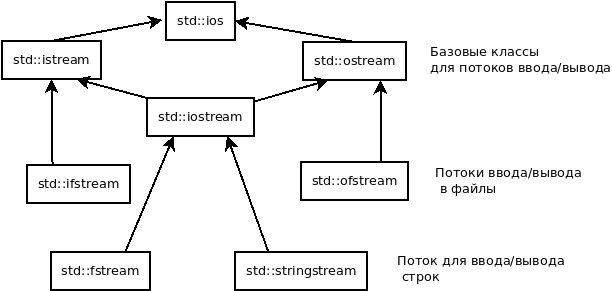
\includegraphics[width=0.8\textwidth]{io_classes.png}
\end{center}

Глобальные переенные \texttt{cin} (istream), \texttt{cout} (ostream), \texttt{cerr} (ostream).

Стандартная библиотека содержит перегруженные операторы \texttt{operator >>}, \texttt{operator <<} для примитивных типов и строк. 

\begin{minted}[fontsize=\footnotesize,numbersep=3pt,framesep=1mm,linenos,frame=single,label=]{cpp}
std::ostream& operator << (std::ostream& os, int v) {
    // convert int to bytes, write bytes
    return os;
}
\end{minted}
\begin{minted}[fontsize=\footnotesize,numbersep=3pt,framesep=1mm,linenos,frame=single,label=]{cpp}
std::istream& operator >> (std::istream& is, int& v) {
    // read bytes, convert to int
    return is;
}
\end{minted}
Такой код приводит к очистке буфера fflush потока, что замедляет вывод:
\begin{minted}[fontsize=\footnotesize,numbersep=3pt,framesep=1mm,linenos,frame=single,label=]{cpp}
std::cout << x << std::endl;
\end{minted}
Оператор читает строку до пробела, getline до конца строки:
\begin{minted}[fontsize=\footnotesize,numbersep=3pt,framesep=1mm,linenos,frame=single,label=]{cpp}
std::ifstream ifstream if("in.txt");
std::string word;
if >> word;
std::string line;
getline(if, line);
\end{minted}
Побайтовый ввод/вывод: read, write, seekg, tellg.

\subsection{Обработка ошибок}
rdstate() --- чем закончиласть последняя операция: eofbit, goodbit, failbit (считываем другим типом), badbit (не существует файла)
\subsection{Формат вывода}
\begin{minted}[fontsize=\footnotesize,numbersep=3pt,framesep=1mm,linenos,frame=single,label=]{cpp}
int x = 255;
std::cout.setf(std::ios::hex, std::ios::basefield);
std::cout << x; // после вывода флаг очистится
\end{minted}
Через манипуляторы
\begin{minted}[fontsize=\footnotesize,numbersep=3pt,framesep=1mm,linenos,frame=single,label=]{cpp}
ostream& operator << (ostream& (*pf)(ostream&));
\end{minted}
\subsection{Ввод-вывод пользовательских типов}
\begin{minted}[fontsize=\footnotesize,numbersep=3pt,framesep=1mm,linenos,frame=single,label=]{cpp}
class Point {
private:
    int x;
    int y;
public:
    friend ostream& operator << (ostream& os, const Point& p);
    friend istream& operator << (istream& is, Point& p);
    // friend функция может иметь доступ к приватным членам
};

ostream& operator << (ostream& os, const Point& p) {
    os << p.x << " " << p.y << "\n";
    return os;
}
istream& operator << (istream& is, Point& p) {
    is >> p.x >> p.y;
    return is;
}
\end{minted}
Так как ostream --- базовый класс, можно использовать один и тот же оператор для вывода на экран, строку и файл:
(cout, ofstream of("file"), stringstream ss).

 
\newpage % \documentclass[11pt,dvipsnames]{report}
% \usepackage[utf8]{inputenc}
% \usepackage[T2A]{fontenc}
\usepackage[english, russian]{babel}
% \usepackage{eufrak}
\usepackage{xltxtra}
\usepackage{polyglossia}
\usepackage{mathpazo}
\usepackage{fontspec}

\defaultfontfeatures{Ligatures=TeX,Mapping=tex-text}

\setmainfont[
ExternalLocation={/home/vyacheslav/builds/STIXv2.0.2/OTF/},
BoldFont=STIX2Text-Bold.otf,
ItalicFont=STIX2Text-Italic.otf,
BoldItalicFont=STIX2Text-BoldItalic.otf
]
{STIX2Text-Regular.otf}
\setmathrm{STIX2Math.otf}[
ExternalLocation={/home/vyacheslav/builds/STIXv2.0.2/OTF/}
]

\usepackage{amssymb, amsthm}
\usepackage{amsmath}
\usepackage{mathtools}
\usepackage{needspace}
\usepackage{enumitem}
\usepackage{cancel}
\usepackage{fdsymbol}

% разметка страницы и колонтитул
\usepackage[left=2cm,right=2cm,top=1.5cm,bottom=1cm,bindingoffset=0cm]{geometry}
\usepackage{fancybox,fancyhdr}
\fancyhf{}
\fancyhead[R]{\thepage}
\fancyhead[L]{\rightmark}
% \fancyfoot[RO,LE]{\thesection}
\fancyfoot[C]{\leftmark}
\addtolength{\headheight}{13pt}

\pagestyle{fancy}

% Отступы
\setlength{\parindent}{3ex}
\setlength{\parskip}{3pt}

\usepackage{graphicx}
\usepackage{hyperref}
\usepackage{epstopdf}

\usepackage{import}
\usepackage{xifthen}
\usepackage{pdfpages}
\usepackage{transparent}

\newcommand{\incfig}[1]{%
    \def\svgwidth{\columnwidth}
    \import{./figures/}{#1.pdf_tex}
}

\usepackage{xifthen}
\makeatother
\def\@lecture{}%
\newcommand{\lecture}[3]{
    \ifthenelse{\isempty{#3}}{%
        \def\@lecture{Лекция #1}%
    }{%
        \def\@lecture{Лекция #1: #3}%
    }%
    \subsection*{\@lecture}
    \marginpar{\small\textsf{\mbox{#2}}}
}
\makeatletter

\usepackage{xcolor}
\definecolor{Aquamarine}{cmyk}{50, 0, 17, 100}
\definecolor{ForestGreen}{cmyk}{76, 0, 76, 45}
\definecolor{Pink}{cmyk}{0, 100, 0, 0}
\definecolor{Cyan}{cmyk}{56, 0, 0, 100}
\definecolor{Gray}{gray}{0.3}

\newcommand{\Cclass}{\mathcal{C}}
\newcommand{\Dclass}{\mathcal{D}}
\newcommand{\K}{\mathcal{K}}
\newcommand{\Z}{\mathbb{Z}}
\newcommand{\N}{\mathbb{N}}
\newcommand{\Real}{\mathbb{R}}
\newcommand{\Q}{\mathbb{Q}}
\newcommand{\Cm}{\mathbb{C}}
\newcommand{\Pm}{\mathbb{P}}
\newcommand{\ord}{\operatorname{ord}}
\newcommand{\lcm}{\operatorname{lcm}}
\newcommand{\sign}{\operatorname{sign}}

\renewcommand{\o}{o}
\renewcommand{\O}{\mathcal{O}}
\renewcommand{\le}{\leqslant}
\renewcommand{\ge}{\geqslant}

\def\mybf#1{\textbf{#1}}
\def\selectedFont#1{\textbf{#1}}
% \def\mybf#1{{\usefont{T2A}{cmr}{m}{n}\textbf{#1}}}

% \usefont{T2A}{lmr}{m}{n}
% \usepackage{gentium}
% \usepackage{CormorantGaramond}

\usepackage{mdframed}
\mdfsetup{skipabove=3pt,skipbelow=3pt}
\mdfdefinestyle{defstyle}{%
    linecolor=red,
	linewidth=3pt,rightline=false,topline=false,bottomline=false,%
    frametitlerule=false,%
    frametitlebackgroundcolor=red!0,%
    innertopmargin=4pt,innerbottommargin=4pt,innerleftmargin=7pt
    frametitlebelowskip=1pt,
    frametitleaboveskip=3pt,
}
\mdfdefinestyle{thmstyle}{%
    linecolor=cyan!100,
	linewidth=2pt,topline=false,bottomline=false,%
    frametitlerule=false,%
    frametitlebackgroundcolor=cyan!20,%
    innertopmargin=4pt,innerbottommargin=4pt,
    frametitlebelowskip=1pt,
    frametitleaboveskip=3pt,
}
\theoremstyle{definition}
\mdtheorem[style=defstyle]{defn}{Определение}

\newmdtheoremenv[nobreak=true,backgroundcolor=Aquamarine!10,linewidth=0pt,innertopmargin=0pt,innerbottommargin=7pt]{cor}{Следствие}
\newmdtheoremenv[nobreak=true,backgroundcolor=CarnationPink!20,linewidth=0pt,innertopmargin=0pt,innerbottommargin=7pt]{desc}{Описание}
\newmdtheoremenv[nobreak=true,backgroundcolor=Gray!10,linewidth=0pt,innertopmargin=0pt,innerbottommargin=7pt,font={\small}]{ex}{Пример}
% \mdtheorem[style=thmstyle]{thm}{Теорема}
\newmdtheoremenv[nobreak=false,backgroundcolor=Cyan!10,linewidth=0pt,innertopmargin=0pt,innerbottommargin=7pt]{thm}{Теорема}
\newmdtheoremenv[nobreak=true,backgroundcolor=Pink!10,linewidth=0pt,innertopmargin=0pt,innerbottommargin=7pt]{lm}{Лемма}

\theoremstyle{plain}
\newtheorem*{st}{Утверждение}
\newtheorem*{prop}{Свойства}

\theoremstyle{definition}
\newtheorem*{name}{Обозначение}

\theoremstyle{remark}
\newtheorem*{rem}{Ремарка}
\newtheorem*{com}{Комментарий}
\newtheorem*{note}{Замечание}
\newtheorem*{prac}{Упражнение}
\newtheorem*{probl}{Задача}

\usepackage{fontawesome}
\renewcommand{\proofname}{Доказательство}
\renewenvironment{proof}
{ \small \hspace{\stretch{1}}\\ \faSquareO\quad  }
{ \hspace{\stretch{1}}  \faSquare \normalsize }

%{\fontsize{50}{60}\selectfont \faLinux}

\numberwithin{ex}{section}
\numberwithin{thm}{section}
\numberwithin{equation}{section}

\def\ComplexityFont#1{\textmd{\textbf{\textsf{#1}}}}
\renewcommand{\P}{\ComplexityFont{P}}
\newcommand{\DTIME}{\ComplexityFont{Dtime}}
\newcommand{\DSpace}{\ComplexityFont{DSpace}}
\newcommand{\PSPACE}{\ComplexityFont{PSPACE}}
\newcommand{\NTIME}{\ComplexityFont{Ntime}}
\newcommand{\SAT}{\ComplexityFont{SAT}}
\newcommand{\poly}{\ComplexityFont{poly}}
\newcommand{\FACTOR}{\ComplexityFont{FACTOR}}
\newcommand{\NP}{\ComplexityFont{NP}}
\newcommand{\NPcomp}{\ComplexityFont{NP-complete}}
\newcommand{\BH}{\ComplexityFont{BH}}
\newcommand{\tP}{\widetilde{\P}}
\newcommand{\tNP}{\widetilde{\NP}}
\newcommand{\tBH}{\widetilde{\BH}}
\newcommand{\UNSAT}{{\ComplexityFont{UNSAT}}}
\newcommand{\Class}{{\ComplexityFont{C}}}
\newcommand{\CircuitSat}{{\ComplexityFont{CIRCUIT\_SAT}}}
\newcommand{\tCircuitSat}{\widetilde{{\ComplexityFont{CIRCUIT\_SAT}}}}
\newcommand{\tSAT}{\widetilde{{\ComplexityFont{SAT}}}}
\newcommand{\tThreeSAT}{\widetilde{{\ComplexityFont{3\text{-}SAT}}}}
\newcommand{\ThreeSAT}{{\ComplexityFont{3\text{-}SAT}}}
\newcommand{\kQBF}{{\ComplexityFont{QBF{\tiny k}}}}
\newcommand{\QBFk}{{\ComplexityFont{QBF{\tiny k}}}}
\newcommand{\QBF}{{\ComplexityFont{QBF}}}
\newcommand{\coC}{\ComplexityFont{co-}\mathcal{C}}
\newcommand{\coNP}{\ComplexityFont{co-NP}}
\newcommand{\PH}{\ComplexityFont{PH}}
\newcommand{\EXP}{\ComplexityFont{EXP}}
\newcommand{\Size}{\ComplexityFont{Size}}
\newcommand{\Ppoly}{\ComplexityFont{P}/\ComplexityFont{poly}}

\newcommand{\const}{\textmd{const}}

\usepackage{ upgreek }
\newcommand{\PI}{\Uppi}
\newcommand{\SIGMA}{\Upsigma}
\newcommand{\DELTA}{\Updelta}


% \begin{document}
\section{Подгруппы циклических подгрупп. Прообраз подгрупп.}
\begin{thm}
    Пусть $G $ циклическая и $ H < G$. Тогда  $ H$ тоже циклическая.\\ Более того, если $ \left| G \right|  = n$,  то $ \forall d ~ n \del d\colon \exists! H \le \Z/n\colon \left| H \right| = d$. 
\end{thm}
\begin{myproof*}
    Рассмотрим два случая.
    \begin{itemize}
	\item $ G\simeq  \Z$.
	    \begin{lm}
	        Пусть $ H$ --- подгруппа в  $ \Z$. Тогда  $H $ циклическая.
	    \end{lm}
	\item $  G \simeq \Z / n$. Рассмотрим гомоморфизм, $ \pi\colon \Z \to  \Z / n$, $ \pi(x) = \overline{x}$.
	    \begin{lm}
		Пусть $ f\colon G_1 \to  G_2$ --- гомоморфизм групп, $ H \le G_2$. Тогда $ f^{-1}(H) \le G_1$.
	    \end{lm}
	    Мы знаем, что $ H \le G = \Z /n$. По прошлой лемме $ \pi^{-1}(H) \le \Z$, поэтому $ \pi^{-1}(H)$ циклическая. Из этого следует, что и $ H$ циклическая.

	    Докажем существование и единственность подгруппы порядка  $ d$, если  $ n \del d$. Рассмотрим элемент   $ \frac{n}{d} \in  \Z /n$, его порядок равен $ d$, поэтому порожденная им группа будет иметь такой же порядок.

	    Пусть  $ H = \langle x \rangle, ~ \ord x = d$. Если отождествить этот элемент с числом,  $ d = \frac{n}{(n, x)}$. Тогда $ \frac{n}{d} = (n, x) \Longrightarrow x \del \frac{n}{d} \Longrightarrow  H \subseteq \langle \frac{n}{d} \rangle$. Кроме этого в обоих группах $ d$ элементов, следовательно, они совпали.
    \end{itemize}
\end{myproof*}
% \end{document}
 
\newpage % \documentclass[11pt,dvipsnames,a4paper]{report}
% \usepackage[utf8]{inputenc}
% \usepackage[T2A]{fontenc}
\usepackage[english, russian]{babel}
% \usepackage{eufrak}
\usepackage{xltxtra}
\usepackage{polyglossia}
\usepackage{mathpazo}
\usepackage{fontspec}

\defaultfontfeatures{Ligatures=TeX,Mapping=tex-text}

\setmainfont[
ExternalLocation={/home/vyacheslav/builds/STIXv2.0.2/OTF/},
BoldFont=STIX2Text-Bold.otf,
ItalicFont=STIX2Text-Italic.otf,
BoldItalicFont=STIX2Text-BoldItalic.otf
]
{STIX2Text-Regular.otf}
\setmathrm{STIX2Math.otf}[
ExternalLocation={/home/vyacheslav/builds/STIXv2.0.2/OTF/}
]

\usepackage{amssymb, amsthm}
\usepackage{amsmath}
\usepackage{mathtools}
\usepackage{needspace}
\usepackage{enumitem}
\usepackage{cancel}
\usepackage{fdsymbol}

% разметка страницы и колонтитул
\usepackage[left=2cm,right=2cm,top=1.5cm,bottom=1cm,bindingoffset=0cm]{geometry}
\usepackage{fancybox,fancyhdr}
\fancyhf{}
\fancyhead[R]{\thepage}
\fancyhead[L]{\rightmark}
% \fancyfoot[RO,LE]{\thesection}
\fancyfoot[C]{\leftmark}
\addtolength{\headheight}{13pt}

\pagestyle{fancy}

% Отступы
\setlength{\parindent}{3ex}
\setlength{\parskip}{3pt}

\usepackage{graphicx}
\usepackage{hyperref}
\usepackage{epstopdf}

\usepackage{import}
\usepackage{xifthen}
\usepackage{pdfpages}
\usepackage{transparent}

\newcommand{\incfig}[1]{%
    \def\svgwidth{\columnwidth}
    \import{./figures/}{#1.pdf_tex}
}

\usepackage{xifthen}
\makeatother
\def\@lecture{}%
\newcommand{\lecture}[3]{
    \ifthenelse{\isempty{#3}}{%
        \def\@lecture{Лекция #1}%
    }{%
        \def\@lecture{Лекция #1: #3}%
    }%
    \subsection*{\@lecture}
    \marginpar{\small\textsf{\mbox{#2}}}
}
\makeatletter

\usepackage{xcolor}
\definecolor{Aquamarine}{cmyk}{50, 0, 17, 100}
\definecolor{ForestGreen}{cmyk}{76, 0, 76, 45}
\definecolor{Pink}{cmyk}{0, 100, 0, 0}
\definecolor{Cyan}{cmyk}{56, 0, 0, 100}
\definecolor{Gray}{gray}{0.3}

\newcommand{\Cclass}{\mathcal{C}}
\newcommand{\Dclass}{\mathcal{D}}
\newcommand{\K}{\mathcal{K}}
\newcommand{\Z}{\mathbb{Z}}
\newcommand{\N}{\mathbb{N}}
\newcommand{\Real}{\mathbb{R}}
\newcommand{\Q}{\mathbb{Q}}
\newcommand{\Cm}{\mathbb{C}}
\newcommand{\Pm}{\mathbb{P}}
\newcommand{\ord}{\operatorname{ord}}
\newcommand{\lcm}{\operatorname{lcm}}
\newcommand{\sign}{\operatorname{sign}}

\renewcommand{\o}{o}
\renewcommand{\O}{\mathcal{O}}
\renewcommand{\le}{\leqslant}
\renewcommand{\ge}{\geqslant}

\def\mybf#1{\textbf{#1}}
\def\selectedFont#1{\textbf{#1}}
% \def\mybf#1{{\usefont{T2A}{cmr}{m}{n}\textbf{#1}}}

% \usefont{T2A}{lmr}{m}{n}
% \usepackage{gentium}
% \usepackage{CormorantGaramond}

\usepackage{mdframed}
\mdfsetup{skipabove=3pt,skipbelow=3pt}
\mdfdefinestyle{defstyle}{%
    linecolor=red,
	linewidth=3pt,rightline=false,topline=false,bottomline=false,%
    frametitlerule=false,%
    frametitlebackgroundcolor=red!0,%
    innertopmargin=4pt,innerbottommargin=4pt,innerleftmargin=7pt
    frametitlebelowskip=1pt,
    frametitleaboveskip=3pt,
}
\mdfdefinestyle{thmstyle}{%
    linecolor=cyan!100,
	linewidth=2pt,topline=false,bottomline=false,%
    frametitlerule=false,%
    frametitlebackgroundcolor=cyan!20,%
    innertopmargin=4pt,innerbottommargin=4pt,
    frametitlebelowskip=1pt,
    frametitleaboveskip=3pt,
}
\theoremstyle{definition}
\mdtheorem[style=defstyle]{defn}{Определение}

\newmdtheoremenv[nobreak=true,backgroundcolor=Aquamarine!10,linewidth=0pt,innertopmargin=0pt,innerbottommargin=7pt]{cor}{Следствие}
\newmdtheoremenv[nobreak=true,backgroundcolor=CarnationPink!20,linewidth=0pt,innertopmargin=0pt,innerbottommargin=7pt]{desc}{Описание}
\newmdtheoremenv[nobreak=true,backgroundcolor=Gray!10,linewidth=0pt,innertopmargin=0pt,innerbottommargin=7pt,font={\small}]{ex}{Пример}
% \mdtheorem[style=thmstyle]{thm}{Теорема}
\newmdtheoremenv[nobreak=false,backgroundcolor=Cyan!10,linewidth=0pt,innertopmargin=0pt,innerbottommargin=7pt]{thm}{Теорема}
\newmdtheoremenv[nobreak=true,backgroundcolor=Pink!10,linewidth=0pt,innertopmargin=0pt,innerbottommargin=7pt]{lm}{Лемма}

\theoremstyle{plain}
\newtheorem*{st}{Утверждение}
\newtheorem*{prop}{Свойства}

\theoremstyle{definition}
\newtheorem*{name}{Обозначение}

\theoremstyle{remark}
\newtheorem*{rem}{Ремарка}
\newtheorem*{com}{Комментарий}
\newtheorem*{note}{Замечание}
\newtheorem*{prac}{Упражнение}
\newtheorem*{probl}{Задача}

\usepackage{fontawesome}
\renewcommand{\proofname}{Доказательство}
\renewenvironment{proof}
{ \small \hspace{\stretch{1}}\\ \faSquareO\quad  }
{ \hspace{\stretch{1}}  \faSquare \normalsize }

%{\fontsize{50}{60}\selectfont \faLinux}

\numberwithin{ex}{section}
\numberwithin{thm}{section}
\numberwithin{equation}{section}

\def\ComplexityFont#1{\textmd{\textbf{\textsf{#1}}}}
\renewcommand{\P}{\ComplexityFont{P}}
\newcommand{\DTIME}{\ComplexityFont{Dtime}}
\newcommand{\DSpace}{\ComplexityFont{DSpace}}
\newcommand{\PSPACE}{\ComplexityFont{PSPACE}}
\newcommand{\NTIME}{\ComplexityFont{Ntime}}
\newcommand{\SAT}{\ComplexityFont{SAT}}
\newcommand{\poly}{\ComplexityFont{poly}}
\newcommand{\FACTOR}{\ComplexityFont{FACTOR}}
\newcommand{\NP}{\ComplexityFont{NP}}
\newcommand{\NPcomp}{\ComplexityFont{NP-complete}}
\newcommand{\BH}{\ComplexityFont{BH}}
\newcommand{\tP}{\widetilde{\P}}
\newcommand{\tNP}{\widetilde{\NP}}
\newcommand{\tBH}{\widetilde{\BH}}
\newcommand{\UNSAT}{{\ComplexityFont{UNSAT}}}
\newcommand{\Class}{{\ComplexityFont{C}}}
\newcommand{\CircuitSat}{{\ComplexityFont{CIRCUIT\_SAT}}}
\newcommand{\tCircuitSat}{\widetilde{{\ComplexityFont{CIRCUIT\_SAT}}}}
\newcommand{\tSAT}{\widetilde{{\ComplexityFont{SAT}}}}
\newcommand{\tThreeSAT}{\widetilde{{\ComplexityFont{3\text{-}SAT}}}}
\newcommand{\ThreeSAT}{{\ComplexityFont{3\text{-}SAT}}}
\newcommand{\kQBF}{{\ComplexityFont{QBF{\tiny k}}}}
\newcommand{\QBFk}{{\ComplexityFont{QBF{\tiny k}}}}
\newcommand{\QBF}{{\ComplexityFont{QBF}}}
\newcommand{\coC}{\ComplexityFont{co-}\mathcal{C}}
\newcommand{\coNP}{\ComplexityFont{co-NP}}
\newcommand{\PH}{\ComplexityFont{PH}}
\newcommand{\EXP}{\ComplexityFont{EXP}}
\newcommand{\Size}{\ComplexityFont{Size}}
\newcommand{\Ppoly}{\ComplexityFont{P}/\ComplexityFont{poly}}

\newcommand{\const}{\textmd{const}}

\usepackage{ upgreek }
\newcommand{\PI}{\Uppi}
\newcommand{\SIGMA}{\Upsigma}
\newcommand{\DELTA}{\Updelta}


% \begin{document}
\section{Структуры. Интрузивный связный список на C}
\begin{itemize}[noitemsep]
    \item интрузивная реализация
    \item typedef
\end{itemize}
\subsection{Интрузивная реализация}
Такой список хранит интрузивные вершины, внутри которых лежат вершины с данными. Внутренние блоки не имеют связи между собой. За счет этого мы можем создать один список и использовать его для разных типов.
\begin{ccode}
#include <stdlib.h>

struct IntrusiveNode {
    struct IntrusiveNode *next;
    struct IntrusiveNode *prev;
};

struct IntrusiveList {
    struct IntrusiveNode *head;
};

struct Node {
    int data;
    struct IntrusiveNode *node;
};

void add_intr_node(struct IntrusiveList *list, struct IntrusiveNode *new_node) {
    new_node->prev = list->head;
    new_node->next = list->head->next;
    new_node->next->prev = new_node;
    list->head->next = new_node;
}

void add_node(struct IntrusiveList *list, int data) {
    struct Node *new_node = malloc(sizeof(struct Node));
    struct IntrusiveNode *new_intr_node = malloc(sizeof(struct IntrusiveNode));
    new_node->data = data;
    new_node->node = new_intr_node;
    add_intr_node(list, new_intr_node); 
}

void delete_node(struct IntrusiveList *list, struct Node *dnode) {
    struct IntrusiveNode *intr_node = dnode->node;
    intr_node->prev->next = intr_node->next;
    intr_node->next->prev = intr_node->prev;
    free(dnode); free(intr_node);
}
\end{ccode}
\subsection{typedef}
Не команда для препроцессора, это просто синоним для существующего типа.
\begin{ccode}
typedef long long ll;
typedef struct point {
    //pass
} point_s
\end{ccode}
% \end{document}
 
\newpage \section{Формула для обратной матрицы. Присоединенная матрица. Соотношение для присоединенной матрицы.}
\begin{defn}[Присоединенная матрица]
{\sf Присоединенная матрица} к матрице $ A$ --- матрица $ (\Adj A)_{ij} = A^{ij}$, где $ A^{ij}$ --- алгебраическое дополнение элемента $ a_{ij}$.   
\end{defn}
\begin{thm}
    Пусть $ A \in M_n(K)$. Тогда 
    $
	\Adj A \cdot A = A \cdot \Adj A = \det( A) \cdot E
	$.
\end{thm}
 
\newpage % \documentclass[11pt,dvipsnames]{report}
% \usepackage[utf8]{inputenc}
% \usepackage[T2A]{fontenc}
\usepackage[english, russian]{babel}
% \usepackage{eufrak}
\usepackage{xltxtra}
\usepackage{polyglossia}
\usepackage{mathpazo}
\usepackage{fontspec}

\defaultfontfeatures{Ligatures=TeX,Mapping=tex-text}

\setmainfont[
ExternalLocation={/home/vyacheslav/builds/STIXv2.0.2/OTF/},
BoldFont=STIX2Text-Bold.otf,
ItalicFont=STIX2Text-Italic.otf,
BoldItalicFont=STIX2Text-BoldItalic.otf
]
{STIX2Text-Regular.otf}
\setmathrm{STIX2Math.otf}[
ExternalLocation={/home/vyacheslav/builds/STIXv2.0.2/OTF/}
]

\usepackage{amssymb, amsthm}
\usepackage{amsmath}
\usepackage{mathtools}
\usepackage{needspace}
\usepackage{enumitem}
\usepackage{cancel}
\usepackage{fdsymbol}

% разметка страницы и колонтитул
\usepackage[left=2cm,right=2cm,top=1.5cm,bottom=1cm,bindingoffset=0cm]{geometry}
\usepackage{fancybox,fancyhdr}
\fancyhf{}
\fancyhead[R]{\thepage}
\fancyhead[L]{\rightmark}
% \fancyfoot[RO,LE]{\thesection}
\fancyfoot[C]{\leftmark}
\addtolength{\headheight}{13pt}

\pagestyle{fancy}

% Отступы
\setlength{\parindent}{3ex}
\setlength{\parskip}{3pt}

\usepackage{graphicx}
\usepackage{hyperref}
\usepackage{epstopdf}

\usepackage{import}
\usepackage{xifthen}
\usepackage{pdfpages}
\usepackage{transparent}

\newcommand{\incfig}[1]{%
    \def\svgwidth{\columnwidth}
    \import{./figures/}{#1.pdf_tex}
}

\usepackage{xifthen}
\makeatother
\def\@lecture{}%
\newcommand{\lecture}[3]{
    \ifthenelse{\isempty{#3}}{%
        \def\@lecture{Лекция #1}%
    }{%
        \def\@lecture{Лекция #1: #3}%
    }%
    \subsection*{\@lecture}
    \marginpar{\small\textsf{\mbox{#2}}}
}
\makeatletter

\usepackage{xcolor}
\definecolor{Aquamarine}{cmyk}{50, 0, 17, 100}
\definecolor{ForestGreen}{cmyk}{76, 0, 76, 45}
\definecolor{Pink}{cmyk}{0, 100, 0, 0}
\definecolor{Cyan}{cmyk}{56, 0, 0, 100}
\definecolor{Gray}{gray}{0.3}

\newcommand{\Cclass}{\mathcal{C}}
\newcommand{\Dclass}{\mathcal{D}}
\newcommand{\K}{\mathcal{K}}
\newcommand{\Z}{\mathbb{Z}}
\newcommand{\N}{\mathbb{N}}
\newcommand{\Real}{\mathbb{R}}
\newcommand{\Q}{\mathbb{Q}}
\newcommand{\Cm}{\mathbb{C}}
\newcommand{\Pm}{\mathbb{P}}
\newcommand{\ord}{\operatorname{ord}}
\newcommand{\lcm}{\operatorname{lcm}}
\newcommand{\sign}{\operatorname{sign}}

\renewcommand{\o}{o}
\renewcommand{\O}{\mathcal{O}}
\renewcommand{\le}{\leqslant}
\renewcommand{\ge}{\geqslant}

\def\mybf#1{\textbf{#1}}
\def\selectedFont#1{\textbf{#1}}
% \def\mybf#1{{\usefont{T2A}{cmr}{m}{n}\textbf{#1}}}

% \usefont{T2A}{lmr}{m}{n}
% \usepackage{gentium}
% \usepackage{CormorantGaramond}

\usepackage{mdframed}
\mdfsetup{skipabove=3pt,skipbelow=3pt}
\mdfdefinestyle{defstyle}{%
    linecolor=red,
	linewidth=3pt,rightline=false,topline=false,bottomline=false,%
    frametitlerule=false,%
    frametitlebackgroundcolor=red!0,%
    innertopmargin=4pt,innerbottommargin=4pt,innerleftmargin=7pt
    frametitlebelowskip=1pt,
    frametitleaboveskip=3pt,
}
\mdfdefinestyle{thmstyle}{%
    linecolor=cyan!100,
	linewidth=2pt,topline=false,bottomline=false,%
    frametitlerule=false,%
    frametitlebackgroundcolor=cyan!20,%
    innertopmargin=4pt,innerbottommargin=4pt,
    frametitlebelowskip=1pt,
    frametitleaboveskip=3pt,
}
\theoremstyle{definition}
\mdtheorem[style=defstyle]{defn}{Определение}

\newmdtheoremenv[nobreak=true,backgroundcolor=Aquamarine!10,linewidth=0pt,innertopmargin=0pt,innerbottommargin=7pt]{cor}{Следствие}
\newmdtheoremenv[nobreak=true,backgroundcolor=CarnationPink!20,linewidth=0pt,innertopmargin=0pt,innerbottommargin=7pt]{desc}{Описание}
\newmdtheoremenv[nobreak=true,backgroundcolor=Gray!10,linewidth=0pt,innertopmargin=0pt,innerbottommargin=7pt,font={\small}]{ex}{Пример}
% \mdtheorem[style=thmstyle]{thm}{Теорема}
\newmdtheoremenv[nobreak=false,backgroundcolor=Cyan!10,linewidth=0pt,innertopmargin=0pt,innerbottommargin=7pt]{thm}{Теорема}
\newmdtheoremenv[nobreak=true,backgroundcolor=Pink!10,linewidth=0pt,innertopmargin=0pt,innerbottommargin=7pt]{lm}{Лемма}

\theoremstyle{plain}
\newtheorem*{st}{Утверждение}
\newtheorem*{prop}{Свойства}

\theoremstyle{definition}
\newtheorem*{name}{Обозначение}

\theoremstyle{remark}
\newtheorem*{rem}{Ремарка}
\newtheorem*{com}{Комментарий}
\newtheorem*{note}{Замечание}
\newtheorem*{prac}{Упражнение}
\newtheorem*{probl}{Задача}

\usepackage{fontawesome}
\renewcommand{\proofname}{Доказательство}
\renewenvironment{proof}
{ \small \hspace{\stretch{1}}\\ \faSquareO\quad  }
{ \hspace{\stretch{1}}  \faSquare \normalsize }

%{\fontsize{50}{60}\selectfont \faLinux}

\numberwithin{ex}{section}
\numberwithin{thm}{section}
\numberwithin{equation}{section}

\def\ComplexityFont#1{\textmd{\textbf{\textsf{#1}}}}
\renewcommand{\P}{\ComplexityFont{P}}
\newcommand{\DTIME}{\ComplexityFont{Dtime}}
\newcommand{\DSpace}{\ComplexityFont{DSpace}}
\newcommand{\PSPACE}{\ComplexityFont{PSPACE}}
\newcommand{\NTIME}{\ComplexityFont{Ntime}}
\newcommand{\SAT}{\ComplexityFont{SAT}}
\newcommand{\poly}{\ComplexityFont{poly}}
\newcommand{\FACTOR}{\ComplexityFont{FACTOR}}
\newcommand{\NP}{\ComplexityFont{NP}}
\newcommand{\NPcomp}{\ComplexityFont{NP-complete}}
\newcommand{\BH}{\ComplexityFont{BH}}
\newcommand{\tP}{\widetilde{\P}}
\newcommand{\tNP}{\widetilde{\NP}}
\newcommand{\tBH}{\widetilde{\BH}}
\newcommand{\UNSAT}{{\ComplexityFont{UNSAT}}}
\newcommand{\Class}{{\ComplexityFont{C}}}
\newcommand{\CircuitSat}{{\ComplexityFont{CIRCUIT\_SAT}}}
\newcommand{\tCircuitSat}{\widetilde{{\ComplexityFont{CIRCUIT\_SAT}}}}
\newcommand{\tSAT}{\widetilde{{\ComplexityFont{SAT}}}}
\newcommand{\tThreeSAT}{\widetilde{{\ComplexityFont{3\text{-}SAT}}}}
\newcommand{\ThreeSAT}{{\ComplexityFont{3\text{-}SAT}}}
\newcommand{\kQBF}{{\ComplexityFont{QBF{\tiny k}}}}
\newcommand{\QBFk}{{\ComplexityFont{QBF{\tiny k}}}}
\newcommand{\QBF}{{\ComplexityFont{QBF}}}
\newcommand{\coC}{\ComplexityFont{co-}\mathcal{C}}
\newcommand{\coNP}{\ComplexityFont{co-NP}}
\newcommand{\PH}{\ComplexityFont{PH}}
\newcommand{\EXP}{\ComplexityFont{EXP}}
\newcommand{\Size}{\ComplexityFont{Size}}
\newcommand{\Ppoly}{\ComplexityFont{P}/\ComplexityFont{poly}}

\newcommand{\const}{\textmd{const}}

\usepackage{ upgreek }
\newcommand{\PI}{\Uppi}
\newcommand{\SIGMA}{\Upsigma}
\newcommand{\DELTA}{\Updelta}


% \begin{document}
\section{Представление перестановки в виде произведения независимых циклов. Порядок перестановки. Обратная перестановка и ее циклическая запись.}
\begin{defn}[Цикл]
    Пусть  $ \{a_1, \ldots a_k\} \subset \{1, \ldots n\}$.
    {\sf Цикл} $ (a_1, \ldots , a_k)$ --- такой элемент $ c $ из  $ S_n$, что  
    \[
	c(x) =
	\begin{cases}
	    x, & x \not\in \{a_1, \ldots a_k\}\\
	    a_{i+1}, & x = a_i \wedge 1 \le i < k\\
	    a_1, & x = a_k
	\end{cases}
    .\] 
    \begin{note}
	Порядок $ (a_1, \ldots , a_k)$ равен $ k$.
    \end{note}
\end{defn}
\begin{defn}[Неподвижная точка]
    Пусть $ \sigma \in S_{n}$. {\sf Неподвижная точка} --- такой $ x \in \{1, \ldots , n\}$, что $ \sigma (x) = x$. 
    \begin{name}
	$ \Fix(\sigma ) $ --- множество всех неподвижных точек относительно $ \sigma $.  
    \end{name}
\end{defn}
\begin{defn}[Носитель]
    {\sf Носитель перестановки $ \sigma \in  S_{n} $} --- множество $ \{1, \ldots , n\} \setminus \Fix( \sigma )$.  
    \begin{name}
        $ \supp \sigma $.
    \end{name}
\end{defn}
\begin{defn}[Независимость перестановок]
    Перестановки $\sigma _1 , \sigma _2 \in S_{n} $ называются {\sf независимыми}, если $ \supp \sigma _1 \cap \supp \sigma _2 = \varnothing$.  
    \begin{prop}
        Две независимые перестановки коммутируют.
    \end{prop}
\end{defn}
\begin{thm}[Разложение в произведение циклов]
    Пусть $ \sigma \in S_{n} $. Тогда существует единственный с точностью до порядка набор независимых циклов $ c_1, \ldots , c_k, ~ c_i \ne \id$, что $ \sigma  = c_1  \ldots c_k$.
\end{thm}
\begin{thm}[Порядок перестановки]
    Пусть $ \sigma  \in S_n$ и $ \sigma  = c_1\ldots c_k$. Обозначим $ d_i$ за длину  $ c_i$. Тогда  $ \ord \sigma  = НОК\left( d_1, \ldots d_k \right) $
\end{thm}
\begin{thm}[Обратная перестановка в циклической записи]
    Пусть $ c = (a_1, \ldots a_k)$. Тогда $ c^{-1} = (a_k, \ldots a_1)$.\\ Если $ \sigma  = c_1c_2\ldots c_s$, где $ c_i$ --- независимые циклы, то  $ \sigma^{-1} = c_1^{-1}c_2^{-1}\ldots c_s^{-1}$.
\end{thm}
% \end{document}
 
\newpage \documentclass[11pt,dvipsnames]{report}
\usepackage[utf8]{inputenc}
% \usepackage[T2A]{fontenc}
\usepackage[english, russian]{babel}
% \usepackage{eufrak}
\usepackage{xltxtra}
\usepackage{polyglossia}
\usepackage{mathpazo}
\usepackage{fontspec}

\defaultfontfeatures{Ligatures=TeX,Mapping=tex-text}

\setmainfont[
ExternalLocation={/home/vyacheslav/builds/STIXv2.0.2/OTF/},
BoldFont=STIX2Text-Bold.otf,
ItalicFont=STIX2Text-Italic.otf,
BoldItalicFont=STIX2Text-BoldItalic.otf
]
{STIX2Text-Regular.otf}
\setmathrm{STIX2Math.otf}[
ExternalLocation={/home/vyacheslav/builds/STIXv2.0.2/OTF/}
]

\usepackage{amssymb, amsthm}
\usepackage{amsmath}
\usepackage{mathtools}
\usepackage{needspace}
\usepackage{enumitem}
\usepackage{cancel}
\usepackage{fdsymbol}

% разметка страницы и колонтитул
\usepackage[left=2cm,right=2cm,top=1.5cm,bottom=1cm,bindingoffset=0cm]{geometry}
\usepackage{fancybox,fancyhdr}
\fancyhf{}
\fancyhead[R]{\thepage}
\fancyhead[L]{\rightmark}
% \fancyfoot[RO,LE]{\thesection}
\fancyfoot[C]{\leftmark}
\addtolength{\headheight}{13pt}

\pagestyle{fancy}

% Отступы
\setlength{\parindent}{3ex}
\setlength{\parskip}{3pt}

\usepackage{graphicx}
\usepackage{hyperref}
\usepackage{epstopdf}

\usepackage{import}
\usepackage{xifthen}
\usepackage{pdfpages}
\usepackage{transparent}

\newcommand{\incfig}[1]{%
    \def\svgwidth{\columnwidth}
    \import{./figures/}{#1.pdf_tex}
}

\usepackage{xifthen}
\makeatother
\def\@lecture{}%
\newcommand{\lecture}[3]{
    \ifthenelse{\isempty{#3}}{%
        \def\@lecture{Лекция #1}%
    }{%
        \def\@lecture{Лекция #1: #3}%
    }%
    \subsection*{\@lecture}
    \marginpar{\small\textsf{\mbox{#2}}}
}
\makeatletter

\usepackage{xcolor}
\definecolor{Aquamarine}{cmyk}{50, 0, 17, 100}
\definecolor{ForestGreen}{cmyk}{76, 0, 76, 45}
\definecolor{Pink}{cmyk}{0, 100, 0, 0}
\definecolor{Cyan}{cmyk}{56, 0, 0, 100}
\definecolor{Gray}{gray}{0.3}

\newcommand{\Cclass}{\mathcal{C}}
\newcommand{\Dclass}{\mathcal{D}}
\newcommand{\K}{\mathcal{K}}
\newcommand{\Z}{\mathbb{Z}}
\newcommand{\N}{\mathbb{N}}
\newcommand{\Real}{\mathbb{R}}
\newcommand{\Q}{\mathbb{Q}}
\newcommand{\Cm}{\mathbb{C}}
\newcommand{\Pm}{\mathbb{P}}
\newcommand{\ord}{\operatorname{ord}}
\newcommand{\lcm}{\operatorname{lcm}}
\newcommand{\sign}{\operatorname{sign}}

\renewcommand{\o}{o}
\renewcommand{\O}{\mathcal{O}}
\renewcommand{\le}{\leqslant}
\renewcommand{\ge}{\geqslant}

\def\mybf#1{\textbf{#1}}
\def\selectedFont#1{\textbf{#1}}
% \def\mybf#1{{\usefont{T2A}{cmr}{m}{n}\textbf{#1}}}

% \usefont{T2A}{lmr}{m}{n}
% \usepackage{gentium}
% \usepackage{CormorantGaramond}

\usepackage{mdframed}
\mdfsetup{skipabove=3pt,skipbelow=3pt}
\mdfdefinestyle{defstyle}{%
    linecolor=red,
	linewidth=3pt,rightline=false,topline=false,bottomline=false,%
    frametitlerule=false,%
    frametitlebackgroundcolor=red!0,%
    innertopmargin=4pt,innerbottommargin=4pt,innerleftmargin=7pt
    frametitlebelowskip=1pt,
    frametitleaboveskip=3pt,
}
\mdfdefinestyle{thmstyle}{%
    linecolor=cyan!100,
	linewidth=2pt,topline=false,bottomline=false,%
    frametitlerule=false,%
    frametitlebackgroundcolor=cyan!20,%
    innertopmargin=4pt,innerbottommargin=4pt,
    frametitlebelowskip=1pt,
    frametitleaboveskip=3pt,
}
\theoremstyle{definition}
\mdtheorem[style=defstyle]{defn}{Определение}

\newmdtheoremenv[nobreak=true,backgroundcolor=Aquamarine!10,linewidth=0pt,innertopmargin=0pt,innerbottommargin=7pt]{cor}{Следствие}
\newmdtheoremenv[nobreak=true,backgroundcolor=CarnationPink!20,linewidth=0pt,innertopmargin=0pt,innerbottommargin=7pt]{desc}{Описание}
\newmdtheoremenv[nobreak=true,backgroundcolor=Gray!10,linewidth=0pt,innertopmargin=0pt,innerbottommargin=7pt,font={\small}]{ex}{Пример}
% \mdtheorem[style=thmstyle]{thm}{Теорема}
\newmdtheoremenv[nobreak=false,backgroundcolor=Cyan!10,linewidth=0pt,innertopmargin=0pt,innerbottommargin=7pt]{thm}{Теорема}
\newmdtheoremenv[nobreak=true,backgroundcolor=Pink!10,linewidth=0pt,innertopmargin=0pt,innerbottommargin=7pt]{lm}{Лемма}

\theoremstyle{plain}
\newtheorem*{st}{Утверждение}
\newtheorem*{prop}{Свойства}

\theoremstyle{definition}
\newtheorem*{name}{Обозначение}

\theoremstyle{remark}
\newtheorem*{rem}{Ремарка}
\newtheorem*{com}{Комментарий}
\newtheorem*{note}{Замечание}
\newtheorem*{prac}{Упражнение}
\newtheorem*{probl}{Задача}

\usepackage{fontawesome}
\renewcommand{\proofname}{Доказательство}
\renewenvironment{proof}
{ \small \hspace{\stretch{1}}\\ \faSquareO\quad  }
{ \hspace{\stretch{1}}  \faSquare \normalsize }

%{\fontsize{50}{60}\selectfont \faLinux}

\numberwithin{ex}{section}
\numberwithin{thm}{section}
\numberwithin{equation}{section}

\def\ComplexityFont#1{\textmd{\textbf{\textsf{#1}}}}
\renewcommand{\P}{\ComplexityFont{P}}
\newcommand{\DTIME}{\ComplexityFont{Dtime}}
\newcommand{\DSpace}{\ComplexityFont{DSpace}}
\newcommand{\PSPACE}{\ComplexityFont{PSPACE}}
\newcommand{\NTIME}{\ComplexityFont{Ntime}}
\newcommand{\SAT}{\ComplexityFont{SAT}}
\newcommand{\poly}{\ComplexityFont{poly}}
\newcommand{\FACTOR}{\ComplexityFont{FACTOR}}
\newcommand{\NP}{\ComplexityFont{NP}}
\newcommand{\NPcomp}{\ComplexityFont{NP-complete}}
\newcommand{\BH}{\ComplexityFont{BH}}
\newcommand{\tP}{\widetilde{\P}}
\newcommand{\tNP}{\widetilde{\NP}}
\newcommand{\tBH}{\widetilde{\BH}}
\newcommand{\UNSAT}{{\ComplexityFont{UNSAT}}}
\newcommand{\Class}{{\ComplexityFont{C}}}
\newcommand{\CircuitSat}{{\ComplexityFont{CIRCUIT\_SAT}}}
\newcommand{\tCircuitSat}{\widetilde{{\ComplexityFont{CIRCUIT\_SAT}}}}
\newcommand{\tSAT}{\widetilde{{\ComplexityFont{SAT}}}}
\newcommand{\tThreeSAT}{\widetilde{{\ComplexityFont{3\text{-}SAT}}}}
\newcommand{\ThreeSAT}{{\ComplexityFont{3\text{-}SAT}}}
\newcommand{\kQBF}{{\ComplexityFont{QBF{\tiny k}}}}
\newcommand{\QBFk}{{\ComplexityFont{QBF{\tiny k}}}}
\newcommand{\QBF}{{\ComplexityFont{QBF}}}
\newcommand{\coC}{\ComplexityFont{co-}\mathcal{C}}
\newcommand{\coNP}{\ComplexityFont{co-NP}}
\newcommand{\PH}{\ComplexityFont{PH}}
\newcommand{\EXP}{\ComplexityFont{EXP}}
\newcommand{\Size}{\ComplexityFont{Size}}
\newcommand{\Ppoly}{\ComplexityFont{P}/\ComplexityFont{poly}}

\newcommand{\const}{\textmd{const}}

\usepackage{ upgreek }
\newcommand{\PI}{\Uppi}
\newcommand{\SIGMA}{\Upsigma}
\newcommand{\DELTA}{\Updelta}


\begin{document}
\section{Разложение в произведение транспозиций. Знак перестановки. Знак как гомоморфизм. Знак и число транспозиций в разложении.}
\begin{defn}[Транспозиция]
    Цикл вида $ (ij), ~ i \ne j$ называется {\sf транспозицией}.  
\end{defn}
\begin{st}
    Любая перестановка раскладывается в произведение транспозиций.
\end{st}
\begin{defn}[Инверсия]
    Пара $ i < j$ образует  {\sf инверсию}, если $ \sigma (i) > \sigma (j)$.  
\end{defn}
\begin{defn}[Четность и знак перестановки]
    {\sf Четность перестановки} --- четность числа инверсий $ Inv(\sigma)$ в ней.  
    \\
    {\sf Знак перестановки} --- число
    \[
	\sgn( \sigma ) = (-1)^{Inv( \sigma )} = \prod_{i>j} \frac{ \sigma (i) - \sigma (j)}{i - j}
    .\] 
\end{defn}
\end{document}
 
\newpage % \documentclass[11pt,dvipsnames]{report}
% \usepackage[utf8]{inputenc}
% \usepackage[T2A]{fontenc}
\usepackage[english, russian]{babel}
% \usepackage{eufrak}
\usepackage{xltxtra}
\usepackage{polyglossia}
\usepackage{mathpazo}
\usepackage{fontspec}

\defaultfontfeatures{Ligatures=TeX,Mapping=tex-text}

\setmainfont[
ExternalLocation={/home/vyacheslav/builds/STIXv2.0.2/OTF/},
BoldFont=STIX2Text-Bold.otf,
ItalicFont=STIX2Text-Italic.otf,
BoldItalicFont=STIX2Text-BoldItalic.otf
]
{STIX2Text-Regular.otf}
\setmathrm{STIX2Math.otf}[
ExternalLocation={/home/vyacheslav/builds/STIXv2.0.2/OTF/}
]

\usepackage{amssymb, amsthm}
\usepackage{amsmath}
\usepackage{mathtools}
\usepackage{needspace}
\usepackage{enumitem}
\usepackage{cancel}
\usepackage{fdsymbol}

% разметка страницы и колонтитул
\usepackage[left=2cm,right=2cm,top=1.5cm,bottom=1cm,bindingoffset=0cm]{geometry}
\usepackage{fancybox,fancyhdr}
\fancyhf{}
\fancyhead[R]{\thepage}
\fancyhead[L]{\rightmark}
% \fancyfoot[RO,LE]{\thesection}
\fancyfoot[C]{\leftmark}
\addtolength{\headheight}{13pt}

\pagestyle{fancy}

% Отступы
\setlength{\parindent}{3ex}
\setlength{\parskip}{3pt}

\usepackage{graphicx}
\usepackage{hyperref}
\usepackage{epstopdf}

\usepackage{import}
\usepackage{xifthen}
\usepackage{pdfpages}
\usepackage{transparent}

\newcommand{\incfig}[1]{%
    \def\svgwidth{\columnwidth}
    \import{./figures/}{#1.pdf_tex}
}

\usepackage{xifthen}
\makeatother
\def\@lecture{}%
\newcommand{\lecture}[3]{
    \ifthenelse{\isempty{#3}}{%
        \def\@lecture{Лекция #1}%
    }{%
        \def\@lecture{Лекция #1: #3}%
    }%
    \subsection*{\@lecture}
    \marginpar{\small\textsf{\mbox{#2}}}
}
\makeatletter

\usepackage{xcolor}
\definecolor{Aquamarine}{cmyk}{50, 0, 17, 100}
\definecolor{ForestGreen}{cmyk}{76, 0, 76, 45}
\definecolor{Pink}{cmyk}{0, 100, 0, 0}
\definecolor{Cyan}{cmyk}{56, 0, 0, 100}
\definecolor{Gray}{gray}{0.3}

\newcommand{\Cclass}{\mathcal{C}}
\newcommand{\Dclass}{\mathcal{D}}
\newcommand{\K}{\mathcal{K}}
\newcommand{\Z}{\mathbb{Z}}
\newcommand{\N}{\mathbb{N}}
\newcommand{\Real}{\mathbb{R}}
\newcommand{\Q}{\mathbb{Q}}
\newcommand{\Cm}{\mathbb{C}}
\newcommand{\Pm}{\mathbb{P}}
\newcommand{\ord}{\operatorname{ord}}
\newcommand{\lcm}{\operatorname{lcm}}
\newcommand{\sign}{\operatorname{sign}}

\renewcommand{\o}{o}
\renewcommand{\O}{\mathcal{O}}
\renewcommand{\le}{\leqslant}
\renewcommand{\ge}{\geqslant}

\def\mybf#1{\textbf{#1}}
\def\selectedFont#1{\textbf{#1}}
% \def\mybf#1{{\usefont{T2A}{cmr}{m}{n}\textbf{#1}}}

% \usefont{T2A}{lmr}{m}{n}
% \usepackage{gentium}
% \usepackage{CormorantGaramond}

\usepackage{mdframed}
\mdfsetup{skipabove=3pt,skipbelow=3pt}
\mdfdefinestyle{defstyle}{%
    linecolor=red,
	linewidth=3pt,rightline=false,topline=false,bottomline=false,%
    frametitlerule=false,%
    frametitlebackgroundcolor=red!0,%
    innertopmargin=4pt,innerbottommargin=4pt,innerleftmargin=7pt
    frametitlebelowskip=1pt,
    frametitleaboveskip=3pt,
}
\mdfdefinestyle{thmstyle}{%
    linecolor=cyan!100,
	linewidth=2pt,topline=false,bottomline=false,%
    frametitlerule=false,%
    frametitlebackgroundcolor=cyan!20,%
    innertopmargin=4pt,innerbottommargin=4pt,
    frametitlebelowskip=1pt,
    frametitleaboveskip=3pt,
}
\theoremstyle{definition}
\mdtheorem[style=defstyle]{defn}{Определение}

\newmdtheoremenv[nobreak=true,backgroundcolor=Aquamarine!10,linewidth=0pt,innertopmargin=0pt,innerbottommargin=7pt]{cor}{Следствие}
\newmdtheoremenv[nobreak=true,backgroundcolor=CarnationPink!20,linewidth=0pt,innertopmargin=0pt,innerbottommargin=7pt]{desc}{Описание}
\newmdtheoremenv[nobreak=true,backgroundcolor=Gray!10,linewidth=0pt,innertopmargin=0pt,innerbottommargin=7pt,font={\small}]{ex}{Пример}
% \mdtheorem[style=thmstyle]{thm}{Теорема}
\newmdtheoremenv[nobreak=false,backgroundcolor=Cyan!10,linewidth=0pt,innertopmargin=0pt,innerbottommargin=7pt]{thm}{Теорема}
\newmdtheoremenv[nobreak=true,backgroundcolor=Pink!10,linewidth=0pt,innertopmargin=0pt,innerbottommargin=7pt]{lm}{Лемма}

\theoremstyle{plain}
\newtheorem*{st}{Утверждение}
\newtheorem*{prop}{Свойства}

\theoremstyle{definition}
\newtheorem*{name}{Обозначение}

\theoremstyle{remark}
\newtheorem*{rem}{Ремарка}
\newtheorem*{com}{Комментарий}
\newtheorem*{note}{Замечание}
\newtheorem*{prac}{Упражнение}
\newtheorem*{probl}{Задача}

\usepackage{fontawesome}
\renewcommand{\proofname}{Доказательство}
\renewenvironment{proof}
{ \small \hspace{\stretch{1}}\\ \faSquareO\quad  }
{ \hspace{\stretch{1}}  \faSquare \normalsize }

%{\fontsize{50}{60}\selectfont \faLinux}

\numberwithin{ex}{section}
\numberwithin{thm}{section}
\numberwithin{equation}{section}

\def\ComplexityFont#1{\textmd{\textbf{\textsf{#1}}}}
\renewcommand{\P}{\ComplexityFont{P}}
\newcommand{\DTIME}{\ComplexityFont{Dtime}}
\newcommand{\DSpace}{\ComplexityFont{DSpace}}
\newcommand{\PSPACE}{\ComplexityFont{PSPACE}}
\newcommand{\NTIME}{\ComplexityFont{Ntime}}
\newcommand{\SAT}{\ComplexityFont{SAT}}
\newcommand{\poly}{\ComplexityFont{poly}}
\newcommand{\FACTOR}{\ComplexityFont{FACTOR}}
\newcommand{\NP}{\ComplexityFont{NP}}
\newcommand{\NPcomp}{\ComplexityFont{NP-complete}}
\newcommand{\BH}{\ComplexityFont{BH}}
\newcommand{\tP}{\widetilde{\P}}
\newcommand{\tNP}{\widetilde{\NP}}
\newcommand{\tBH}{\widetilde{\BH}}
\newcommand{\UNSAT}{{\ComplexityFont{UNSAT}}}
\newcommand{\Class}{{\ComplexityFont{C}}}
\newcommand{\CircuitSat}{{\ComplexityFont{CIRCUIT\_SAT}}}
\newcommand{\tCircuitSat}{\widetilde{{\ComplexityFont{CIRCUIT\_SAT}}}}
\newcommand{\tSAT}{\widetilde{{\ComplexityFont{SAT}}}}
\newcommand{\tThreeSAT}{\widetilde{{\ComplexityFont{3\text{-}SAT}}}}
\newcommand{\ThreeSAT}{{\ComplexityFont{3\text{-}SAT}}}
\newcommand{\kQBF}{{\ComplexityFont{QBF{\tiny k}}}}
\newcommand{\QBFk}{{\ComplexityFont{QBF{\tiny k}}}}
\newcommand{\QBF}{{\ComplexityFont{QBF}}}
\newcommand{\coC}{\ComplexityFont{co-}\mathcal{C}}
\newcommand{\coNP}{\ComplexityFont{co-NP}}
\newcommand{\PH}{\ComplexityFont{PH}}
\newcommand{\EXP}{\ComplexityFont{EXP}}
\newcommand{\Size}{\ComplexityFont{Size}}
\newcommand{\Ppoly}{\ComplexityFont{P}/\ComplexityFont{poly}}

\newcommand{\const}{\textmd{const}}

\usepackage{ upgreek }
\newcommand{\PI}{\Uppi}
\newcommand{\SIGMA}{\Upsigma}
\newcommand{\DELTA}{\Updelta}


% \begin{document}
\section{Разные способы вычисления знака перестановки. Знак обратной перестановки. Знакопеременная группа. Задача о пятнадцати.}
\begin{st}
    $ \sgn \sigma  = \sgn \sigma^{-1} $
\end{st}
\begin{st}
    Пусть $ \sigma  = c_1 \ldots c_n$, $ c_i$ --- независимые циклы. Тогда  $ \sgn \sigma = (-1)^{\text{кол-во} c_i \text{ четной длины}} = (-1)^{n-k}$, где $ k $ ---  количество орбит  $ \sigma $.
\end{st}
\begin{defn}[Знакопеременная группа]
    {\sf Знакопеременная группа }  $ A_n$ --- группа 
    \[
	A_n = \{\sigma \in \S_n \mid \sigma \text{ --- четная}\} = \ker \left( \sgn  \right) 
    .\] 
    \[
	\left| A_n \right|  = \frac{n!}{2}
    .\] 
\end{defn}

% \end{document}
 
\newpage \section{Собственные числа и собственные вектора. Характеристический многочлен и его связь с собственными числами. Вычисление характеристического многочлена сопровождающей матрицы.}
\begin{defn}[Собсвенные число и вектор]
    Пусть $ V$ --- пространство с оператором $ L$. Тогда вектор  $ 0 \ne v \in V$ называется собственным вектором с собственным числом $ \lambda $ относительно оператора $ L$, если  $ Lv = \lambda v$.
\end{defn}
\begin{defn}[Характеристический многочлен]
    {\sf Характеристический многочлен} оператора $ L$ ---  $ \chi _L(t) = \det (A - tE_n)$, где  $ A$ --- матрица  $ L$  некотором базисе.  
    \begin{note}
        Характеристический многочлен корректно определен.
    \end{note}
\end{defn}

\begin{st}
    Элемент $ \lambda \in K$ является собственным числом оператора $ L$  тогда и только тогда, когда $ \lambda $ --- корень $ \chi _L(t)$.
\end{st}
\begin{defn}[Сопровождающая матрица]
    Пусть $ f(x) \in  K[x]$ --- многочлен степени больше 1. Тогда {\sf сопровождающей матрицей} к $ f(x) = x^{n} + a_{n-1}x^{n-1} + \ldots + a_0$ называется
    \[
    \begin{pmatrix}
	0&0&\ldots &0&-a_0\\
	1&0&\ldots &0&-a_1\\
	0&1&\ldots &0&-a_2\\
	\vdots &&\ddots  &&\vdots\\
	0&0 &\ldots &1&-a_{n-1}
    \end{pmatrix}
    .\] 
\end{defn}
\begin{st}
    Характеристический многочлен сопровождающей матрицы равен $ (-1)^{n}f(t)$
\end{st}
 
\newpage % \documentclass[11pt,dvipsnames]{report}
% \usepackage[utf8]{inputenc}
% \usepackage[T2A]{fontenc}
\usepackage[english, russian]{babel}
% \usepackage{eufrak}
\usepackage{xltxtra}
\usepackage{polyglossia}
\usepackage{mathpazo}
\usepackage{fontspec}

\defaultfontfeatures{Ligatures=TeX,Mapping=tex-text}

\setmainfont[
ExternalLocation={/home/vyacheslav/builds/STIXv2.0.2/OTF/},
BoldFont=STIX2Text-Bold.otf,
ItalicFont=STIX2Text-Italic.otf,
BoldItalicFont=STIX2Text-BoldItalic.otf
]
{STIX2Text-Regular.otf}
\setmathrm{STIX2Math.otf}[
ExternalLocation={/home/vyacheslav/builds/STIXv2.0.2/OTF/}
]

\usepackage{amssymb, amsthm}
\usepackage{amsmath}
\usepackage{mathtools}
\usepackage{needspace}
\usepackage{enumitem}
\usepackage{cancel}
\usepackage{fdsymbol}

% разметка страницы и колонтитул
\usepackage[left=2cm,right=2cm,top=1.5cm,bottom=1cm,bindingoffset=0cm]{geometry}
\usepackage{fancybox,fancyhdr}
\fancyhf{}
\fancyhead[R]{\thepage}
\fancyhead[L]{\rightmark}
% \fancyfoot[RO,LE]{\thesection}
\fancyfoot[C]{\leftmark}
\addtolength{\headheight}{13pt}

\pagestyle{fancy}

% Отступы
\setlength{\parindent}{3ex}
\setlength{\parskip}{3pt}

\usepackage{graphicx}
\usepackage{hyperref}
\usepackage{epstopdf}

\usepackage{import}
\usepackage{xifthen}
\usepackage{pdfpages}
\usepackage{transparent}

\newcommand{\incfig}[1]{%
    \def\svgwidth{\columnwidth}
    \import{./figures/}{#1.pdf_tex}
}

\usepackage{xifthen}
\makeatother
\def\@lecture{}%
\newcommand{\lecture}[3]{
    \ifthenelse{\isempty{#3}}{%
        \def\@lecture{Лекция #1}%
    }{%
        \def\@lecture{Лекция #1: #3}%
    }%
    \subsection*{\@lecture}
    \marginpar{\small\textsf{\mbox{#2}}}
}
\makeatletter

\usepackage{xcolor}
\definecolor{Aquamarine}{cmyk}{50, 0, 17, 100}
\definecolor{ForestGreen}{cmyk}{76, 0, 76, 45}
\definecolor{Pink}{cmyk}{0, 100, 0, 0}
\definecolor{Cyan}{cmyk}{56, 0, 0, 100}
\definecolor{Gray}{gray}{0.3}

\newcommand{\Cclass}{\mathcal{C}}
\newcommand{\Dclass}{\mathcal{D}}
\newcommand{\K}{\mathcal{K}}
\newcommand{\Z}{\mathbb{Z}}
\newcommand{\N}{\mathbb{N}}
\newcommand{\Real}{\mathbb{R}}
\newcommand{\Q}{\mathbb{Q}}
\newcommand{\Cm}{\mathbb{C}}
\newcommand{\Pm}{\mathbb{P}}
\newcommand{\ord}{\operatorname{ord}}
\newcommand{\lcm}{\operatorname{lcm}}
\newcommand{\sign}{\operatorname{sign}}

\renewcommand{\o}{o}
\renewcommand{\O}{\mathcal{O}}
\renewcommand{\le}{\leqslant}
\renewcommand{\ge}{\geqslant}

\def\mybf#1{\textbf{#1}}
\def\selectedFont#1{\textbf{#1}}
% \def\mybf#1{{\usefont{T2A}{cmr}{m}{n}\textbf{#1}}}

% \usefont{T2A}{lmr}{m}{n}
% \usepackage{gentium}
% \usepackage{CormorantGaramond}

\usepackage{mdframed}
\mdfsetup{skipabove=3pt,skipbelow=3pt}
\mdfdefinestyle{defstyle}{%
    linecolor=red,
	linewidth=3pt,rightline=false,topline=false,bottomline=false,%
    frametitlerule=false,%
    frametitlebackgroundcolor=red!0,%
    innertopmargin=4pt,innerbottommargin=4pt,innerleftmargin=7pt
    frametitlebelowskip=1pt,
    frametitleaboveskip=3pt,
}
\mdfdefinestyle{thmstyle}{%
    linecolor=cyan!100,
	linewidth=2pt,topline=false,bottomline=false,%
    frametitlerule=false,%
    frametitlebackgroundcolor=cyan!20,%
    innertopmargin=4pt,innerbottommargin=4pt,
    frametitlebelowskip=1pt,
    frametitleaboveskip=3pt,
}
\theoremstyle{definition}
\mdtheorem[style=defstyle]{defn}{Определение}

\newmdtheoremenv[nobreak=true,backgroundcolor=Aquamarine!10,linewidth=0pt,innertopmargin=0pt,innerbottommargin=7pt]{cor}{Следствие}
\newmdtheoremenv[nobreak=true,backgroundcolor=CarnationPink!20,linewidth=0pt,innertopmargin=0pt,innerbottommargin=7pt]{desc}{Описание}
\newmdtheoremenv[nobreak=true,backgroundcolor=Gray!10,linewidth=0pt,innertopmargin=0pt,innerbottommargin=7pt,font={\small}]{ex}{Пример}
% \mdtheorem[style=thmstyle]{thm}{Теорема}
\newmdtheoremenv[nobreak=false,backgroundcolor=Cyan!10,linewidth=0pt,innertopmargin=0pt,innerbottommargin=7pt]{thm}{Теорема}
\newmdtheoremenv[nobreak=true,backgroundcolor=Pink!10,linewidth=0pt,innertopmargin=0pt,innerbottommargin=7pt]{lm}{Лемма}

\theoremstyle{plain}
\newtheorem*{st}{Утверждение}
\newtheorem*{prop}{Свойства}

\theoremstyle{definition}
\newtheorem*{name}{Обозначение}

\theoremstyle{remark}
\newtheorem*{rem}{Ремарка}
\newtheorem*{com}{Комментарий}
\newtheorem*{note}{Замечание}
\newtheorem*{prac}{Упражнение}
\newtheorem*{probl}{Задача}

\usepackage{fontawesome}
\renewcommand{\proofname}{Доказательство}
\renewenvironment{proof}
{ \small \hspace{\stretch{1}}\\ \faSquareO\quad  }
{ \hspace{\stretch{1}}  \faSquare \normalsize }

%{\fontsize{50}{60}\selectfont \faLinux}

\numberwithin{ex}{section}
\numberwithin{thm}{section}
\numberwithin{equation}{section}

\def\ComplexityFont#1{\textmd{\textbf{\textsf{#1}}}}
\renewcommand{\P}{\ComplexityFont{P}}
\newcommand{\DTIME}{\ComplexityFont{Dtime}}
\newcommand{\DSpace}{\ComplexityFont{DSpace}}
\newcommand{\PSPACE}{\ComplexityFont{PSPACE}}
\newcommand{\NTIME}{\ComplexityFont{Ntime}}
\newcommand{\SAT}{\ComplexityFont{SAT}}
\newcommand{\poly}{\ComplexityFont{poly}}
\newcommand{\FACTOR}{\ComplexityFont{FACTOR}}
\newcommand{\NP}{\ComplexityFont{NP}}
\newcommand{\NPcomp}{\ComplexityFont{NP-complete}}
\newcommand{\BH}{\ComplexityFont{BH}}
\newcommand{\tP}{\widetilde{\P}}
\newcommand{\tNP}{\widetilde{\NP}}
\newcommand{\tBH}{\widetilde{\BH}}
\newcommand{\UNSAT}{{\ComplexityFont{UNSAT}}}
\newcommand{\Class}{{\ComplexityFont{C}}}
\newcommand{\CircuitSat}{{\ComplexityFont{CIRCUIT\_SAT}}}
\newcommand{\tCircuitSat}{\widetilde{{\ComplexityFont{CIRCUIT\_SAT}}}}
\newcommand{\tSAT}{\widetilde{{\ComplexityFont{SAT}}}}
\newcommand{\tThreeSAT}{\widetilde{{\ComplexityFont{3\text{-}SAT}}}}
\newcommand{\ThreeSAT}{{\ComplexityFont{3\text{-}SAT}}}
\newcommand{\kQBF}{{\ComplexityFont{QBF{\tiny k}}}}
\newcommand{\QBFk}{{\ComplexityFont{QBF{\tiny k}}}}
\newcommand{\QBF}{{\ComplexityFont{QBF}}}
\newcommand{\coC}{\ComplexityFont{co-}\mathcal{C}}
\newcommand{\coNP}{\ComplexityFont{co-NP}}
\newcommand{\PH}{\ComplexityFont{PH}}
\newcommand{\EXP}{\ComplexityFont{EXP}}
\newcommand{\Size}{\ComplexityFont{Size}}
\newcommand{\Ppoly}{\ComplexityFont{P}/\ComplexityFont{poly}}

\newcommand{\const}{\textmd{const}}

\usepackage{ upgreek }
\newcommand{\PI}{\Uppi}
\newcommand{\SIGMA}{\Upsigma}
\newcommand{\DELTA}{\Updelta}


% \begin{document}
\section{$ S_{n} $ порождена двумя образующими. Образующие $ A_n$ --- два типа.}
\begin{st}
    Группа $ S_{n} $ порождена перестановками $ (12), (1\ldots n)$.
\end{st}
\begin{st}
    Группа $ A_n$ порождена перестановками  $ (123), \ldots (12n)$.
\end{st}

\begin{st}
    Группа $ A_n$ порождена перестановками  $ (123), (12\ldots n)$, если $ n $ нечетно, и  $ (123), (23\ldots n)$,  если четно.
\end{st}

% \end{document}
 
\newpage \section{Метапрограммирование - II}
\begin{itemize}[noitemsep]
	\item переменное число параметров в стиле C (\texttt{va\_arg, va\_list, va\_start, va\_end})
	\item variadic templates (для функций)
	\item std::function (использование)
	\item std::bind (использование)
\end{itemize}

\subsection{Переменное число аргументов в стиле С}
В функции printf первым аргументом идет шаблон, а далее любое количество аргументов. 
Для этого используются три макроса \texttt{va\_start, va\_arg, va\_end}. 
\begin{minted}[fontsize=\footnotesize,numbersep=3pt,framesep=1mm,linenos,frame=single,label=printf]{cpp}
void simple_printf(const char* fmt, ...) {
	va_list args;
	va_start(args, fmt); 
	// Макрос записывает в args адрес начала следующего за fmt параметра на стеке
	while (*fmt != '\0') {
		if (*fmt == 'd') {
			int i = va_arg(args, int); // достаем из стека переменную типа int
			// здесь выводим int с помощью putc
		}
		fmt++;
	}
	va_end(args);
}

// могут возникать труднообнаруживаемые ошибки
printf("%s", 5);
printf("%d %d", 4);
printf("%d", 4, 5);
\end{minted}

\subsection{Variadic template}
Шаблон с переменным числом аргументов, подобие рекурсии.
Для рекурсии нам нужен переход о n к n-1 элементу и база, где нужно остановится.
\begin{minted}[fontsize=\footnotesize,numbersep=3pt,framesep=1mm,linenos,frame=single,label=]{cpp}
template<typename T>
T sum(T n) { return n; }

template<typename T, typename... Args>
T sum(T n, Args... rest) { return n + sum(rest...); }

double d = sum(3, (double)4.3, 5);
\end{minted}
Многоточие будет отщипывать один аргумент, далее тот же шаблон будет применяться, пока не останется один аргумент и вызовется база.

Для данного примера компилятор сгенерирует  три функции:
\begin{minted}[fontsize=\footnotesize,numbersep=3pt,framesep=1mm,linenos,frame=single,label=]{cpp}
T sum(T, Args ...) [with T = int; Args = {double, int}];
T sum(T, Args ...) [with T = double; Args = {int}];
T sum(T, Args ...) [with T = int];
\end{minted}

\subsection{Переменное число аргументов в С++11}
С помощью variadic template можно реализовать printf так, чтобы мы получали информацию об ошибках компиляции.
\begin{minted}[fontsize=\footnotesize,numbersep=3pt,framesep=1mm,linenos,frame=single,label=]{cpp}
void printf(const char *s) {
	while (*s) {
		if (*s == '%' && *(++s) != '%')
			throw std::runtime_error("invalid format");
		std::cout << *s++;
	}
}

template<typename T, typename... Args>
void printf(const char *s, T value, Args... rest) {
	while (*s) {
		if (*s == '%' && *(++s) != '%') {
			std::cout << value;
			printf(++s, rest...);
			return;
		}
		std::cout << *s++;
	}
	throw std::logic_error("extra arguments provided to printf");
}
\end{minted}

\subsection{std::function}
Используется для создания функций на этапе компиляции.  Например, есть функция с тремя параметрами, а нам нужно вызвать ее с двумя параметрами, а третий зафиксирован. 
\begin{minted}[fontsize=\footnotesize,numbersep=3pt,framesep=1mm,linenos,frame=single,label=]{cpp}
#include <functional>
void execute(const vector<function<void ()>>& fs) { 
// здесь может лежать и функция и функтор и ламбда, главное без параметров и типа void
	for (auto& f: fs) f();
}

void simple_func() {
	cout << "simple function" << endl;
}

struct functor {
	void operator () () const {
		cout << "functor" << endl;
	}
}

int main() {
	vector<function<void ()>> x;
	x.push(simple_func);
	functor functor_instance;
	x.push_back(functor_instance);
	x.push_back([] () { cout << "lambda" << endl; });
	execute(x);
}
\end{minted}

\subsection{std::bind}
Позволяет создать обертку над функцией, уменьшив количество параметров. 
\begin{minted}[fontsize=\footnotesize,numbersep=3pt,framesep=1mm,linenos,frame=single,label=]{cpp}
#include<functional>

void show_text(const string& t) { // есть параметр
    cout << "Text: " << t << endl;
}

int main() {
	vector<function<void ()>> x;
	function<void ()> f = bind(show_text, "Hello");
	x.push_back(f);
	execute(x);
\end{minted}

\subsection{placeholder}
Есть функция с параметрами, хотим подставить первый параметр другой функции на место второго.  
\begin{minted}[fontsize=\footnotesize,numbersep=3pt,framesep=1mm,linenos,frame=single,label=]{cpp}
#include <functional>
using namespace std::placeholders;

int multiplay (int a, int b) { return a * b; }

int main() {
    auto f = bind(multiplay, 5, _1); // подставляем первый параметр из f во второй из multyplay
	cout << "out: " << f(6); // = 30
}
\end{minted}

 
\newpage % \documentclass[11pt,dvipsnames]{report}
% \usepackage[utf8]{inputenc}
% \usepackage[T2A]{fontenc}
\usepackage[english, russian]{babel}
% \usepackage{eufrak}
\usepackage{xltxtra}
\usepackage{polyglossia}
\usepackage{mathpazo}
\usepackage{fontspec}

\defaultfontfeatures{Ligatures=TeX,Mapping=tex-text}

\setmainfont[
ExternalLocation={/home/vyacheslav/builds/STIXv2.0.2/OTF/},
BoldFont=STIX2Text-Bold.otf,
ItalicFont=STIX2Text-Italic.otf,
BoldItalicFont=STIX2Text-BoldItalic.otf
]
{STIX2Text-Regular.otf}
\setmathrm{STIX2Math.otf}[
ExternalLocation={/home/vyacheslav/builds/STIXv2.0.2/OTF/}
]

\usepackage{amssymb, amsthm}
\usepackage{amsmath}
\usepackage{mathtools}
\usepackage{needspace}
\usepackage{enumitem}
\usepackage{cancel}
\usepackage{fdsymbol}

% разметка страницы и колонтитул
\usepackage[left=2cm,right=2cm,top=1.5cm,bottom=1cm,bindingoffset=0cm]{geometry}
\usepackage{fancybox,fancyhdr}
\fancyhf{}
\fancyhead[R]{\thepage}
\fancyhead[L]{\rightmark}
% \fancyfoot[RO,LE]{\thesection}
\fancyfoot[C]{\leftmark}
\addtolength{\headheight}{13pt}

\pagestyle{fancy}

% Отступы
\setlength{\parindent}{3ex}
\setlength{\parskip}{3pt}

\usepackage{graphicx}
\usepackage{hyperref}
\usepackage{epstopdf}

\usepackage{import}
\usepackage{xifthen}
\usepackage{pdfpages}
\usepackage{transparent}

\newcommand{\incfig}[1]{%
    \def\svgwidth{\columnwidth}
    \import{./figures/}{#1.pdf_tex}
}

\usepackage{xifthen}
\makeatother
\def\@lecture{}%
\newcommand{\lecture}[3]{
    \ifthenelse{\isempty{#3}}{%
        \def\@lecture{Лекция #1}%
    }{%
        \def\@lecture{Лекция #1: #3}%
    }%
    \subsection*{\@lecture}
    \marginpar{\small\textsf{\mbox{#2}}}
}
\makeatletter

\usepackage{xcolor}
\definecolor{Aquamarine}{cmyk}{50, 0, 17, 100}
\definecolor{ForestGreen}{cmyk}{76, 0, 76, 45}
\definecolor{Pink}{cmyk}{0, 100, 0, 0}
\definecolor{Cyan}{cmyk}{56, 0, 0, 100}
\definecolor{Gray}{gray}{0.3}

\newcommand{\Cclass}{\mathcal{C}}
\newcommand{\Dclass}{\mathcal{D}}
\newcommand{\K}{\mathcal{K}}
\newcommand{\Z}{\mathbb{Z}}
\newcommand{\N}{\mathbb{N}}
\newcommand{\Real}{\mathbb{R}}
\newcommand{\Q}{\mathbb{Q}}
\newcommand{\Cm}{\mathbb{C}}
\newcommand{\Pm}{\mathbb{P}}
\newcommand{\ord}{\operatorname{ord}}
\newcommand{\lcm}{\operatorname{lcm}}
\newcommand{\sign}{\operatorname{sign}}

\renewcommand{\o}{o}
\renewcommand{\O}{\mathcal{O}}
\renewcommand{\le}{\leqslant}
\renewcommand{\ge}{\geqslant}

\def\mybf#1{\textbf{#1}}
\def\selectedFont#1{\textbf{#1}}
% \def\mybf#1{{\usefont{T2A}{cmr}{m}{n}\textbf{#1}}}

% \usefont{T2A}{lmr}{m}{n}
% \usepackage{gentium}
% \usepackage{CormorantGaramond}

\usepackage{mdframed}
\mdfsetup{skipabove=3pt,skipbelow=3pt}
\mdfdefinestyle{defstyle}{%
    linecolor=red,
	linewidth=3pt,rightline=false,topline=false,bottomline=false,%
    frametitlerule=false,%
    frametitlebackgroundcolor=red!0,%
    innertopmargin=4pt,innerbottommargin=4pt,innerleftmargin=7pt
    frametitlebelowskip=1pt,
    frametitleaboveskip=3pt,
}
\mdfdefinestyle{thmstyle}{%
    linecolor=cyan!100,
	linewidth=2pt,topline=false,bottomline=false,%
    frametitlerule=false,%
    frametitlebackgroundcolor=cyan!20,%
    innertopmargin=4pt,innerbottommargin=4pt,
    frametitlebelowskip=1pt,
    frametitleaboveskip=3pt,
}
\theoremstyle{definition}
\mdtheorem[style=defstyle]{defn}{Определение}

\newmdtheoremenv[nobreak=true,backgroundcolor=Aquamarine!10,linewidth=0pt,innertopmargin=0pt,innerbottommargin=7pt]{cor}{Следствие}
\newmdtheoremenv[nobreak=true,backgroundcolor=CarnationPink!20,linewidth=0pt,innertopmargin=0pt,innerbottommargin=7pt]{desc}{Описание}
\newmdtheoremenv[nobreak=true,backgroundcolor=Gray!10,linewidth=0pt,innertopmargin=0pt,innerbottommargin=7pt,font={\small}]{ex}{Пример}
% \mdtheorem[style=thmstyle]{thm}{Теорема}
\newmdtheoremenv[nobreak=false,backgroundcolor=Cyan!10,linewidth=0pt,innertopmargin=0pt,innerbottommargin=7pt]{thm}{Теорема}
\newmdtheoremenv[nobreak=true,backgroundcolor=Pink!10,linewidth=0pt,innertopmargin=0pt,innerbottommargin=7pt]{lm}{Лемма}

\theoremstyle{plain}
\newtheorem*{st}{Утверждение}
\newtheorem*{prop}{Свойства}

\theoremstyle{definition}
\newtheorem*{name}{Обозначение}

\theoremstyle{remark}
\newtheorem*{rem}{Ремарка}
\newtheorem*{com}{Комментарий}
\newtheorem*{note}{Замечание}
\newtheorem*{prac}{Упражнение}
\newtheorem*{probl}{Задача}

\usepackage{fontawesome}
\renewcommand{\proofname}{Доказательство}
\renewenvironment{proof}
{ \small \hspace{\stretch{1}}\\ \faSquareO\quad  }
{ \hspace{\stretch{1}}  \faSquare \normalsize }

%{\fontsize{50}{60}\selectfont \faLinux}

\numberwithin{ex}{section}
\numberwithin{thm}{section}
\numberwithin{equation}{section}

\def\ComplexityFont#1{\textmd{\textbf{\textsf{#1}}}}
\renewcommand{\P}{\ComplexityFont{P}}
\newcommand{\DTIME}{\ComplexityFont{Dtime}}
\newcommand{\DSpace}{\ComplexityFont{DSpace}}
\newcommand{\PSPACE}{\ComplexityFont{PSPACE}}
\newcommand{\NTIME}{\ComplexityFont{Ntime}}
\newcommand{\SAT}{\ComplexityFont{SAT}}
\newcommand{\poly}{\ComplexityFont{poly}}
\newcommand{\FACTOR}{\ComplexityFont{FACTOR}}
\newcommand{\NP}{\ComplexityFont{NP}}
\newcommand{\NPcomp}{\ComplexityFont{NP-complete}}
\newcommand{\BH}{\ComplexityFont{BH}}
\newcommand{\tP}{\widetilde{\P}}
\newcommand{\tNP}{\widetilde{\NP}}
\newcommand{\tBH}{\widetilde{\BH}}
\newcommand{\UNSAT}{{\ComplexityFont{UNSAT}}}
\newcommand{\Class}{{\ComplexityFont{C}}}
\newcommand{\CircuitSat}{{\ComplexityFont{CIRCUIT\_SAT}}}
\newcommand{\tCircuitSat}{\widetilde{{\ComplexityFont{CIRCUIT\_SAT}}}}
\newcommand{\tSAT}{\widetilde{{\ComplexityFont{SAT}}}}
\newcommand{\tThreeSAT}{\widetilde{{\ComplexityFont{3\text{-}SAT}}}}
\newcommand{\ThreeSAT}{{\ComplexityFont{3\text{-}SAT}}}
\newcommand{\kQBF}{{\ComplexityFont{QBF{\tiny k}}}}
\newcommand{\QBFk}{{\ComplexityFont{QBF{\tiny k}}}}
\newcommand{\QBF}{{\ComplexityFont{QBF}}}
\newcommand{\coC}{\ComplexityFont{co-}\mathcal{C}}
\newcommand{\coNP}{\ComplexityFont{co-NP}}
\newcommand{\PH}{\ComplexityFont{PH}}
\newcommand{\EXP}{\ComplexityFont{EXP}}
\newcommand{\Size}{\ComplexityFont{Size}}
\newcommand{\Ppoly}{\ComplexityFont{P}/\ComplexityFont{poly}}

\newcommand{\const}{\textmd{const}}

\usepackage{ upgreek }
\newcommand{\PI}{\Uppi}
\newcommand{\SIGMA}{\Upsigma}
\newcommand{\DELTA}{\Updelta}


% \begin{document}
\section{Лемма про возведение в степень по модулю $ p^{\alpha }$. Строение группы $ \Z / ^{*}_{ p^{\alpha }}$ при простом $ p$. Ответ в зависимости от разложения $ p$ на множители.}
\begin{lm}
    Пусть $ p \in \Pm$, если  $ n$ нечетно, то  $ s \ge 1$, если $ p =2$, то  $ s \ge 2$.
    Тогда 
    \[
	x  \equiv 1 + c p^{s} \pmod p^{s+1} \Longrightarrow x^{p} \equiv 1 + c p^{s+1} \pmod p^{s+2}
    .\] 
\end{lm}
\begin{st}

    $ $
    \begin{itemize}[noitemsep]
	\item
Пусть $ p \in \Pm$ и $ p$ нечетно. Тогда  $ \Z / ^* _{   p^{\alpha }}$ изоморфна циклической группе
\[
    \Z / _{ p^{\alpha -1} (p-1)} \cong \Z / _{   p-1} \times \Z / _{ p^{\alpha -1} } 
.\] 
\item
Если $ p = 2$:
\begin{description}[noitemsep]
     \item[$\alpha  = 1$] группа $ \Z / ^{* } _{p^{\alpha }}$ тривиальна
     \item[$\alpha \ge 2$] $ \Z / ^{*} _{p^{\alpha }} \cong \Z / _2 \times \Z _{2^{\alpha -2}}$.
\end{description}
    \end{itemize}
\end{st}
\begin{thm}[ Ответ в зависимости от разложения]
    Пусть $ n = 2^{k} p_1 d\alpha _1 \ldots p_s ^{ \alpha _s}$.  Тогда
    \begin{description}[noitemsep]
    \item[$ k = 0, 1$] 
	\[
	    \Z / ^{*} _{n} \cong \prod _{i=1}^{s} \Z / _{p_i^{\alpha _i - 1} (p_i - 1)}
	\] 
    \item[$ k \ge 2$] 
	\[
	    \Z /^{*}_{n} \cong \Z /_2 \times \Z / _{2^{k-2} } \times \prod_{i=1}^{s} \Z /_{p_i^{\alpha _i -1}(p_i-1)}
	\] 
    \end{description}
\end{thm}
% \end{document}
 
\newpage \section{Перегрузка операторов}
\begin{itemize}[noitemsep]
    \item бинарные и унарные
    \item в классе/вне классе
    \item приведение типов
\end{itemize}
\subsection{бинарные и унарные опрераторы}
Унарные операторы требуют только один объект.
С помощью перегрузки операторов можно определить короткую запись некоторых операций для своего класса.
Операторы ``.'' и ``a ? b : c'' перегружать нельзя.
\begin{cppcode}
class BigInt {
    char operator [](size_t i) const; // для print(const BigInt&);
    char& operator [](size_t i);  // для BigInt a(239); a[3] = 5;
    size_t size_;
    char* digits_;
    BigInt(const BigInt& num) { 
	size_ = num.size_;
	digits_ = num.digits_;
    }

    void swap(BigInt& b) {
	std::swap(size_, b.size_);
	std::swap(digits_, b.digits_);
    }
    BigInt& operator=(const BigInt& num) {
	if (this != &num) {
	    BigInt tmp(num);
	    tmp.swap(*this);
	}
	return *this;
    }
    BigInt& operator++() { // prefix
	...
	return *this;
    } 
    BigInt& operator++(int) { // postfix
	BigInt t(*this);
	++(*this);
	return t;
};
// достаточно реализовать только эти операторы сравнения
bool operator <(BigInt const & a , BigInt const & b ) { ... }
bool operator ==(BigInt const & a , BigInt const & b) { ... }
\end{cppcode}
Унарные операторы лучше реализовывать внутри класса. Бинарные и операторы сравнения снаружи.
\subsection{в классе/вне класса}
Операторы могут быть переопределены как внутри класса, так и вне (это будет функцией от одной/двух переменных и не будет методом класс). Это полезно, когда нет доступа к классу.
\begin{cppcode}
// outside class
BigInt operator+(const BigInt a, const BigInt& b) {
    a += b;
    return a;
}
// inside class: `this` == `a`
BigInt BigInt::operator+(const BigInt& b) {
    (*this) += b;
    return *this;
}
\end{cppcode}
\subsection{приведение типов}
\begin{itemize}[noitemsep]
    \item int к BigInt через конструктор
\begin{cppcode}
class BigInt {
    BigInt(int a) { .. };
};
BigInt a = 3;
BigInt a = (BigInt)3;
\end{cppcode}
\item Это не всегда удобно и понятно. {\tt Matrix m = 3;} Можно запретить использование конструктора для приведения типов.
\begin{cppcode}
class Matrix {
    explicit Matrix(size_t a) { .. }
};
\end{cppcode}
\item BigInt к int
\begin{cppcode}
class BigInt {
    operator int() const {
	return ...;
    }
};
BigInt a(23919); int b = a;
\end{cppcode}
\end{itemize}
 
\newpage % \documentclass[11pt,dvipsnames]{report}
% \usepackage[utf8]{inputenc}
% \usepackage[T2A]{fontenc}
\usepackage[english, russian]{babel}
% \usepackage{eufrak}
\usepackage{xltxtra}
\usepackage{polyglossia}
\usepackage{mathpazo}
\usepackage{fontspec}

\defaultfontfeatures{Ligatures=TeX,Mapping=tex-text}

\setmainfont[
ExternalLocation={/home/vyacheslav/builds/STIXv2.0.2/OTF/},
BoldFont=STIX2Text-Bold.otf,
ItalicFont=STIX2Text-Italic.otf,
BoldItalicFont=STIX2Text-BoldItalic.otf
]
{STIX2Text-Regular.otf}
\setmathrm{STIX2Math.otf}[
ExternalLocation={/home/vyacheslav/builds/STIXv2.0.2/OTF/}
]

\usepackage{amssymb, amsthm}
\usepackage{amsmath}
\usepackage{mathtools}
\usepackage{needspace}
\usepackage{enumitem}
\usepackage{cancel}
\usepackage{fdsymbol}

% разметка страницы и колонтитул
\usepackage[left=2cm,right=2cm,top=1.5cm,bottom=1cm,bindingoffset=0cm]{geometry}
\usepackage{fancybox,fancyhdr}
\fancyhf{}
\fancyhead[R]{\thepage}
\fancyhead[L]{\rightmark}
% \fancyfoot[RO,LE]{\thesection}
\fancyfoot[C]{\leftmark}
\addtolength{\headheight}{13pt}

\pagestyle{fancy}

% Отступы
\setlength{\parindent}{3ex}
\setlength{\parskip}{3pt}

\usepackage{graphicx}
\usepackage{hyperref}
\usepackage{epstopdf}

\usepackage{import}
\usepackage{xifthen}
\usepackage{pdfpages}
\usepackage{transparent}

\newcommand{\incfig}[1]{%
    \def\svgwidth{\columnwidth}
    \import{./figures/}{#1.pdf_tex}
}

\usepackage{xifthen}
\makeatother
\def\@lecture{}%
\newcommand{\lecture}[3]{
    \ifthenelse{\isempty{#3}}{%
        \def\@lecture{Лекция #1}%
    }{%
        \def\@lecture{Лекция #1: #3}%
    }%
    \subsection*{\@lecture}
    \marginpar{\small\textsf{\mbox{#2}}}
}
\makeatletter

\usepackage{xcolor}
\definecolor{Aquamarine}{cmyk}{50, 0, 17, 100}
\definecolor{ForestGreen}{cmyk}{76, 0, 76, 45}
\definecolor{Pink}{cmyk}{0, 100, 0, 0}
\definecolor{Cyan}{cmyk}{56, 0, 0, 100}
\definecolor{Gray}{gray}{0.3}

\newcommand{\Cclass}{\mathcal{C}}
\newcommand{\Dclass}{\mathcal{D}}
\newcommand{\K}{\mathcal{K}}
\newcommand{\Z}{\mathbb{Z}}
\newcommand{\N}{\mathbb{N}}
\newcommand{\Real}{\mathbb{R}}
\newcommand{\Q}{\mathbb{Q}}
\newcommand{\Cm}{\mathbb{C}}
\newcommand{\Pm}{\mathbb{P}}
\newcommand{\ord}{\operatorname{ord}}
\newcommand{\lcm}{\operatorname{lcm}}
\newcommand{\sign}{\operatorname{sign}}

\renewcommand{\o}{o}
\renewcommand{\O}{\mathcal{O}}
\renewcommand{\le}{\leqslant}
\renewcommand{\ge}{\geqslant}

\def\mybf#1{\textbf{#1}}
\def\selectedFont#1{\textbf{#1}}
% \def\mybf#1{{\usefont{T2A}{cmr}{m}{n}\textbf{#1}}}

% \usefont{T2A}{lmr}{m}{n}
% \usepackage{gentium}
% \usepackage{CormorantGaramond}

\usepackage{mdframed}
\mdfsetup{skipabove=3pt,skipbelow=3pt}
\mdfdefinestyle{defstyle}{%
    linecolor=red,
	linewidth=3pt,rightline=false,topline=false,bottomline=false,%
    frametitlerule=false,%
    frametitlebackgroundcolor=red!0,%
    innertopmargin=4pt,innerbottommargin=4pt,innerleftmargin=7pt
    frametitlebelowskip=1pt,
    frametitleaboveskip=3pt,
}
\mdfdefinestyle{thmstyle}{%
    linecolor=cyan!100,
	linewidth=2pt,topline=false,bottomline=false,%
    frametitlerule=false,%
    frametitlebackgroundcolor=cyan!20,%
    innertopmargin=4pt,innerbottommargin=4pt,
    frametitlebelowskip=1pt,
    frametitleaboveskip=3pt,
}
\theoremstyle{definition}
\mdtheorem[style=defstyle]{defn}{Определение}

\newmdtheoremenv[nobreak=true,backgroundcolor=Aquamarine!10,linewidth=0pt,innertopmargin=0pt,innerbottommargin=7pt]{cor}{Следствие}
\newmdtheoremenv[nobreak=true,backgroundcolor=CarnationPink!20,linewidth=0pt,innertopmargin=0pt,innerbottommargin=7pt]{desc}{Описание}
\newmdtheoremenv[nobreak=true,backgroundcolor=Gray!10,linewidth=0pt,innertopmargin=0pt,innerbottommargin=7pt,font={\small}]{ex}{Пример}
% \mdtheorem[style=thmstyle]{thm}{Теорема}
\newmdtheoremenv[nobreak=false,backgroundcolor=Cyan!10,linewidth=0pt,innertopmargin=0pt,innerbottommargin=7pt]{thm}{Теорема}
\newmdtheoremenv[nobreak=true,backgroundcolor=Pink!10,linewidth=0pt,innertopmargin=0pt,innerbottommargin=7pt]{lm}{Лемма}

\theoremstyle{plain}
\newtheorem*{st}{Утверждение}
\newtheorem*{prop}{Свойства}

\theoremstyle{definition}
\newtheorem*{name}{Обозначение}

\theoremstyle{remark}
\newtheorem*{rem}{Ремарка}
\newtheorem*{com}{Комментарий}
\newtheorem*{note}{Замечание}
\newtheorem*{prac}{Упражнение}
\newtheorem*{probl}{Задача}

\usepackage{fontawesome}
\renewcommand{\proofname}{Доказательство}
\renewenvironment{proof}
{ \small \hspace{\stretch{1}}\\ \faSquareO\quad  }
{ \hspace{\stretch{1}}  \faSquare \normalsize }

%{\fontsize{50}{60}\selectfont \faLinux}

\numberwithin{ex}{section}
\numberwithin{thm}{section}
\numberwithin{equation}{section}

\def\ComplexityFont#1{\textmd{\textbf{\textsf{#1}}}}
\renewcommand{\P}{\ComplexityFont{P}}
\newcommand{\DTIME}{\ComplexityFont{Dtime}}
\newcommand{\DSpace}{\ComplexityFont{DSpace}}
\newcommand{\PSPACE}{\ComplexityFont{PSPACE}}
\newcommand{\NTIME}{\ComplexityFont{Ntime}}
\newcommand{\SAT}{\ComplexityFont{SAT}}
\newcommand{\poly}{\ComplexityFont{poly}}
\newcommand{\FACTOR}{\ComplexityFont{FACTOR}}
\newcommand{\NP}{\ComplexityFont{NP}}
\newcommand{\NPcomp}{\ComplexityFont{NP-complete}}
\newcommand{\BH}{\ComplexityFont{BH}}
\newcommand{\tP}{\widetilde{\P}}
\newcommand{\tNP}{\widetilde{\NP}}
\newcommand{\tBH}{\widetilde{\BH}}
\newcommand{\UNSAT}{{\ComplexityFont{UNSAT}}}
\newcommand{\Class}{{\ComplexityFont{C}}}
\newcommand{\CircuitSat}{{\ComplexityFont{CIRCUIT\_SAT}}}
\newcommand{\tCircuitSat}{\widetilde{{\ComplexityFont{CIRCUIT\_SAT}}}}
\newcommand{\tSAT}{\widetilde{{\ComplexityFont{SAT}}}}
\newcommand{\tThreeSAT}{\widetilde{{\ComplexityFont{3\text{-}SAT}}}}
\newcommand{\ThreeSAT}{{\ComplexityFont{3\text{-}SAT}}}
\newcommand{\kQBF}{{\ComplexityFont{QBF{\tiny k}}}}
\newcommand{\QBFk}{{\ComplexityFont{QBF{\tiny k}}}}
\newcommand{\QBF}{{\ComplexityFont{QBF}}}
\newcommand{\coC}{\ComplexityFont{co-}\mathcal{C}}
\newcommand{\coNP}{\ComplexityFont{co-NP}}
\newcommand{\PH}{\ComplexityFont{PH}}
\newcommand{\EXP}{\ComplexityFont{EXP}}
\newcommand{\Size}{\ComplexityFont{Size}}
\newcommand{\Ppoly}{\ComplexityFont{P}/\ComplexityFont{poly}}

\newcommand{\const}{\textmd{const}}

\usepackage{ upgreek }
\newcommand{\PI}{\Uppi}
\newcommand{\SIGMA}{\Upsigma}
\newcommand{\DELTA}{\Updelta}


% \begin{document}
\section{Сюрьективный гомоморфизм и образующие. Сюрьективный гомоморфизм и порядок. Нормальная подгруппа. Переформулировки. Примеры.}
\begin{st}
    Пусть дан сюрьективный  гомоморфизм $ f \colon G \to  H $, $ \ker f = \langle g_1, \ldots g_k \rangle$, $ H = \langle h_1, \ldots h_l \rangle$. Если взять $ h_i' \in G$ такие, что $ g(h_i') = h_i$, то группа  $ G$ будет порождена  $ h_1', \ldots h_l', g_1, \ldots g_k$.
\end{st}
\begin{lm}
    Пусть $ f \colon G \to  H$ --- гомоморфизм. Тогда $ f(g_1) = f(g_2)$ тогда и только тогда, когда $ g_1 \in g_2 \ker f$.
\end{lm}
\begin{st}
     Пусть $ G$ конечна,  $ f\colon  G \to  H$ --- сюрьективный гомоморфизм. Тогда $ \lvert G \rvert  = \lvert \ker f \rvert \cdot \lvert H \rvert $.
\end{st}
\begin{defn}[Нормальная подгруппа]
    Подгруппа $ H \le G$ называется нормальной, если для любых $ g \in G$ и $ h \in H$ выполнено следующее: $ ghg^{-1} \in H$.
    \begin{name}
        $ H \trianglelefteq G$.
    \end{name}
\end{defn}
\begin{st}[Переформулировки]
    Пусть  $ H \le G$. Следующие утверждения эквивалентны:
    \begin{itemize}[noitemsep]
	\item $ \forall  g \in G\colon gHg^{-1} \subseteq H$
	\item $ \forall g \in G\colon gHg^{-1} = H$
	\item $ \forall g \in G\colon gH = Hg$
	\item $ \forall g \in G\colon gH \subseteq Hg$
    \end{itemize}
\end{st}
% \end{document}
 
\newpage % \documentclass[11pt,dvipsnames]{report}
% \usepackage[utf8]{inputenc}
% \usepackage[T2A]{fontenc}
\usepackage[english, russian]{babel}
% \usepackage{eufrak}
\usepackage{xltxtra}
\usepackage{polyglossia}
\usepackage{mathpazo}
\usepackage{fontspec}

\defaultfontfeatures{Ligatures=TeX,Mapping=tex-text}

\setmainfont[
ExternalLocation={/home/vyacheslav/builds/STIXv2.0.2/OTF/},
BoldFont=STIX2Text-Bold.otf,
ItalicFont=STIX2Text-Italic.otf,
BoldItalicFont=STIX2Text-BoldItalic.otf
]
{STIX2Text-Regular.otf}
\setmathrm{STIX2Math.otf}[
ExternalLocation={/home/vyacheslav/builds/STIXv2.0.2/OTF/}
]

\usepackage{amssymb, amsthm}
\usepackage{amsmath}
\usepackage{mathtools}
\usepackage{needspace}
\usepackage{enumitem}
\usepackage{cancel}
\usepackage{fdsymbol}

% разметка страницы и колонтитул
\usepackage[left=2cm,right=2cm,top=1.5cm,bottom=1cm,bindingoffset=0cm]{geometry}
\usepackage{fancybox,fancyhdr}
\fancyhf{}
\fancyhead[R]{\thepage}
\fancyhead[L]{\rightmark}
% \fancyfoot[RO,LE]{\thesection}
\fancyfoot[C]{\leftmark}
\addtolength{\headheight}{13pt}

\pagestyle{fancy}

% Отступы
\setlength{\parindent}{3ex}
\setlength{\parskip}{3pt}

\usepackage{graphicx}
\usepackage{hyperref}
\usepackage{epstopdf}

\usepackage{import}
\usepackage{xifthen}
\usepackage{pdfpages}
\usepackage{transparent}

\newcommand{\incfig}[1]{%
    \def\svgwidth{\columnwidth}
    \import{./figures/}{#1.pdf_tex}
}

\usepackage{xifthen}
\makeatother
\def\@lecture{}%
\newcommand{\lecture}[3]{
    \ifthenelse{\isempty{#3}}{%
        \def\@lecture{Лекция #1}%
    }{%
        \def\@lecture{Лекция #1: #3}%
    }%
    \subsection*{\@lecture}
    \marginpar{\small\textsf{\mbox{#2}}}
}
\makeatletter

\usepackage{xcolor}
\definecolor{Aquamarine}{cmyk}{50, 0, 17, 100}
\definecolor{ForestGreen}{cmyk}{76, 0, 76, 45}
\definecolor{Pink}{cmyk}{0, 100, 0, 0}
\definecolor{Cyan}{cmyk}{56, 0, 0, 100}
\definecolor{Gray}{gray}{0.3}

\newcommand{\Cclass}{\mathcal{C}}
\newcommand{\Dclass}{\mathcal{D}}
\newcommand{\K}{\mathcal{K}}
\newcommand{\Z}{\mathbb{Z}}
\newcommand{\N}{\mathbb{N}}
\newcommand{\Real}{\mathbb{R}}
\newcommand{\Q}{\mathbb{Q}}
\newcommand{\Cm}{\mathbb{C}}
\newcommand{\Pm}{\mathbb{P}}
\newcommand{\ord}{\operatorname{ord}}
\newcommand{\lcm}{\operatorname{lcm}}
\newcommand{\sign}{\operatorname{sign}}

\renewcommand{\o}{o}
\renewcommand{\O}{\mathcal{O}}
\renewcommand{\le}{\leqslant}
\renewcommand{\ge}{\geqslant}

\def\mybf#1{\textbf{#1}}
\def\selectedFont#1{\textbf{#1}}
% \def\mybf#1{{\usefont{T2A}{cmr}{m}{n}\textbf{#1}}}

% \usefont{T2A}{lmr}{m}{n}
% \usepackage{gentium}
% \usepackage{CormorantGaramond}

\usepackage{mdframed}
\mdfsetup{skipabove=3pt,skipbelow=3pt}
\mdfdefinestyle{defstyle}{%
    linecolor=red,
	linewidth=3pt,rightline=false,topline=false,bottomline=false,%
    frametitlerule=false,%
    frametitlebackgroundcolor=red!0,%
    innertopmargin=4pt,innerbottommargin=4pt,innerleftmargin=7pt
    frametitlebelowskip=1pt,
    frametitleaboveskip=3pt,
}
\mdfdefinestyle{thmstyle}{%
    linecolor=cyan!100,
	linewidth=2pt,topline=false,bottomline=false,%
    frametitlerule=false,%
    frametitlebackgroundcolor=cyan!20,%
    innertopmargin=4pt,innerbottommargin=4pt,
    frametitlebelowskip=1pt,
    frametitleaboveskip=3pt,
}
\theoremstyle{definition}
\mdtheorem[style=defstyle]{defn}{Определение}

\newmdtheoremenv[nobreak=true,backgroundcolor=Aquamarine!10,linewidth=0pt,innertopmargin=0pt,innerbottommargin=7pt]{cor}{Следствие}
\newmdtheoremenv[nobreak=true,backgroundcolor=CarnationPink!20,linewidth=0pt,innertopmargin=0pt,innerbottommargin=7pt]{desc}{Описание}
\newmdtheoremenv[nobreak=true,backgroundcolor=Gray!10,linewidth=0pt,innertopmargin=0pt,innerbottommargin=7pt,font={\small}]{ex}{Пример}
% \mdtheorem[style=thmstyle]{thm}{Теорема}
\newmdtheoremenv[nobreak=false,backgroundcolor=Cyan!10,linewidth=0pt,innertopmargin=0pt,innerbottommargin=7pt]{thm}{Теорема}
\newmdtheoremenv[nobreak=true,backgroundcolor=Pink!10,linewidth=0pt,innertopmargin=0pt,innerbottommargin=7pt]{lm}{Лемма}

\theoremstyle{plain}
\newtheorem*{st}{Утверждение}
\newtheorem*{prop}{Свойства}

\theoremstyle{definition}
\newtheorem*{name}{Обозначение}

\theoremstyle{remark}
\newtheorem*{rem}{Ремарка}
\newtheorem*{com}{Комментарий}
\newtheorem*{note}{Замечание}
\newtheorem*{prac}{Упражнение}
\newtheorem*{probl}{Задача}

\usepackage{fontawesome}
\renewcommand{\proofname}{Доказательство}
\renewenvironment{proof}
{ \small \hspace{\stretch{1}}\\ \faSquareO\quad  }
{ \hspace{\stretch{1}}  \faSquare \normalsize }

%{\fontsize{50}{60}\selectfont \faLinux}

\numberwithin{ex}{section}
\numberwithin{thm}{section}
\numberwithin{equation}{section}

\def\ComplexityFont#1{\textmd{\textbf{\textsf{#1}}}}
\renewcommand{\P}{\ComplexityFont{P}}
\newcommand{\DTIME}{\ComplexityFont{Dtime}}
\newcommand{\DSpace}{\ComplexityFont{DSpace}}
\newcommand{\PSPACE}{\ComplexityFont{PSPACE}}
\newcommand{\NTIME}{\ComplexityFont{Ntime}}
\newcommand{\SAT}{\ComplexityFont{SAT}}
\newcommand{\poly}{\ComplexityFont{poly}}
\newcommand{\FACTOR}{\ComplexityFont{FACTOR}}
\newcommand{\NP}{\ComplexityFont{NP}}
\newcommand{\NPcomp}{\ComplexityFont{NP-complete}}
\newcommand{\BH}{\ComplexityFont{BH}}
\newcommand{\tP}{\widetilde{\P}}
\newcommand{\tNP}{\widetilde{\NP}}
\newcommand{\tBH}{\widetilde{\BH}}
\newcommand{\UNSAT}{{\ComplexityFont{UNSAT}}}
\newcommand{\Class}{{\ComplexityFont{C}}}
\newcommand{\CircuitSat}{{\ComplexityFont{CIRCUIT\_SAT}}}
\newcommand{\tCircuitSat}{\widetilde{{\ComplexityFont{CIRCUIT\_SAT}}}}
\newcommand{\tSAT}{\widetilde{{\ComplexityFont{SAT}}}}
\newcommand{\tThreeSAT}{\widetilde{{\ComplexityFont{3\text{-}SAT}}}}
\newcommand{\ThreeSAT}{{\ComplexityFont{3\text{-}SAT}}}
\newcommand{\kQBF}{{\ComplexityFont{QBF{\tiny k}}}}
\newcommand{\QBFk}{{\ComplexityFont{QBF{\tiny k}}}}
\newcommand{\QBF}{{\ComplexityFont{QBF}}}
\newcommand{\coC}{\ComplexityFont{co-}\mathcal{C}}
\newcommand{\coNP}{\ComplexityFont{co-NP}}
\newcommand{\PH}{\ComplexityFont{PH}}
\newcommand{\EXP}{\ComplexityFont{EXP}}
\newcommand{\Size}{\ComplexityFont{Size}}
\newcommand{\Ppoly}{\ComplexityFont{P}/\ComplexityFont{poly}}

\newcommand{\const}{\textmd{const}}

\usepackage{ upgreek }
\newcommand{\PI}{\Uppi}
\newcommand{\SIGMA}{\Upsigma}
\newcommand{\DELTA}{\Updelta}


% \begin{document}
\section{Фактор-группа. Корректность. Универсальное свойство фактора. Теорема об изоморфизме. Примеры. Простые группы.}
\begin{defn}[Фактор-группа]
    Пусть $ H \trianglelefteq G$. Определим на множестве смежных классов  $ G / H$  структуру группы: $ g_1Hg_2H = g_1g_2H$.
\end{defn}
\begin{thm}[Универсальное свойство фактора]
    Пусть $ G, G_1 $ --- группы, $ H \le G$. Тогда для любого гомоморфизма $ f\colon G \to G_1$, такого, что $ H \le \ker f$, существует единственный гомоморфизм $ \varphi \colon G / H \to  G_1$ такой, что $ f = \pi \circ \varphi $.
\end{thm}
\begin{thm}[Теорема об изоморфизме]
    Пусть $ f\colon G \to  G_1$ --- гомоморфизм. Тогда $ G / \ker f \cong \im f$. Этот изоморфизм переводит  $ g\ker f $ в  $ f(g)$.
\end{thm}
\begin{defn}[Простая группа]
    Группа $ G$ называется  {\sf простой}, если  в $ G$ нет нормальных подгрупп отличных от  $ G$ и $ \{e\}$. 
\end{defn}
% \end{document}
 
\newpage \section{Наследование: детали}
\begin{itemize}[noitemsep]
    \item сортировка и структуры данных C vs ООП
    \item private/protected наследование
    \item C+11: final, override
\end{itemize}
\subsection{сортировка и структуры данных C vs ООП}
\subsubsection{сортировка в стиле С}
\begin{ccode}
struct point_s {
    int x, y;
};

void qsort (void* base, size_t num, size_t size,
	    int (*compar)(const void*, const void*)) {}

int cmp_point1 (const void* v1, const void* v2) { 
    // здесть нет никакой проверки типов со стороны компилятора
    const struct point_s *p1 = (const struct point*) v1;
    const struct point_s *p2 = (const struct point*) v2;
    ...
}

struct point_s points[10];
qsort(points, 10, sizeof(points[0]), cmp_point1);
\end{ccode}
\subsubsection{сортировка в стиле ООП}
\begin{cppcode}
class Comparable {
    virtual bool operator<(const Comparable* v)=0 const;
};
void nsort(Comparable** m, size_t size) {
    ...
    m[i] = ;
}

class Point: public Comparable {
private:
    int x, y;
public:
    virtual bool operator<(const Comparable* v) const { ... };
};

int N = 10;
Point** points = new Point[N];
for (size_t i = 0; i < N; ++i) 
    points[i] = new Point(i, i);
nsort(points, N);
\end{cppcode}
\subsubsection{связный список в стиле С}
\paragraph{неинтруизивный}
\begin{ccode}
struct node_s {
    void* user_data;
    struct node_s *next;
};
struct list_s {
    struct node_s *head;
};

void push_back(struct list_s *i, struct node_s *n);
\end{ccode}
\begin{ccode}
struct node_s *n = malloc(sizeof(struct node_s));
n->user_data = malloc(sizeof(struct point_s));
// два malloc
push_back(&l, n);
\end{ccode}
\paragraph{интруизивный}
\begin{ccode}
struct point_s {
    int x, y;
    struct node_s node;
};
list_t l;
struct point_s *pn = malloc(sizeof(*pn));
// malloc один, но требутся трюк для получения x, y
push_back(&l, &pn->node);
\end{ccode}
\subsubsection{связный список в стиле С++}
\begin{cppcode}
class Object {
public:
    virtual bool operator<(const Object* o) {
	return this < o;
    }
    virtual bool operator=(const Object* o) {
	return this == o;
    }
    virtual int hash(const Object* o) {
	return (int)this;
    }
};

class Node {
public:
    void setData(Object* o);
private:
    Object* o;
    Node* next;
};

class List {
    Node* head;
public:
    void push_back(Node *n);
};

class Point: public Object {
    int x, y;
    virtual bool operator<(const Object* o) {
	Point *p = (Point*) o;
	return this < o;
    }
};
\end{cppcode}
\begin{cppcode}
List l;
Node *n = new Node;
n->setData(new Point(3, 4));
// тоже два new
l.push_back(n);
\end{cppcode}
\subsubsection{private/protected/public наследование}
\begin{cppcode}
class P {
public:
    int x;
protated:
    int y;
private:
    int x;
};
\end{cppcode}
\begin{cppcode}
class A: public P {
    // x is public
    // y is protected
    // z in not accessible from P
}

class B: protected P {
    // x is protected
    // y is protected
    // z in not accessible from P
}

class C: private P {
    // x is private
    // y is private
    // z in not accessible from P
}
\end{cppcode}
\paragraph{Два типа отношений}
\begin{description}[noitemsep]
    \item[has a] у машины есть двигатель и тормоза
\begin{cppcode}
class Car {
    Engine e;
    Brakes b;
};
\end{cppcode}
    \item[is a] грузовик это  машина, автобус это машина 
\begin{cppcode}
class Track: public Car {};
class Bus: public Car {};
\end{cppcode}
\end{description}
Еще можно показать, что машина не двигатель:
\begin{cppcode}
class Engine {
    protected:
    void maintenanceCheck() { .. };
};

class Car: private Engine {
    void reset() {
	maintenanceCheck();
    }
};
\end{cppcode}

\subsection{C++11: final, override}
\subsubsection{override}
\begin{minipage}{0.45\textwidth}
\begin{cppcode}
class Base {
    public:
    virtual void f(int);
    virtual int g() const;
    void h(int);
};
\end{cppcode}
\begin{cppcode}
class Derived: public Base {
public:
    void f(int); // не знаем virtual?
    int g(); // перегрузка вместо перекрытия
    void h(int); // не была virtual
}
\end{cppcode}
\end{minipage}
\hfill
\begin{minipage}{0.45\textwidth}
    Это можно исправить, используя override;
\begin{ccode}
class Derived: public Base {
    public:
    void f(int) override; // ok
    int g() override; // CE
    void h(int) override; // CE
};
\end{ccode}
\end{minipage}
\subsubsection{final}
\begin{ccode}
struct Base {
    virtual void f();
};
struct Derived: public Base {
    void f() final; // дети не могут больше унаследовать f()
}
struct DerivedD: public Derived {
    void f(); // CE
}
\end{ccode}
 
\newpage \section{Элементы проектирования}
\begin{itemize}[noitemsep]
    \item декомпозиция программы (Model, View)
    \item автотесты
\end{itemize}

 
\newpage \section{Предельное поведение степеней матрицы при ограничениях на СЧ. Теорема о положительных матрицах (Перрон).}
\begin{lm}
    Пусть  $ A$ --- вещественная или комплексная матрица с собственным числом $ \lambda _1 = 1$ кратности 1, а все остальные строго меньше 1 по модулю. Если вектор $ v = \sum_{}^{} c_i e_i $, где $ e_i$ --- жорданов базис, то
     \[
    \lim_{n \to \infty} A^{n}v = c_1 e_1
    .\] 
\end{lm}

\begin{ex}
    \begin{enumerate}[noitemsep]
        \item Запись графа в виде матрицы. 
	    $ A(G)$ --- матрица смежности.  $ \Tr (A(G))$ --- количество циклов длины  $ n$. $ P(G)$ --- матрица случайного блуждания. $ P_{G}^{n}v$ --- распределение после $ n$ шагов блуждания, если начальное распределение равно  $ v$.
	\item Модель Лесли для распределения пл возрастам в популяции.
    \end{enumerate} 
\end{ex}

\begin{defn}[Положительная матрица]
    Назовем матрицу $ A$  {\sf положительной}, если все ее элементы $ A_{ij} > 0$.  
\end{defn}
\begin{defn}[Неотрицательная матрица]
    Назовем матрицу $ A$ {\sf неотрицательной}, если $ A_{ij} \ge 0$. 
\end{defn}
\begin{name}
    Если $ A \in M_n(\Cm)$, то $ \lvert A \rvert $ --- матрица из $ \lvert a_{ij} \rvert $. Если $ A, B \in M_n(\R)$, то $ A > B$, если  $ A - B > 0$ (аналогично с  $ \ge $).
\end{name}
\begin{thm}[Перрон, 1907]
    Если матрица $ A > 0$, то наибольшее по модулю  собственное число единственное и является вещественным и положительным. Еще оно не является кратным корнем характеристического многочлена. Собственный вектор для него положителен.
\end{thm}
 

\end{document}
